%%% Hlavní soubor. Zde se definují základní parametry a odkazuje se na ostatní části. %%%

%% Verze pro jednostranný tisk:
% Okraje: levý 40mm, pravý 25mm, horní a dolní 25mm
% (ale pozor, LaTeX si sám přidává 1in)
\documentclass[hidelinks,12pt,a4paper]{report}
\setlength\textwidth{145mm}
\setlength\textheight{247mm}
\setlength\oddsidemargin{15mm}
\setlength\evensidemargin{15mm}
\setlength\topmargin{0mm}
\setlength\headsep{0mm}
\setlength\headheight{0mm}
% \openright zařídí, aby následující text začínal na pravé straně knihy
\let\openright=\clearpage

%% Pokud tiskneme oboustranně:
% \documentclass[12pt,a4paper,twoside,openright]{report}
% \setlength\textwidth{145mm}
% \setlength\textheight{247mm}
% \setlength\oddsidemargin{14.2mm}
% \setlength\evensidemargin{0mm}
% \setlength\topmargin{0mm}
% \setlength\headsep{0mm}
% \setlength\headheight{0mm}
% \let\openright=\cleardoublepage

%% Vytváříme PDF/A-2u
\usepackage[a-2u]{pdfx}

%% Přepneme na českou sazbu a fonty Latin Modern
\usepackage[czech]{babel}
\usepackage{lmodern}
\usepackage[T1]{fontenc}
\usepackage{textcomp}

%% Použité kódování znaků: obvykle latin2, cp1250 nebo utf8:
\usepackage[utf8]{inputenc}

%%% Další užitečné balíčky (jsou součástí běžných distribucí LaTeXu)
\usepackage{amsmath}        % rozšíření pro sazbu matematiky
\usepackage{amsfonts}       % matematické fonty
\usepackage{amsthm}         % sazba vět, definic apod.
\usepackage{bbding}         % balíček s nejrůznějšími symboly
			    % (čtverečky, hvězdičky, tužtičky, nůžtičky, ...)
\usepackage{bm}             % tučné symboly (příkaz \bm)
\usepackage{graphicx}       % vkládání obrázků
\usepackage{fancyvrb}       % vylepšené prostředí pro strojové písmo
\usepackage{indentfirst}    % zavede odsazení 1. odstavce kapitoly
\usepackage{natbib}         % zajištuje možnost odkazovat na literaturu
			    % stylem AUTOR (ROK), resp. AUTOR [ČÍSLO]
\usepackage[nottoc]{tocbibind} % zajistí přidání seznamu literatury,
                            % obrázků a tabulek do obsahu
\usepackage{icomma}         % inteligetní čárka v matematickém módu
\usepackage{dcolumn}        % lepší zarovnání sloupců v tabulkách
\usepackage{booktabs}       % lepší vodorovné linky v tabulkách
\usepackage{paralist}       % lepší enumerate a itemize
\usepackage{xcolor}         % barevná sazba
\usepackage{multicol}

\usepackage{rotating}
%\usepackage{fontspec}
\usepackage{tipa}
\usepackage{enumitem}
\usepackage{makecell}
\usepackage{alltt}
\usepackage{refcount}
\usepackage{tabularx}
\usepackage{caption}
\usepackage{pdfpages}       % vložení PDF souboru

%\usepackage{etoolbox}
%\makeatletter
%\patchcmd{\chapter}{\if@openright\cleardoublepage\else\clearpage\fi}{}{}{}
%\makeatother


%%% Údaje o práci

% Název práce v jazyce práce (přesně podle zadání)
%\def\NazevPrace{Reflexe vybraných témat křesťanského myšlení v pojetí Karla Makoně}
\def\NazevPrace{Poselství Karla Makoně}

% Název práce v angličtině
%\def\NazevPraceEN{Reflecting Selected Topics in Christian Thinking in Karel Makoň's Conception}
\def\NazevPraceEN{The Message of Karel Makoň}

% Jméno autora
\def\AutorPrace{RNDr. Jan Oldřich Krůza, Ph.D.}

% Rok odevzdání
\def\RokOdevzdani{2022}

% Název katedry nebo ústavu, kde byla práce oficiálně zadána
% (dle Organizační struktury MFF UK, případně plný název pracoviště mimo MFF)
\def\Katedra{Katedra systematické teologie, teologické etiky a teologické filozofie}
\def\KatedraEN{Department of Systematical Theology, Theological Ethics and Theological Philosophy}

% Jedná se o katedru (department) nebo o ústav (institute)?
\def\TypPracoviste{Katedra}
\def\TypPracovisteEN{Department}

% Vedoucí práce: Jméno a příjmení s~tituly
\def\Vedouci{doc. ThDr. Jiří Vogel, Th.D.}

% Pracoviště vedoucího (opět dle Organizační struktury MFF)
\def\KatedraVedouciho{\Katedra}
\def\KatedraVedoucihoEN{\KatedraEN}

% Studijní program a obor
\def\StudijniProgram{husitská teologie}
\def\StudijniObor{HT NK}

% Nepovinné poděkování (vedoucímu práce, konzultantovi, tomu, kdo
% zapůjčil software, literaturu apod.)
%\def\Podekovani{%
%Děkuji
%}

% Abstrakt (doporučený rozsah cca 80-200 slov; nejedná se o zadání práce)
\def\Abstrakt{%
Český mystik Karel Makoň (*1912 \textdagger1993) po sobě zanechal rozsáhlé a významné dílo v~psané a
mluvené podobě.
%Po mystickém zážitku v~koncentračním táboře strávil zbytek života vedením ostatních k~zasvěcení života hledání Království Božího.
V~desítkách
knih, které napsal, rozvádí návod k~využití pozemského života pro vstup do
vědomého spojení s~Věčností. Hovořil ke skupinkám příznivců, z~čehož se
zachovalo přes tisíc hodin magnetofonových záznamů.
Pro šíři jeho hovorů je těžké určit, jaké jsou hlavní body jeho poselství, a
dostupná literatura o něm je velmi sporadická.
Vyskytují se závažné výroky, které v~obměnách opakuje po více
než dvacet let svého auditivně zaznamenaného působení. Mezi tyto opakující se
výroky patří například: ,,Trpnost je nezbytnou součástí cesty k~Bohu.``,
,,Modlitba nesmí být mechanická, aby měla spojovací účinek.``, ,,Milost Boží je
zákonitým jevem.``
Tyto lze s~jistotou zařadit mezi stěžejní pilíře jeho nauky.
Jaké jsou ale ty ostatní?
Pomocí počítačové analýzy přepisů nahrávek lze dospět k~seznamu kandidátských témat,
jenž může být základem pro vyčerpávající seznam pokrývající celý mluvený korpus.
V~mluveném korpusu Karla Makoně lze nalézt odpovědi na všechny základní otázky systematické teologie.
Mnohé z~těchto odpovědí jsou v~kontroverzi k~církevním naukám.
Esence Makoňova poselství lze shrnout starověkým citátem ,,Tento život je mostem do věčnosti.``
Jiní jeho příznivci uvádějí ale jiná shrnutí.
}

\def\AbstraktEN{%
Karel Makoň (1912-1993) has left behind an extensive and significant opus, both
written and spoken. After a mystical experience in a concentration camp, he
spent the rest of his life urging others to devote their lives to seeking the
Kingdom of God. In the dozens of books he has written he elaborates on a how-to
for entering the conscious Life Eternal. He was talking to several groups of
followers, which resulted in over a thousand hours of magnetophone tape
recordings. Available literature about him is very sporadical. The breadth of
his talks makes it hard to determine the main points of his message. There are
repeated significant statements appearing over the span of more than twenty
years of his recorded oral activity. Some of these repeated statements are:
``Passivity is an essential part of the path to God.'', ``Prayer must not be
mechanical if it is to have its connecting effect.'', ``God's grace is an
inevitable phenomenon.'' A list of candidate topics in Makoň's spoken corpus can
be obtained through computational analysis of his transcribed recordings. This
can be a basis for an exhaustive list of topics covering the entire material.
All foundational questoins of systematical theology can be answered using
Makoň's talks. Many of these answers are controversial towards ecclesiastical
doctrines. The essence of Makoň's message can be summed up using the ancient
quote ``The life is a bridge into the Eternity''. Others come up with different
summaries though.
}


% 3 až 5 klíčových slov (doporučeno), každé uzavřeno ve složených závorkách
\def\KlicovaSlova{%
{Karel Makoň}, {křesťanská mystika}, {systematická teologie}, {extrakce klíčových slov}
}
\def\KlicovaSlovaEN{%
{Karel Makoň}, {Christian Mysticism}, {Systematical Theology}, {Keyword Extraction}
}

%% Balíček hyperref, kterým jdou vyrábět klikací odkazy v PDF,
%% ale hlavně ho používáme k uložení metadat do PDF (včetně obsahu).
%% Většinu nastavítek přednastaví balíček pdfx.
\hypersetup{unicode}
\hypersetup{breaklinks=true}

%% Definice různých užitečných maker (viz popis uvnitř souboru)
%%% Tento soubor obsahuje definice různých užitečných maker a prostředí %%%
%%% Další makra připisujte sem, ať nepřekáží v ostatních souborech.     %%%

%%% Drobné úpravy stylu

% Tato makra přesvědčují mírně ošklivým trikem LaTeX, aby hlavičky kapitol
% sázel příčetněji a nevynechával nad nimi spoustu místa. Směle ignorujte.
\makeatletter
\def\@makechapterhead#1{
  {\parindent \z@ \raggedright \normalfont
   \Huge\bfseries \thechapter. #1
   \par\nobreak
   \vskip 20\p@
}}
\def\@makeschapterhead#1{
  {\parindent \z@ \raggedright \normalfont
   \Huge\bfseries #1
   \par\nobreak
   \vskip 20\p@
}}
\makeatother

% Toto makro definuje kapitolu, která není očíslovaná, ale je uvedena v obsahu.
\def\chapwithtoc#1{
\chapter*{#1}
\addcontentsline{toc}{chapter}{#1}
}

% Trochu volnější nastavení dělení slov, než je default.
\lefthyphenmin=2
\righthyphenmin=2

% Zapne černé "slimáky" na koncích řádků, které přetekly, abychom si
% jich lépe všimli.
%\overfullrule=1mm

%%% Makra pro definice, věty, tvrzení, příklady, ... (vyžaduje baliček amsthm)

\theoremstyle{plain}
\newtheorem{veta}{Věta}
\newtheorem{lemma}[veta]{Lemma}
\newtheorem{tvrz}[veta]{Tvrzení}

\theoremstyle{plain}
\newtheorem{definice}{Definice}

\theoremstyle{remark}
\newtheorem*{dusl}{Důsledek}
\newtheorem*{pozn}{Poznámka}
\newtheorem*{prikl}{Příklad}

%%% Prostředí pro důkazy

\newenvironment{dukaz}{
  \par\medskip\noindent
  \textit{Důkaz}.
}{
\newline
\rightline{$\qedsymbol$}
}

%%% Prostředí pro sazbu kódu, případně vstupu/výstupu počítačových
%%% programů. (Vyžaduje balíček fancyvrb -- fancy verbatim.)

\DefineVerbatimEnvironment{code}{Verbatim}{fontsize=\small, frame=single}

%%% Prostor reálných, resp. přirozených čísel
\newcommand{\R}{\mathbb{R}}
\newcommand{\N}{\mathbb{N}}

%%% Užitečné operátory pro statistiku a pravděpodobnost
\DeclareMathOperator{\pr}{\textsf{P}}
\DeclareMathOperator{\E}{\textsf{E}\,}
\DeclareMathOperator{\var}{\textrm{var}}
\DeclareMathOperator{\sd}{\textrm{sd}}

%%% Příkaz pro transpozici vektoru/matice
\newcommand{\T}[1]{#1^\top}

%%% Vychytávky pro matematiku
\newcommand{\goto}{\rightarrow}
\newcommand{\gotop}{\stackrel{P}{\longrightarrow}}
\newcommand{\maon}[1]{o(n^{#1})}
\newcommand{\abs}[1]{\left|{#1}\right|}
\newcommand{\dint}{\int_0^\tau\!\!\int_0^\tau}
\newcommand{\isqr}[1]{\frac{1}{\sqrt{#1}}}

%%% Vychytávky pro tabulky
\newcommand{\pulrad}[1]{\raisebox{1.5ex}[0pt]{#1}}
\newcommand{\mc}[1]{\multicolumn{1}{c}{#1}}

\newcommand{\ridv}[3]{\href{http://radio.makon.cz/zaznam/#1\#ts=#3}{\texttt{#1} od pozice #2}}
\newcommand{\rid}[3]{\href{http://radio.makon.cz/zaznam/#1\#ts=#3}{\texttt{#1} #2}}
\newcommand{\rref}[3]{\footnote{\rid{#1}{#2}{#3}}}


%% Titulní strana a různé povinné informační strany
\begin{document}
%%% Titulní strana práce a další povinné informační strany

%%% Titulní strana práce

\pagestyle{empty}
\hypersetup{pageanchor=false}

\begin{center}

{\bf\Large UNIVERZITA KARLOVA}

\vfill

{\Large HUSITSKÁ TEOLOGICKÁ FAKULTA}

\vfill

\centerline{\mbox{
\includegraphics[width=66mm]{rc/logo-htf.jpg}}}

\vfill

{\bfseries\NazevPrace}

\vfill

{\bfseries\NazevPraceEN}

\vfill

Diplomová práce

\vspace{15mm}

\begin{multicols}{2}
Vedoucí práce:\\
\Vedouci\\
\columnbreak
Autor:\\
\AutorPrace\\
\end{multicols}

\vfill

% Zde doplňte rok
Praha \RokOdevzdani

\end{center}

\newpage

%%% Strana s čestným prohlášením k disertační práci

\openright
\hypersetup{pageanchor=true}
\pagestyle{plain}
\pagenumbering{roman}
\vglue 0pt plus 1fill

\noindent
Prohlašuji, že jsem tuto seminární práci vypracoval samostatně a výhradně
s~použitím citovaných pramenů, literatury a dalších odborných zdrojů.

\medskip\noindent
Beru na~vědomí, že se na moji práci vztahují práva a povinnosti vyplývající
ze zákona č. 121/2000 Sb., autorského zákona v~platném znění, zejména skutečnost,
že Univerzita Karlova má právo na~uzavření licenční smlouvy o~užití této
práce jako školního díla podle §60 odst. 1 autorského zákona.

\vspace{10mm}

\hbox{\hbox to 0.5\hsize{%
%V \hbox to 6em{\dotfill} dne \hbox to 6em{\dotfill}
V Praze dne \today
\hss}\hbox to 0.5\hsize{\dotfill\quad}}
\smallskip
\hbox{\hbox to 0.5\hsize{}\hbox to 0.5\hsize{\hfil Podpis autora\hfil}}

\vspace{20mm}
\newpage

%%% Poděkování

\openright

\noindent
%\Podekovani

\newpage

%%% Povinná informační strana disertační práce

\openright

\vbox to 0.5\vsize{
\setlength\parindent{0mm}
\setlength\parskip{5mm}

{\bf Abstrakt:\\}
\Abstrakt

{\bf Klíčová slova:\\}
\KlicovaSlova

\vfill

{\bf Abstract:\\}
\AbstraktEN

{\bf Keywords:\\}
\KlicovaSlovaEN

\vss}

\newpage



\openright


%%% Strana s automaticky generovaným obsahem disertační práce

\tableofcontents

\newpage
\pagenumbering{arabic}
\setcounter{page}{1}
%%% Jednotlivé kapitoly práce jsou pro přehlednost uloženy v samostatných souborech

\chapter{Úvod}
\label{kap:uvod}

Karel Makoň je téměř neznámou postavou české literatury a kupodivu i české
mystiky. Jeho knihy nejsou prakticky v~žádné knihovně o knihkupectvích nemluvě.
Není o něm zmínka v~encyklopediích, v~době psaní tohoto textu (duben 2022) ani
na Wikipedii. Jeho dílo je přitom jedinečné jak rozsahem (27 autorských spisů,
28 překladů a komentářů k~nim, přes 1000 hodin záznamů přednášek) tak i
závažností obsahu.

Když jsem se s~jeho dílem poprvé setkal v~roce 2008, uchvátilo mě natolik, že
jsem jeho zpracování bez nadsázky zasvětil život. Dva roky jsem digitalizoval
magnetofonové pásky se záznamy jeho promluv, pak jsem jedenáct let pracoval
v~rámci doktorského studia na MFF UK na jejich přepisu a zpřístupnění. Zpracovat
jeho dílo nejen z~hlediska informatického jakožto sadu dat, nýbrž z~hlediska
obsahu, bylo mým snem od momentu, kdy jsem si uvědomil, že v~rámci disertace
v~oboru komputační lingvistiky se musím více či méně držet mantinelů technického
zaměření pracoviště.

Rozsah Makoňova díla je takový, že celé je přečíst a poslechnout je na mnoho
let. Sám jsem se k~němu dostal nejprve přes nahrávky. Tato preference mi
zůstala. Poslechl jsem zatím přibližně třetinu Makoňových hovorů, zatímco knih
jsem přečetl jenom hrstku. Svoji disertační práci jsem též věnoval nahrávkám. Zatímco
knihy byly úsilím předchozích Makoňových příznivců vydávány, nahrávkám se
dosud nikdo systematicky nevěnoval. Proto tomuto aspektu Makoňovy tvorby zůstávám věren i
zde v~této diplomové práci.

Za její úkol jsem si vytyčil zodpovědět otázku \textit{,,Co vlastně říká Karel
Makoň?{}``} Soustředím se tedy především na záznamy Makoňových hovorů a knihy
zmiňuji jen okrajově. Samozřejmě by se dalo postupovat i zcela opačně a postavit
práci na knihách. Věřím tomu, že takové práce se v~dohlednu někdo ujme s~nemenší
vervou, než jsem se já ujal zpracování nahrávek. Kéž k~tomu tato práce pomůže.

\section{Citace}

Jelikož se tato práce zabývá Makoňovými nahrávkami, často se odkazuji na
konkrétní pasáže. Nahrávky nejsou běžným materiálem k~citování a těžko na ně lze
uplatnit standardní citační praxi. Soubor digitalizovaných nahrávek je
%coby výsledek mojí předchozí snahy
přístupný ze dvou hlavních kanálů:
\begin{enumerate}
\item{
  Z~internetové stránky \url{radio.makon.cz}, kde se nachází mnou vytvořená
  webová služba, která umožňuje vyhledávání a poslech se simultánním zobrazením
  přepisů a
}
\item{
  z~repozitáře Lindat/Clariah, který je výsledkem společného snažení několika
  institucí včetně Univerzity Karlovy a jejímž záměrem je otevřený přístup
  k~jazykovým zdrojům: \url{https://lindat.cz/repository/xmlui/handle/11234/1-3422}.
}
\end{enumerate}
Přístup z~webové aplikace je pohodlnější, ovšem u Lindat/Clariah je garantována
trvalost přístupu.

Citace z~Makoňova mluveného korpusu udávám ve formě párů \textit{identifikátor
nahrávky} - \textit{časová pozice}. Identifikátory vznikaly při digitalizaci tím
způsobem, že se opisovaly popisky na nosičích (hlavně kazetách a kotoučích). U
identifikátorů je garantováno, že neobsahují mezery, ale jinak jejich formát
nemá omezení. V~textu indentifikátor vždy uvádím pomocí monospacového písma, např.
\texttt{85-05A}. Pozice je od začátku nahrávky a to v~běžném formátu
,,\textit{minuty}:\textit{sekundy}``, popř
,,\textit{hodiny}:\textit{minuty}:\textit{sekundy}``.

\chapter{Osobnost Karla Makoně}

\section{Životopis}

Pokusím se přiblížit, co za člověka Karel Makoň byl tím, že převyprávím jeho
život podle toho, jak a s~jakými důrazy ho podává on sám. Je to příběh plný
zázraků, což odpovídá tomu, že Makoň na svém životě demonstruje působení
zázračného tažení Božího. Nic mu to ale aspoň v~mých očích neubírá na
pravdivosti.

Stať o Makoňově životě čerpá z~jeho knihy Umění žít a ze záznamů nahrávek.

\subsection{Poznávání správného}

Karel Makoň se narodil 12.12.1912 v~Ošelíně u Plzně. Jeho otec několik měsíců na
to zemřel na tuberkulózu a Karel sám dostal zánět do levého ramene. Ten dospěl
do takového stádia, kdy lékař doporučil amputaci ruky. Matka toto odmítla a tak
započala první fáze Makoňovy duchovní formace. Rameno bylo nutno operovat.
Jelikož se ještě nepoužívala transfúze, musela se operace provádět na
několikrát, protože jinak by dítě vykrvácelo. A kvůli Makoňově útlému věku a
stavu tehdejší anesteziologie musely operace probíhat za vědomí. Dítě bylo
vystaveno takové bolesti, že se naučilo vystupovat z~těla. Toto se podle
Makoňových slov opakovalo čtrnáctkrát, což malého Karla Makoně nezvratně
změnilo.

Ve stavech mimo tělo, kdy necítil bolest, se setkával s~něčím, co nazývá
,,žlutým světlem``.  Důsledkem bylo, že dítě začalo samovolně rozlišovat, co je
správné, a byl vnitřně puzen správné následovat. Správné od nesprávného dokázal
rozpoznat, ale neměl schopnost správné řešení situace sám vymyslet. Důvěřoval
matce a tak ji častoval otázkami, jak se má zachovat. Mnohokrát pak její návrh
odmítl s~tím, že tohle dělat nebude a trval na tom, že musí dostat jiný. Jeho
matce se zdálo, že dítě si svévolně vybírá a matku trápí.

V~období raného dětství vyčníval Karel Makoň nejen puzením ke správnému, ale
také intenzivním stykem se zvířaty. Aby se operované rameno neporanilo, měl
Karel Makoň zapovězeno hrát si s~jinými dětmi. Trávil proto svůj volný čas
v~předškolním věku téměř výhradně o samotě se zvířaty, obzvláště s~husami.
Naučil se rozumět jejich řeči a ony ho přijali mezi sebe jako jednoho z~nich.

Makoň poznal, že husy ve stavu spánku nejsou nečinné, nýbrž žijí intenzivním
životem na jiné úrovni. Vzaly ho oďobáváním na správných místech s~sebou a on
s~nimi prožíval ,,stav zvířecího ráje``, kde bylo přítomno celé stádo, ale
nikoliv v~tělech, nýbrž bez nich. Prožívali pospolitost, viděli na sobě, jaké
mají neduhy a co je potřeba k~jejich překonání.

Poznání skutečného zvířecího ráje, ke kterému nemá běžný člověk přístup, a
puzení vyhnout se nesprávnému, vedly Karla Makoně k~pevnému rozhodnutí vystříhat
se veškerého ,,pohlavního života``, jak sexuální aktivitu konzistentně nazývá.

Jeho matka a obzvláště babička Karla Makoně vedly ke zbožnému katolickému
životu. Musel se pravidelně modlit a chodit do kostela. Vysvětlovaly mu to tak,
že nebude-li toho činit, přijde do pekla, zatímco když bude, dojde do nebe, kde
se bude věčně dívat na Boží tvář. Makoňovo inspirované rozpoznání správného a
nesprávného mu neomylně radilo, že tohle správné není a tak nevěřil, do nebe se
dostat nechtěl, protože takto popsané mu připadalo jako ukrutná nuda, a modlitby
prováděl jen matce a babičce kvůli, neboť rozpoznával jako správné řídit se
jejich vůlí.

Ve škole prožíval Karel Makoň těžké loučení se zvířecím světem a sžívání s~tím
lidským. Poznával ale jak v~matce tak v~učitelích autority, takže se převychovat
nechal. Vedlo to nakonec k~tomu, že Karel Makoň si v~životě vytvořil jedinou
skutečnou lásku, a tou byly přírodní vědy. Toužil stát se přírodovědcem víc než
cokoliv jiného. Když ho pak rodinná finanční situace donutila se tohoto snu
vzdát, ztratil svoji jedinou lásku a s~tím jakoby sama sebe.
Tímto dospěl do druhého zlomu po operacích ramene.

\subsection{Modlitba za lásku}

Makoň byl nucen studovat ekonomii a aby aspoň nějak ukojil touhu po přírodních
vědách, chodil si číst přírodovědné knihy do knihovny. Při jedné takové
příležitosti namátkou otevřel knihu a oči mu padly na větu, která ho uchvátila a
strhla do prvního vytržení. Stálo tam \textit{,,tento život je mostem do
věčnosti``}.

Tento zdánlivě banální zážitek poskytl Makoňovi niterné setkání se svojí věčnou
podstatou, ovšem jen chvilkově. Tehdy absolutně ztratil zájem o všechny světské
záležitosti. Matka ho musela několik dní nutit do jídla a spánku, studiu se
věnoval s~extrémní nechutí a jen kvůli svým blízkým. Jediným jeho zájmem se
stalo spojení s~Věčností, které zakusil v~knihovně.

Tehdy si vzpomněl na svoji katolickou výchovu a obrátil se na kněze s~prosbou o
generální zpověď. Jaký byl knězův údiv, když ho Makoň žádal o rozhřešení za to,
že nežil dosud jen pro Boha! A o kolik větší byl ještě jeho údiv, když při
dalším setkání Makoň tvrdil, že nezhřešil. Konsternovanému knězi to vysvětlil
tak, že nemůže hřešit, i kdyby chtěl, protože pociťuje přítomnost Boží a ta mu
žádný hřích nedovolí.

Vytržení, nebo jak je sám nazývá \textit{,,extaze``} zažíval opakovaně. Pokaždé
v~nich zažíval jistotu vlastního zániku a s~hrůzou utekl a pokaždé si pak
předsevzal, že příště již neuteče. Stanovil si nejpřísnější řeholi, jaká ho
napadla, a modlil se bez ustání výhradně za to, aby dokázal Boha více milovat,
neboť cítil, že k~Němu chová lásku zcela neadekvátní Boží vznešenosti. Ba
pociťoval to tak, že vlastně vůbec žádné lásky není sám schopen.

Toto trvalo devět let a vyústilo do dalšího, zdaleka nejzávažnějšího zlomu
v~Makoňově životě.

\subsection{Koncentrační tábor}

Datum sedmnáctého listopadu máme spojeno se Sametovou revolucí, kde výraznou
roli hráli demonstrující studenti. Je pozoruhodné, že v~týž den roku 1939, tedy
přesně půl století před tím, byly nacisty uzavřeny české vysoké školy a studenti
deportováni k~likvidaci. Toho se stal obětí i Karel Makoň. Je trochu ku podivu,
že byl i on deportován, neboť při zásahu nacistů nebyl ve škole. Došel již do
prázdné budovy později a odvedené spolužáky sám vyhledal a přihlásil se k~nim.
Poté dokonce vyvolávali jeho jméno, jako jednoho z~těch, kteří měli být
propuštěni, neboť měl už fakticky studium za sebou. Dostal ovšem před tím ránu
pažbou do hlavy a dočasně ztratil sluch, takže nevěděl, že je vyvoláván.

V~koncentračním táboře nastalo pro Makoně naprosté peklo. Snad k~tomu přispěla
zakrnělá ruka\footnote{Toto je domněnka autora.}, že Makoň schytával bití,
šikanu a ústrky více než ostatní spoluvězni. Ti se nejednou podivili, že
kdykoliv se rozdávaly rány, Makoň jako by se tam zákonitě připletl a schytal
ještě víc.

Snad ještě horší než faktické strádání násilím, hladem, nečistotou a vůbec
podmínkami k~živoření byl pro Makoně fakt, že po devíti letech usilovné modlitby
za větší lásku k~Bohu, absolutní čistoty a věrnosti, s~ním mají duchovně
zakrnělí lidé právo nakládat jako s~kusem hadru. Cítil se Bohem opuštěn a
zrazen. A dodává, že kdykoliv si toto pomyslel, hned tu byl kopanec nebo políček
od dozorce.

Tragická epizoda vyvrcholila 21. listopadu 1939 po čtyřech dnech krutého utrpení. Vězňové
v~koncentračním táboře měli zapovězeno sledovat, jak některý z~jejich spoluvězňů
je vražděn nacistou. Makoně ovšem jeden z~Němců právě při tomto přistihl. Právě
dobíjel jednoho vězně a vyzval Makoně, aby zůstal na místě, že hned po něm je na
řadě on. Vyzbrojen svými předchozími zážitky a devítiletou disciplínou, dokázal
Karel Makoň v~gestapákovi\footnote{Zda se jednalo skutečně o příslušníka Gestapa
mi není známo, ale jako o gestapákovi nebo o esesákovi se Makoň o dotyčném často
zmiňuje.} nevidět zrůdu, ale posla Božího. Klidně, bez slovních deklarací,
složil život do Božích rukou. Gestapák se už napřahoval k~zasazení rány, když
v~tom hrůzou zbledl a obrátil se na útěk.

Karel Makoň v~této chvíli mystické smrti, kdy vnitřně zemřel ještě než zemřel
fyzicky, podle svých slov obdržel najednou poznání významu celé situace. Poznal,
proč je v~koncentráku, proč tam je každý z~ostatních, za jakých podmínek se
odtamtud dostane, a především obdržel poznání celé symboliky biblického textu,
katolické tradice i jiných svatých písem.

Od tohoto momentu se Makoň vyvázal z~veškerého utrpení. Jedl i pil dále stejně
jako ostatní, ale příděly mu bohatě stačily. Zažíval naprostou svobodu.
Procházel volně bezi baráky, hlídky ho nikdy nespatřily. Všem svým spoluvězňův
kázal slovo Boží a osvětloval jim, jak se i oni mohou z~utrpení vyvázat.

\subsection{Život v~Boží přítomnosti}

Ve vydávání svědectví o tom, že lze dosáhnout vědomého spojení s~Bohem, vytrval
Makoň i po propuštění z~koncentračního tábora. Zasvětil celý zbytek života tomu,
aby svoje poznání předal dál a aby pomohl ostatním lidem k~tomu, aby i oni
naplnili smysl života, ovšem bez tak těžkých krizí, jaké sám zažíval. Napsal
dvacet sedm knih a dvacet osm jich přeloži a komentoval. Všechny jsou dostupné
na internetové stránce \url{makon.cz}.

Krom psaní pravidelně přednášel v~úzkém kruhu přátel na~různých místech
Československa. Měl skupinku posluchačů především ve Zlíně, v Plzni a v Praze.
Tyto spontánní přednášky, které se odehrávaly většinou u některého účastníka
doma nebo na několikadenním výjezdu, někteří účastníci nahrávali na
magnetofonové pásky. Z~toho vznikl archiv více než tisíce hodin záznamu. Jeho
zpracování a zpřístupnění je tématem mojí informatické disertační
práce\cite{kruuza2021iterativni}. Nahrávky jsou dostupné na adrese
\url{radio.makon.cz}.

Občanským zaměstnáním byl Makoň středoškolským učitelem, z~čehož také plyne
tradice mezi jeho příznivci, nazývat ho profesorem. Oženil se a měl tři děti.
%TODO: kdy zemřela manželka?
Zemřel 24. října 1993, rok po svojí poslední přednášce. Jeho život byl protkán
zázračnými událostmi, z~nichž některé si získaly punc významnosti. Ty jsou
sepsány v~knížce Mozaika mystického života Karla Makoně\cite{mozaika}, kterou na
jeho památku jeho následovníci po jeho smrti sepsali.

\section{Anekdoty}

Příběh o tom, jak Karel Makoň překonal smrt v~koncentračním táboře a jak byl na
tuto mezní událost připravován, nám přibližuje, jak se z~něho stal člověk,
kterým byl po celý zbytek života. Jak ale s~touto hřivnou hospodařil? Jaký byl
jako člověk? Na tuto otázku mohu sám odpovědět jen těžko, sám Makoně nezaživ.

V~jeho řeči rozpoznávám přirozenou autoritu a humor. Jeho žáci, které znám, ho
často citují a je znát, že pro ně byl nezpochybnitelnou autoritou a že ho
nesmírně milovali. Mnohdy se vyprávění koncentruje na zázračné události, který
ten který svědek s~Makoněm zažil. Jeden z~výrazných Makoňových žáků svědčí o
tom, že s~Makoněm bylo veselo. Říká, že se někdy smáli tak, až ho prosil, ať už
té legrace nechá, jinak že snad tolik veselí ani nevydrží. Tomu nasvědčuje i
fakt, že Makoň byl alergický na takzvané \textit{,,smutné svaté``}.

\subsection{Záhrobí}

Karel Makoň svoji manželku přežil. Na sklonku života trpěla bolestmi a Makoň ji
naučil dechovými technikami opouštět tělo. Když tedy přešla práh smrti, měla již
za sebou jistý trénink a na onom světě žila poněkud uvědomělejším životem. Makoň
s~ní pak vedl velmi bohatou a dlouhodobou komunikaci, která mu zprostředkovala
kromobyčejně detailní informace o záhrobním životě.

%Koluje legenda, že ve dvanáct hodin a
%dvanáct minut, ovšem sám Karel Makoň zmiňuje v~Umění žít\cite{KaMaUZ}, bylo to
%podle záznamu jeho otce v jednu hodinu a devatenáct minut v noci.

\chapter{Kontext Makoňova působení}

\section{Makoňova doba}

Karel Makoň prožil skoro celé dvacáté století, takže jeho doba byla velmi
různorodá. Narodil se ještě v~Rakousku-Uhersku, čemuž odpovídá jeho tradiční
katolická výchova. Do základní školy chodil v~čerstvě vzniklém
Československu, takže zakusil ještě školství v tereziánském duchu. Budeme-li u
něho rozeznávat tři hlavní období:
\begin{enumerate}
\item{puzení ke správnému, tj. od operací ramene do první extáze (1930),}
\item{modlitbu za lásku k~Bohu, tj. od první extáze do mystické smrti
v~koncentračním táboře (1939) a}
\item{aktivní tvorbu, tj. od propuštění z~KZ do smrti,}
\end{enumerate}
zkonstatujeme, že první období -- dětství prožíval v~době první světové války a
rané první republiky. Druhé období prožíval v~době pozdní první republiky a
během prvních dnů protektorátu. Za druhé světové války ho zastihl nejvyznamnější
formující prožitek v~koncentračním táboře. Většinu války i další události už pak
prožil ve stavu praktické odpoutanosti od vnějších poměrů.

Je zřejmé, že vnější okolnosti hrály v~jeho formování do roku 1939 zásadní roli:
\begin{itemize}
\item{stav medicíny, který umožnil operace, ale neumožnil anestezii ani
transfúzi,}
\item{prostý venkovský život, který umožňoval strávit většinu raného dětství
s~husami,}
\item{trvající vliv rakousko-uherského katolicismu,}
\item{rostoucí popularita okultismu a mystiky}
\item{a konečně nacistický teror vedoucí k~prožitku mystické smrti.}
\end{itemize}

Makoňovo zaměření nebylo do záležitostí tohoto světa a jeho fundamentální
poselství je nadčasové, nezávislé na poměrech. Přesto by bylo mylné se domnívat,
že vnější okolnosti po roce 1939 Makoně neovlivňovaly. Ovlivňovaly, a to
zásadně, byť se ho nemusely niterně dotýkat. Jednak sice jeho zaměření nemuselo
být do záležitostí tohoto světa, ale lidské duše, kterým chtěl dopomoci ke
spáse, se v~tomto světě nacházely, a ve světě viděl ke spáse nezbytný
prostředek\rref{78-05A-Kaly}{26:29}, jednak se za jeho působení výrazně změnily podmínky pro šíření
náboženských nauk\cite{nevspor2007vceska}. Po skončení druhé světové války v~Československu, na krátko
zase svobodném, mohl Makoň svoje svědectví šířit jako středoškolský učitel
otevřeně i mezi žáky a samozřejmě mezi známými. Když pak došlo v~roce 1948
k~bolševickému puči, stalo se postupně náboženství i duchovno obecně
tabuizovaným oborem\cite{kaplan1993stat}. Makoň v~souladu se svojí naukou, že nemá smysl plýtvat
silami na boj s~režimem -- podobně jako sv. Josef utekl od Heroda, místo aby
s~ním bojoval -- se stáhl do ústraní. Působil dál, ale v~uzavřených kruzích.

Dočasné rozvolnění v~šedesátých letech ani pád socialistického bloku v~roce 1989
tento Makoňův styl nezměnily. Na veřejnost ani do médií se nijak nehrnul a
pokračoval ve svém psaní a přednášení a celkovém nenápadném působení do konce
života.

\section{Předchůdci}

Makoň se sám řadí do tradice křesťanské mystiky\footnote{Viz spis Mystika I,
str. 14, kde autor praví: \textit{,,Definujme mystiku prostě
jako hledání spojení s~Bohem už v~tomto životě zde na zemi a
podrobování celého života tj. celého myšlení, konání a cítění
tomuto cíli.``} Tomu Makoň zasvětil celé dílo.}. Bylo by tedy vhodné zařadit ho
do kontextu této tradice. Odvolává se na mnoho autorů. Dá se ale říci, že jen
dva jsou podle všech kritérií jeho předchůdci, a těmi jsou Mistr Eckhart a svatá
Terezie z~Avily.

Makoň mezi autory, na které navazuje, rozeznává dvě kategorie:
\begin{enumerate}
\item{ty, kteří prožili mystickou smrt a}
\item{ty, kteří mystickou smrt neprožili.}
\end{enumerate}
Nechci hodnotit, nakolik je to legitimní rozdělení a nakolik bylo
z~Makoňovy strany přesné. Jednak se k~tomu necítím povolán a jednak jsem coby
Makoňův příznivce pozitivně předpojat. Nejde mi zde však o nějaké objektivní
vymezení toho, kdo jaký byl, ale o to, ke komu se jakým způsobem Makoň hlásí.
Jeho předchůdce tedy míním v~tom smyslu, koho by za svého předchůdce sám asi
považoval.

Z~těch, kteří se křesťanské mystice věnovali, ale kteří podle Makoně smrtí na
kříži neprošli, jmenuje např. Molinose\rref{80-11A}{32:35} nebo Bernarda z~Clairvaux, kterého rád
nazývá kvůli podílu na křížové výpravě prasákem\rref{91-05A}{12:45}. Odkazuje se naopak na některé
světce, které skutečně za svaté (a tedy prošedší mystickou smrtí) považuje, ovšem
kteří se nezabývali křesťanskou mystikou tak vyhraněně, aby mohli s~ním být
postaveni do řady. Z~nich jmenujme např. svatého Antonína
Velikého\rref{83-10}{58:10} nebo svatou
Anežku Českou\rref{kotouc-S01-a}{18:13}. V~podobné kategorii by mohli být Makoňovy vzory z~nekřesťanských
kultur: Lao C'\rref{87-03}{44:02}, Šrí Aurobindo Ghóš\footnote{Mystika II,
svazek Ghos I, str. 21}, Ramakrišna\rref{84-09A-84-03-20}{43:56}. Lze zmínit i Makoňovy vzory
starozákonní: Například proroka Eliáše\rref{90-05A}{12:41} a duchovní vůdce
Izreale považuje za lidi prošedší také smrtí na kříži. Ne tak ovšem již pisatele
Starého zákona\rref{82-03}{01:36:11}.

Dva stěžejní Makoňovi předchůdci, kterým připisuje nemenší úroveň poznání, než jakou
rozpoznával u sebe, a kteří se také věnují křesťanské mystice, se samozřejmě od
Makoně značně odlišují. Jednak oba dva měli už za svého života značný vliv a
pozornost\cite{hackett2012companion}\cite{britannicaTeresa}, jednak je nauka každého z~nich posazená do zcela jiné doby. Jejich
porovnání by bylo na samostatné práce, ale zmiňme aspoň ty nejpatrnější rozdíly:
Většina dochovaných Eckhartových děl jsou kázání, takže zcela jiný žánr, než do
jakého můžeme zařadit Makoňovo dílo. Eckhartova řeč je také mnohem více
postavena na šokujících a těžko srozumitelných výrocích, které mají vytrhnout
posluchačovu mysl a unést ji k~Bohu\cite{landauer1978eckhart}, zatímco Makoň píše systematicky a, mám-li
parafrázovat jeho vlastní slova, píše tak, aby přesvědčil rozum, že se má dát do služeb
Božích. Svatá Terezie z~Avily naproti tomu musela harmonovat, aspoň do jisté
míry, s~tehdejší církevní doktrínou\cite{eire2019life}.

\section{Současníci}

Kategorii Makoňových současníků můžeme vymezit bez ohledu na jeho vlastní postoj
vůči nim, i když samozřejmě Makoňovy postoje jsou jedním z~hlavních kritérií,
podle kterých můžeme rozhodnout, kterého z~jeho současníků máme jmenovat. Makoň
začínal působit v~době, kdy česká mystika byla prakticky definovaná osobností
Karla Weinfurtera\cite{sanitrak2006dejiny1}. Je proto logické, že se na něj
často odvolává, že v~jejich učeních nalezneme mnohou shodu, i že se vůči
Weinfurterovi Makoň vymezuje. Vymezení je především vůči praktikám jeho
následovatelů a podobnosti nalezneme velmi hojně a netřeba pro ně chodit
daleko. Hned v~úvodu k~Ohnivému keři\cite{weinfurter1923ohnivy} nalézáme
myšlenku, že je potřeba uvést na pravou míru chybně interpretované křesťanské
učení. Makoň, stejně jako Weinfurter, pokládá jógu za ekvivalent mystické cesty,
odvolává se na rádža jógu, Paula Bruntona atd.

Druhým výrazným Makoňovým současníkem je Eduard Tomáš. Tomáš byl starší než
Makoň, ale zemřel později (*1908 \textdagger2002). I jejich nauky se překrývají
v~mnoha bodech, a to i těch hlavních: Není trvalého štěstí v~žádném předmětu
tohoto světa; naše skutečná podstata je božská; atd.

Hlavní rozdíly oproti Weinfurterovi i Tomášovi vidím dva shodné: Oba byli
exponovaní na veřejnosti, zatímco Makoň nikoliv, to za prvé. Za druhé, Makoň
sice nezapadá do žádné církevní doktríny, ale je vyhraněně křesťanský.
Zdůrazňuje, že jediným mistrem je Ježíš Kristus. Jediným vzorem hodným
následování je Ježíš Kristus. Makoň se vlastně snaží přivést lidi k~tomu, aby
plodně následovali Ježíšova příkladu. V~tomto se jak od Weinfurtera, pro kterého
je podstatná mystická zkušenost, i od Tomáše, který klade důraz na Absolutno,
liší. Pro Tomáše je království nebeské stav štěstí a klidu\footnote{Paměti
mystika 1. díl, od 02:52 \href{https://youtu.be/4nVY5RvOjs4?t=172}{youtu.be/4nVY5RvOjs4?t=172}.}. Pro Makoně je to
podřízení vlastní vůle vůli Boží. A z~mého hlediska to Makoně staví na pevnější
půdu.

\section{Shrnutí}

Většina velkých osobností dojde svého zařazení a hodnocení až s~jistým odstupem.
Jak dlouho to bude trvat u Karla Makoně, nelze předvídat. Některé osobnosti,
jako svatá Hildegarda z~Bingen, došly širšího uznání až skoro po mnoha
staletích\footnote{Srovnej počty publikací o sv. Hildegardě podle roku jejich
vzniku.}. Jiné možná nikdy, což nevíme, protože kdybychom věděli, nebyly by
neznámé. Dával jsem Karla Makoně do srovnání s~osobnostmi, od kterých všech se
odlišoval tím, že nedospěl popularity. Je to logické, neboť ho nemůžeme
srovnávat s~neznámými osobnostmi, opět protože o nich nevíme. Navíc je tato
práce psána z~pohledu člověka, který v~Makoňovi velkou a vyčnívající osobnost
spatřuje.

Je jasné, že vliv okolí na Makoňovu tvorbu nelze zhodnotit: Každá událost je
organicky zařazena do svého prostředí a v~jiných podmínkách ji zkrátka nelze
zkoumat. Snad se však podařilo nastínit aspoň nejhrubší souvislosti, bez jejichž
povědomí nelze Makoňovo dílo hodnotit ani mu rozumět.

\chapter{Dostupná literatura o Karlu Makoňovi}

O Karlu Makoňovi téměř žádná literatura neexistuje. Makoň sám zanechal řádově
více materiálu, než kolik bylo napsáno o něm někým jiným. Je běžné, že
z~autorské literatury lze vyčíst informace o autorově životě. V~případě Karla
Makoně je tomu tak ještě více, než je obvyklé. Svá sdělení Makoň často opírá o
vlastní zkušenosti a zážitky, bere sám sebe jako ukázku toho, jak v~lidském
životě působí Boží milost. Proto Makoňovy spisy a záznamy přednášek jsou zdaleka
nejbohatším dostupným zdrojem informací o něm samém.

\section{Mozaika mystického života Karla Makoně}

Na Makoňovu památku byla vydána
kniha \textit{Mozaika mystického života Karla Makoně}\cite{kaliban2002mozaika}, kterou
jeho příznivci vydali deset let po jeho smrti.
Osmdesátistránková knížka má formu osobních vzpomínek na Karla Makoně. Jsou zde
vylíčeny základní prvky Makoňova poselství, některé výrazné příhody, které s ním
jeho žáci zažili, a především je zde zachycen duch, ve kterém Makoně jeho žáci
vnímali.

Hlavním hybatelem vzniku Mozaiky byl Stáňa Kalibán, který má asi právem reputaci
Makoňova nejoddanějšího žáka. Kalibán se po Makoňově smrti snažil popularizovat
jeho dílo. V~Mozaice je autorem úvodu, doslovu, stručného Makoňova životopisu a
výběru ukázek z~Makoňova díla. Stejně jako ostatní spoluautoři přispěl též
osobní vzpomínkou. Ta je v~jeho případě rozdělena do kapitol, kde vypravuje, jakou
moudrostí ho Karel Makoň obohacoval, a uvádí anekdoty ilustrující Makoňovu
výjimečnost.

Druhým přispěvším je Jenda Baxa. Ten se ve svém svědectví soustředí na
předurčenost svého setkání s~Makoněm. Vypráví příběh svého setkání s~ním, jaké
tam byly pro něho nepochopitelné zdánlivé náhody, a líčí samozřejmost, se kterou
Makoň konstatuje Boží vedení.

Třetím přispěvším je MUDr. Vít Elger. On také pořídil, katalogizoval a po
desetiletí uchovával drtivou většinu nahrávek Makoňových slov, než jsem je
digitalizoval. Jako jediný ze spoluautorů Mozaiky v~době psaní tohoto textu
žije. Dr. Elger představuje ve své krátké stati Makoňovo dílo poměrně
systematicky. Soustředí se na jeho knihy a ke každému aspektu Makoňovy nauky
uvádí, ve které knize je akcentován. Zdůrazňuje závažnost a závaznost Makoňovy
nauky a opírá se i o biblické citáty. Jeho svědectví na rozdíl od ostatních není
opřeno o anekdotické zkušenosti, nýbrž zčásti skrytě zčásti otevřeně přirovnává
Makoně osobním významem k~Ježíši Kristu.

Čtvrtým přispěvším je Ruda Müller. Ten ve svém kraťoučkém příspěvku na necelé
dvě strany zasazuje Makoňovo dílo do kontextu svojí doby. Zdůrazňuje, že přišel
mezi lidi, kteří měli načteného Bruntona\cite{brunton1951hidden},
Weinfurtera\cite{weinfurter1923ohnivy}, dostupnou indickou
filozofii\cite{weinfurter1935bhagavadgita} a další duchovní potravu, která byla v~té době na veřejném jídelníčku.
Makoň jim podle jeho slov ukázal, že ničemu nerozumějí, a odhalil jim ještě
mnohem větší moudrost skrývající se v~křesťanství, které bylo ,,u nosu``, ale
v~němž ji nehledali.

Pátým přispěvším je Miloš Skalický. Bez výhrad ho mohu nazvat nejpokročilejším
Makoňovým žákem. Skalický se sám dobral osobního bohatého styku s~Boží
přirozeností, o čemž svědčí jeho kniha Tajemství života / Tajemství
smrti\cite{skalicky2022tajemstvi} i zatím nevydané spisy jako např. Existenční
cesta. Stal se duchovním vůdcem na setkáních přátel Karla Makoně, která
pokračují dodnes v~návaznosti na setkání s~Makoněm samotným. Byl jsem svědkem
jeho duchovní pohotovosti, hlubokého vhledu a stále větší naléhavosti, se kterou
nás odváděl od piety vůči~Makoňovi ke skutečné cestě k~Bohu tady a teď. Skalický už
v~Mozaice, dávno před tím, než jsem se s~ním mohl setkat, píše o Makoňovi
pohledem člověka, který se na něho dívá s~úctou, ale kriticky. Popisuje Makoňovu
tělesnost, vývoj v~jeho přístupu a jako ostatní předává svoje nejvýraznější
zkušenosti v~Makoňově přítomnosti.

Posledním, šestým přispěvším je Pavel Válek. V~jeho stati je mně jediné známé
nezávislé, psané svědectví o Makoňově schopnosti hovořit zvířecí řečí. Pavel
Válek se pozastavuje nad Makoňovým vztahem k~vlastní rodině v~kontextu velkého
množství času, které věnoval duchovním přátelům. Vyzdvihuje návodnost Makoňových
rad, zejména v~přístupu k~eucharistii.

Společným prvkem všech příspěvků v~knize Mozaika mystického života Karla Makoně
je vděčnost. Také lze konstatovat, že většina přispěvších zařazuje Makoňovo dílo
i své vlastní zaměření do oblasti křesťanské mystiky a dávají tento pojem do
kontrastu jednak s~běžným rituálním či mravoučným křesťanstvím, jak ho tehdy
vnímali, a jednak s~mystikou orientální.

Za souhrnné poselství Mozaiky tedy můžeme považovat to, že Makoň svou naukou a
svým životem odhaluje křesťanskou mystiku jako cestu k~Bohu, která se nabízí
soudobému člověku. Osobně považuji tuto knížku za cenný doplněk k~dokreslení
představy o tom, kým Karel Makoň byl, ale pro seznámení s~ním se lze lépe
obrátit na Makoňovo vhodně volené autorské dílo dle založení zájemcova.

\section{Závěrečné studentské práce}

V~roce 2015 byla na Fakultě humanitních studií UK obhájena diplomová práce Kláry
Pokorné s~názvem \textit{,,Čeští esoterici v~proměnách soudobých dějin``}\cite{pokorna2015cesti}. Zde
je o Karlu Makoňovi jen několikerá letmá zmínka v~poznámkách pod čarou, kde je
uveden jako člen generace předcházející té, o které práce pojednává. Zároveň je
zde uvedeno, že na Makoně existuje složka v~archivu StB, ovšem konstatuje jeho
zničení.

Celá věnovaná Karlu Makoňovi je bakalářská práce Radmily Müllerové\cite{mullerova2019vypraveni} obhájená roku
2019 na Filozofické fakultě Masarykovy univerzity. Jejím titulem je
\textit{,,Vyprávění o utrpení: Formování identity a důvěryhodnosti mystika Karla
Makoně``}, což harmonuje se zaměřením na element utrpení a na formování Makoňovy
identity mystika. Práce čerpá z~výseku Makoňových děl, kde se Makoň věnuje
srovnání jógy s~křesťanskou mystikou a Zjevení Sv. Jana, což ústí v~dojem, že je
taková celá jeho nauka.

V~práci se několikrát představují dva hlavní momenty utrpení v~Makoňově životě:
Operace ramene v~předškolním věku a pobyt v~koncentračním táboře vyvrcholivší
v~jistotu vlastní smrti. Po stručném životopisu uvádí jako osobnosti, které měly
na Makoně vliv, Karla Weinfurtera, Šrí Aurobinda Ghóše (který je konzistentně
s~Makoňovým vlastním zvykem uváděn jako \textit{,,Ghos``}) a Alana Wattse.
To pravdě odpovídá: Weinfurter Makoně formoval, Makoň přeložil Ghóšovu knihu Syntéza
jógy\cite{aurobindo1999synthesis} a komentuje jeho dílo ve své knize Srovnání
  jógy s~křesťanskou mystikou\cite{KaMaGhos}, a od Wattse přeložil hned čtyři
  tituly, jimiž jsou Cesta
zen\cite{watts1957way}, Moudrost nejistoty\cite{watts1951wisdom}, Příroda, muž a
žena\cite{watts1973nature} a Svrchovaná totožnost\cite{watts1950supreme}.

Poté již rozvádí odtělesňování jako předmět Makoňovy interpretace. Uvádí
Selvaradžana Jesudiana jako Makoňova jógového mistra, k~čemuž já doplňuji, že
oni dva se v~tělech nepotkali. Makoň však opět přeložil dvě jeho knihy: Jógu ve
dvou světech napsanou s~Elisabeth Haich\cite{yesudian1951yoga} a Sebevýchovu
jógou\cite{yesudian1974self}. U odtělesňování představuje Müllerová Makoňův pojem
obapolnosti, se kterým Makoň napracuje často, ale tím zajímavější je jeho
pojednání.

V~další sekci si všímá Makoňova opouštění těla, kterému se spontánně
naučil při extrémní bolesti. Poukazuje, že Makoň se ve výkladu k těmto událostem
opírá o nauku o čakramech z~rádžajógy, jak ji měl nastudovanou, a o biblické
příběhy. Dává jeho přístup také do kontrastu s~přístupem lidí, kteří se
odtělesňit nedokážou a pro které nebylo utrpení odrazovým můstkem, ale kamenem úrazu.

V~následující sekci autorka srovnává Makoně s~Bedřichem Kočím. U obou pozoruje
\textit{,,úplné``} a \textit{,,správné``} sebeodevzdání Bohu a zákonitě
přicházející Boží pomoc, přičemž pozoruje, že Makoň zdůrazňuje u sebe absenci
očekávání pomoci od Boha, zatímco Kočí očekával Boží pomoc v~uzdravení. Vyvozuje
z~toho, že kvalita sebeodevzdání je postačující podmínkou, zatímco absence
očekávání již nikoliv. Případnému zájemci o detailní rozvinutí této problematiky
samotným Makoněm lze doporučit jeho překlad a komentář ke knize Zlatý
klíč\cite{fox1931golden} v~rámci Cesty vědomí\cite{KaMaCV2}. Obě
svědectví o Boží pomoci jsou pak zpochybněna a relativizována v~následujícím
odstavci, kde se na příběhu žen lotyšských alkoholiků naznačuje, že člověk
kauzální souvislosti mezi událostmi ve svém životě a vyšší mocí sám přisuzuje.
V~závěru sekce je vyzdvižena Makoňova absence nenávisti vůči působitelům
utrpení.

Další sekce pojednává o principu příčiny a následku. Porovnává se zde přístup
Roberta F. Murphyho\cite{murphy2001body}, který podle autorky odmítá objektivnost principu karmy, a
Makoňův přístup, který s~karmou pracuje, ale nikoliv jako s~vládnoucím
principem. Uvádí jednu ze základních Makoňových pouček, že \textit{každá krize
je způsobena nerovnováhou mezi vnitřním a vnějším životem}. Autorka poučku volně
parafrázuje: \textit{,,Utrpení [...] vzniká, když nastává rozpor mezi duchovní
složkou života [...] a fyzickými činy nebo jednáním ve fyzickém světě.``}
Ve zbytku práce se Makoňovo zácházení s~utrpením shrnuje.

\section{Dingir 2007/4}

Článek v~religionistickém časopise Dingir z~roku 2007\cite{hajek2007cesky} byl
až do napsání výše zmíněné bakalářské práce jedinou mně známou oficiálně vydanou
publikací zabývající se Karlem Makoněm ve třetí osobě. Autor článku Jurik Hájek
představuje na dvou stránkách Makoňovo dílo a opět stručně předkládá Makoňův
životní příběh.

Autor zmiňuje, že motivem jeho příspěvku je především to, že záznam o Karlu Makoňovi
nenachází v~dostupných pojednáních o české mystice 20. století. Považuje přitom
Karla Makoně za důležitou osobnost tohoto proudu. Důvod k~opomenutí Makoně
v~publikacích vidí v~tom, že Makoň působil mimo veřejnost a média. Poukazuje
také na fakt, že Makoňova díla se relativně těžko čtou, což přispívá k~jeho
mizivé popularitě.

Článek několika větami představuje díla Pohádky pro děti, vyšedší pod titulem
Odkrytá moudrost starých pravd\cite{makon1992odkryta},
Blahoslavenství\cite{makon2000blahoslavenstvi} a Otázky a odpovědi V, které
také dostaly knižní podobu s~titulem Slabikář na cestu životem, ovšem oficiálně
nikdy nevyšly. U Blahoslavenství vyzdvihuje důležité Makoňovo poselství, že
evangelní Ježíšův život je návodem na vstup do věčnosti rozvedeným do nejmenších
podrobností. Celkově oceňuje hloubku Makoňova pojetí. Závěrem vyjadřuje naději,
že Makoňovo dílo může pozitivně ovlivnit dialog mezi vědou a náboženstvím,
přičemž problém náboženského přístupu vidí v~doslovném pojetí Bible.

V~článku též zaznívá jedna myšlenka, která stojí za citaci:
\begin{quote}
Makoň [...] hovoří o tom, že tento stav [nebe] je
nutno dosáhnout a zažít již zde na zemi ve
své pravdivé osobní zkušenosti. [...]
%Celé Písmo, a zvláště evangelijní texty Ježíšovy nauky nám ukazují cestu k dosažení.
%Každé slovo posvátného textu má svùj hlubinný smysl, který je nutno nejen pochopit, ale realizovat.
Toto pojetí zajisté není výlučně Makoňovo, [...]
%setkáme se s ním v celé linii mystického myšlení - znovu opakuji: mám na mysli
%mystiku, jako hledání a nalézání skry- tého smyslu našeho života, jako cestu,
%jejíž itineráø je ukryt v posvátných textech kaž- dého náboženství. Obdobné
%základní myš- lenky najdeme i v èeské mystice, u W ein- furtera, u J. Vacka aj.,
nicméně u Karla Makoně je celá tato koncepce podána systematickým, vnitřně
koherentním výkladem, takže skoro můžeme hovořit o ,,ontologii`` duchovního
vývoje člověka -- i když Makoň nikde nezabředá do samoúčelných filosofických
úvah. Jasná koncepce, znalost duchovních proudů Východu i Západu, hluboká osobní
zkušenost -- upřednostňují Makoňovo duchovní dílo před většinou ostatních
představitelů české mystiky (a nejen české).
\end{quote}

\section{Web}

Existuje webová stránka věnovaná Makoňovi, \href{http://makon.cz/}{makon.cz}, kde je uloženo celé
jeho dílo a několik slov o jeho životě. Krom toho jsem na webu o Makoňovi našel
jen útržkovité informace, většinou shrnutí jeho života s~důrazem na příhody
s~operacemi ramene a z~koncentračního tábora.
Skupiny a stránky věnované Makoňovu odkazu jsem na sociálních sítích nenašel prakticky
žádné. Sporadické zmínky v~diskuzních fórech nejsou pomocí vyhledávačů
k~dohledání.

\section{Moje předchozí práce}

Makoňovu dílu je věnována moje disertační práce na Matematicko-fyzikální fakultě
UK\cite{kruuza2021iterativni}, na které jsem pracoval v~letech 2011 až 2021. Druhá kapitola je věnovaná
popisu Makoňova díla v~rozsahu, jaký umožňoval technický obor, v~rámci něhož se
práce obhajovala. Úvod kapitoly obsahuje stručnou charakteristiku Makoňovy nauky
z~mého subjektivního pohledu. Vymezuji ji oproti moderním duchovním autorům,
oproti římskokatolické církevní nauce a oproti vědeckému bádání. Následuje sekce
o Makoňově osobě. V její první podsekci vyprávím Makoňův život, opět zdůrazňuje
milníky, které se nejvýrazněji podílely na zformování Makoně jako mystika.
V~další podsekci představuji Makoňovo psané dílo.  Vyjmenovávám vydané knihy,
nastiňuji proces jejich vzniku a šíření, kvantitativní charakteristiky a uvádím
seznam zejména obsáhlých a jinak vyčnívajících titulů. Závěr sekce o Makoňově
osobě je věnován jeho nauce.

Druhá sekce kapitoly věnované Makoňovu dílu pojednává o tématech, kterých se
dotýkají záznamy přednášek.

Především však vznikl webový archiv zvukových nahrávek, kde jsou
prakticky všechny nahrávky k~poslechu, stažení a opatřeny kompletním přepisem,
jenž umožňuje vyhledávání.

%*mozaika
%*bakalářka
%*dingir
%web
%moje

\chapter{Vybraná témata v~pojetí Karla Makoně}

Při opakovaném poslechu Makoňových hovorů si všímám, že určitá sdělení se
neustále vracejí a ačkoliv je pokaždé trochu jiné, ve stěžejních bodech zůstává
stále totéž. Mohu uvést několik příkladů takových sdělení, se kterými se
opakovaně u Karla Makoně setkávám:

\begin{enumerate}
  \item{
      Cesta k Bohu se dělí na fáze. Podle toho, kde se nacházím, platí pro mě
      jiné zákonitosti.  Mezi fázemi jsou ostré předěly.
  }
  \item{
      Pro spojení s Bohem je zapotřebí vrcholné aktivity i absolutní pasivity.
  }
  \item{
      Modlitba nesmí být mechanická, musí být autentická.
      Prosebná modlitba má smysl jako prostředek na cestě.
      ,,Modlete se neustále`` dokazuje, že nejlepší modlitba není slovní, ba ani neznamená myslet na Boha.
  }
  \item{
    Ježíš bojoval proti osudovosti.
    Nejsme v rukou osudu, ale jsme vedeni událostmi ke spojení s Bohem.
  }
  \item{
    Satan je naše \textit{já}.
    \textit{Já} je potřeba rozvinout a přemoci zapřažením do úkolu.
    Světci byli pronásledováni Satanem, protože nechávali svoje \textit{já} zahálet.
  }
  \item{
    Ctnosti nestačí, naopak člověku brání v postupu, když se s nimi ztotožňuje.
    Ctnostný život nevede do nebe, pokud se ctnosti neopustí.
    Člověk musí být nic.
  }
  \item{
    Ráj je stav, ze kterého jsme padli a není našim cílem.
    Je zastávkou na cestě a oklikou.
    Ráj zažívají zvířata ve spánku.
    Pohlavní pud nebo touha po alkoholu jsou projevem touhy po ráji.
    Nebe je stav, ze kterého nelze vypadnout.
    Ve stavu nebe je člověk více činný než v běžném životě.
  }
  \item{
    Katolická tradice je nedoceněná, mělo by se na ni navázat, ale musí se korigovat.
  }
  \item{
    Do spojení s Věčností lze vstoupit jen celobytostným sebeodevzdáním.
  }
  \item{
    Boží milost je zákonitá, není nevyzpytatelná.
    Podmínky jsou plné rozvinutí hlavní složky života a její bezpodmínečné odevzdání.
  }
  \item{
    Stvoření neproběhlo, ale probíhá.
    Genesis hovoří o vzniku člověka po duchovní i tělesné stránce.
  }
  \item{
    Každý prostředek na cestě má omezenou platnost, včetně víry.
    Cíl musí být vždy nejvyšší, a to vědomé spojení s Bohem.
    Království Boží je stav, kdy v člověku kraluje Bůh.
  }
  \item{
    Krize je volání Boží.
  }
  \item{
    Apoštolové symbolizují lidské vlastnosti.
  }
  \item{
    Křesťanství překonává model reinkarnace tím, že umožňuje vyvázání ze samsáry během jediného vtělení.
    Nepřevtěluje se člověk z těla do těla, ale člověk navazuje a odhazuje karmické balíky.
    Tak lze být převtělením mnoha lidí najednou a jeden člověk se vtěluje do mnoha jiných.
    Indové se silou představy převtělují tradičně.
  }
  \item{
    Vlastnictví je největším hříchem.
    Máme spravovat, ne vlastnit.
    Ježíš učil především nevlastnit.
  }
  \item{
    Všechno utrpení je způsobeno nerovnováhou mezi vnitřním a vnějším životem.
  }
  \item{
    Láska je jediným prostředkem, který nelze překonat.
    Cesta lásky je jediná, která může být úspěšná i bez krizí.
    Láska člověka vyvádí z něho samého.
    Symbolem lásky byl apoštol Jan.
    Láska je otázkou vůle.
  }
  \item{
    Bible je dokonalým, podrobným symbolickým plánem na cestu k Bohu pro každého člověka.
    Ježíšův život je obecným vzorcem (a² + b²) a naše životy jsou aplikací vzorce.
  }
  \item{
    Panna Maria symbolizuje nesmrtelnou duši.
    Maria jediná člověka nikdy neopouští (byla i pod křížem).
  }
  \item{
    Smrt na kříži symbolizuje mystickou smrt, která musí proběhnout před smrtí fyzickou a je poslední podmínkou vstupu do věčnosti.
  }
  \item{
    Smrt je svlečením hmotného těla a oblečením astrálního.
    Mrtví žijí na úrovni druhé čakry, tamtéž jako my když sníme.
  }
  \item{
    Krom verbálního existuje i obsahové sdělování.
    Probíhá \textit{en bloc} a napříč jazyky.
    Podmínkou je zastavení povídavé mysli při zachování vědomí.
  }
  \item{
    Extáze je překonaným fenoménem.
    Budoucnost patří cestě bez extází.
    Extáze je nejvyšší stav, kam lze dojít vlastní silou.
  }
  \item{
    Míra sebezáporu (později odosobnění) je měrou duchovního pokroku.
  }
\end{enumerate}

\section{Opakující se výroky}

Dojem o konzistentně se opakujících poselstvích vyvolává otázku, do jaké míry se
témata skutečně opakují a jak se jejich pojetí vyvíjí v~čase. U několika témat
se pokusím tuto otázku zodpovědět.

\subsection{Metodologie}

Vycházím z~kompletně přepsaných zvukových záznamů Makoňových hovorů, kde zčásti
se jedná o přepisy manuální prakticky bez chyb a zčásti automatické s~mírou
chybovosti úměrné akustické kvalitě záznamu, běžně se však pohybující kolem 90\%
správně přepsaných slov. Nutno také podotknout, že i chybně přepsaná slova mají
mnohdy správně určený kmen a pro účely vyhledávání je tedy můžeme považovat za
správně přepsané. Krom toho využívám manuálně vytvořený tematický index
pokrývající v~dubnu 2022 všechny písmenem označené kotouče a kazety označené
ročníkem do osmdesátého pátého, celkem 312 z~1138. Záznam je ke každému úseku
s~konzistentním tématem.

Postupuji v~následujících krocích:
\begin{itemize}
\item{
Projdu záznamy tematického indexu a ke každému přiřadím jedno či více
obecnějších témat, do kterých záznam spadá.
}
\item{
Témata s~více než pěti přiřazenými záznamy procházím a pro každé provedu
následovné:
\begin{itemize}
\item{
Určím klíčová slova pro fulltextové vyhledávání, která předpokládám, že povedou
k~úsekům, kde se dané téma pojednává.
}
\item{
Klíčová slova vyhledám v~celém přepisu a setřídím si nahrávky podle počtu
výskytů.
}
\item{
Projdu nahrávky s~velkým počtem výskytů tak, aby pokryly maximální časové
období, preferuji rozestup kolem dvou až tří let mezi dobou pořízení.
}
\item{
Z~každé vyberu krátký úsek (jednu či několik vět), který vyjadřuje mluvčího
postoj k~tématu, je-li to možné.
}
\item{
Nenacházím-li takové úseky, uchyluji se k~nahrávkám s~menším počtem výskytů, a
pokud ani tam nenacházím, téma vyřazuji ze seznamu.
}
\item{
Na vybraných úsecích pak vyhodnocuji, v~čem se liší a co mají naopak
společného.
}
\end{itemize}
}
\end{itemize}

Tímto postupem se snažím vyvážit časově efektivní využití dostupných materiálů a
přitom omezit zbytečnou subjektivitu. Subjektivita zde vstupuje i tak v~několika
bodech. Samotný tematický index byl tvořen ručně, takže sám o sobě zahrnuje
subjektivní interpretaci. Přiřazování záznamů do obecnějších témat je dalším
subjektivním krokem. Výběr klíčových slov pro vyhledávání je také potenciální
branou subjektivity. Naposledy výběr charakteristických úseků je krokem
s~největší měrou subjektivního zásahu. Aby se subjektivita redukovala, musel by
se postup opakovat několika různými badateli, což je ovšem vysoko nad rámec
možností této diplomové práce. Subjektivitu v~postupu tedy identifikuji a
přijímám jako součást práce, snažím se ji však izolovat a minimalizovat.

Některé manuální kroky by bylo možné nahradit automatickými postupy počítačového
zpracování přirozeného jazyka, ovšem za cenu neúměrného zvýšení náročnosti
provedení.

\subsection{Téma trpnosti}

Trpnost čili pasivitu vykládá Makoň jako jeden z~nejdůležitějších prvků, které
chybějí na cestě jeho posluchačů do vědomého spojení s~Bohem. Ze základního
předpokladu, že člověk má za cíl dojít do Království Božího, mu vyplývá trpnost
jako princip, který může chybět v~dosahování jiných cílů, a jeho zapojení tedy
není samozřejmé, pročež ho vyzdvihuje.

Makoň vychází ze svého stavu, který nastal v~koncentračním táboře, při němž,
budu-li ho parafrázovat, pekročil hranice vesmíru a plně si uvědomoval svoji
nesmrtelnou podstatu. Chtě svým posluchačům dopomoci k~témuž, stojí před
úkolem připravit jiné lidi, aby také překročili hranice vesmíru. Protože každá
činnost směřuje zase do stvořeného, nemohl předat žádný návod založený jen na
činnosti. A protože samotná nečinnost vede k~ustrnutí,nemohl dát návod ani
založený jen na pasivitě. Dává návod postavený na činnosti dovedené na hranice
možností a dokonalém odstupu od takové činnosti a trpném odevzdání se do Boží
vůle. Tento postup je jednak nezbytný a jednak ho přirozeně neprovádíme, což
jsou asi důvody, proč se tomuto tématu tolik věnoval.

Použité vyhledávací vzory: \texttt{aktiv*}, \texttt{trpn*}.

\begin{enumerate}
  \item{
    Nahrávka s~označením \texttt{kotouc-D01-b}. Rok pořízení neznámý, ale
    jistě v~sedmdesátých letech.

    Citace: \textit{%
      ,,My totiž tady v tomto životě cokoliv dobýváme, tak vždycky to dobýváme
      nějakou aktivitou, že totiž si to přejeme, jdeme za tím, dosahujeme to,
      případně nedosahujeme. A jakou to činnost? Jak ji máme klasifikovat,
      takovou činnost? To je vlastně pokračování v tvůrčí činnosti Boží. My tady
      rozmnožujeme statky, které jsou nám od Boha dány, a dále prostě pro ně
      žijeme a dále jdeme do stvořeného, do zmnožného. Jde ta cesta z
      jednoduchosti do množství, do stále větší šíře, ano? To je, to je
      tenhleten, ta aktivita. Tímto způsobem když člověk přistupuje i k
      duchovním úkolům, to znamená k tomu, aby se stal nezrozeným, věčným to
      znamená nezrozeným, věčným, nestvořeným, tak když tímto způsobem
      postupuje, tak nikdy se jím nestane, i když se sebe pilněji snaží, protože
      mu chybí tahleta zpětná vazba, ta pasivita. On zná jenom ten aktivní
      způsob a ten vlastně jde úplně opačným směrem než ta trpnost mystická,
      která je zapotřebí stejnou měrou jako ta aktivita a kterou jedinou se
      můžete dostat nazpátek.``
    }

    Jedná se o fundamentální výrok o trpnosti, kde Karel Makoň kompaktně uvádí,
    proč ji považuje za důležitou a doplňuje o letmé nastínění principů, které
    ji důležitou činí.
  }
  \item{
    Nahrávka s~označením \texttt{kotouc-I01-d}. Rok pořízení rovněž neznámý, ale
    spadající do sedmdesátých let.

    Citace: \textit{%
      ,,Ve skutečnosti každý člověk na všechno hledí aktivně, i na mystickou
      modlitbu, i na modlitbu, která má ho spojit s Bohem a dopadá to potom
      příšerně. Podívejte se na všechny žáky Weinfurtrovy, kdy oni říkali
      nějaká písmenová cvičení, já proti tomu nic nemám, ale mysleli si že
      tímhletím dobydou království Boží. Jo, království Boží násilí trpí,
      násilím je dobýváno, ale ne dobyto. Dobýváno. A oni u toho dobývání
      zůstali, museli zůstat protože nikdo jim neřekl, že modlitba se musí
      stávat postupně stále více trpnou. Trpnější. Pasivní. A jestliže tento
      požadavek není splněn, tak nemůže vést ke spojení, vědomému spojení s
      Bohem.``
    }

    Příklad školy Karla Weinfurtera z~pohledu Karla Makoně je užita pro
    demonstraci nezbytnosti trpného přístupu. Je zde postulována nezbytnost
    trpnosti pro vstup do Království Božího.
  }
  \item{
      Nahrávka s~označením \texttt{kotouc-77-brezen01-b}. Rok pořízení 1977.

      Citace: \textit{%
        ,,Trpná stránka, to je stránka koncentrační. Koncentrace není činnost v
        tom běžném slova smyslu, k jaké já vás tady navádím v těchto
        algoritmech. To není ještě koncentrace vůbec. Todleto, co já- k čemu vás
        já tady navádím to je nanejvýš meditace, jo? A z ní pocházející čin, čin
        prostý anebo čin láskyplný, ano? Ale koncentrace mystická, ne
        soustředění pouhé, konaná za účelem spojovacím, mající tento cíl, to je
        vyhraněně trpná záležitost. To znamená, já musím se jenom tak dlouho
        koncentrovat, smím lépe řečeno se tak dlouho koncentrovat, dokud
        zůstávám trpný, ale ne civějící.``
      }

      I v~tomto úseku ze sedmdesátých let je důraz kladen na nezbytnost trpnosti
      na cestě ke spojení s~Bohem, tentokrát v~rámci mystické koncentrace.
      Objevuje se zde i pojem civění, který se v~souvislosti s~trpností objevuje
      u Makoně často a který značí trpnost tedy pasivitu nežádoucího druhu.
  }
  \item{
      Nahrávka s~označením \texttt{80-11A}. Rok pořízení 1980.

      Citace: \textit{%
        ,,Musím se snažit o to, milovat z celého srdce a tak dále, jak je to tam
        všechno řečeno, ale my jsme si už řekli, že pochopit, kde jsou meze toho
        a kde a jak máme Bohu dát příležitost, aby on nám ukázal svou lásku, to
        že už není, co se dá vyjádřit tím slovem, nýbrž to se dá vyjádřit jedině
        příkladem Ježíšovým. Celým jeho životem.``
      }

      Zde není důraz kladen na potřebnost trpnosti jako takovou, nýbrž na to, že
      najít správné meze mezi činností a trpností není otázkou formulovatelného
      receptu, nýbrž otázkou pochopení příkladu Ježíšova života jako celku.
  }
  \item{
      Nahrávka s~označením \texttt{83-18-K}. Rok pořízení 1983.

      Citace: \textit{%
        ,,Už to narození Ježíše Krista vysvětluje značnou míru trpnosti, ale v
        které oblasti, to je mi jasné: Ne všude. Například jakápak je to
        trpnost, když utečou do Egypta? To je velká činnost, ale trpnost je v
        tom, že poslouchali. Vy musíte přesně vědět, že to vedle sebe má
        existovat a že to má své místo, to i ono.``
      }

      Jako v~předchozím úseku je důraz kladen na nalezení mezí aktivity a
      pasivity a navíc na legitimitu obou pólů.
  }
  \item{
      Nahrávka s~označením \texttt{85-25A-10}. Rok pořízení 1985.

      Citace: \textit{%
        ,,Láska má dvě stránky: Aktivní a trpnou, ano? To jsem říkal všechny
        čtyři dni. Ne že je to jenom trpná stránka, ale že trpná stránka je
        dovršení oné aktivní stránky lásky. A kdyby to nebylo dovršení aktivní
        stránky, nebylo by co dovršovat a bylo by zbytečné ta negace nebo ta
        trpnost v lásce. By byla bezvýsledná, to by nikam nevedlo.``
      }

      V~tomto úseku pozorujeme ještě silnější odklon on pouhého zdůrazňování
      trpnosti. Důraz je naopak kladen na to, že trpnost, která nenavazuje na
      činnost, nemá význam.
  }
  \item{
      Nahrávka s~označením \texttt{prevzate-kotouc-88-03}. Rok pořízení 1988.
      Uvádím dva úseky.

      První citace: \textit{%
        ,,Vznik i té nejmenší metafyzické zkušenosti je založen na trpnosti.``
      }

      Druhá citace: \textit{%
        ,,Trpnost musí být musí mít protiváhu, že ji dovedete uplatit, aktivně
        uplatnit. Ježíš Kristus to doved aktivně uplatnit, že byl poddán trpně
        třebas své rodině a tak dále. On, který měl tu obrovskou moudrst za
        sebou, že, a v sobě, který... Takže on to potom už začal nám ukazovat
        jako míchanou trpnost s~aktivitou. A to je správně pojatý život. To má
        být tak namícháno, že když je zapotřebí být aktivní, tak musím být
        aktivní až do dřeně kosti. Když je třeba být trpný, tak musím být trpný
        zase tam.``
      }

      V~první citaci se jedná o postulát nezbytnosti trpnosti, jak jsme viděli u
      raných výroků. Druhá citace opět zdůrazňuje potřebnost obou pólů.
  }
  \item{
      Nahrávka s~označením \texttt{91-11B}. Rok pořízení 1991. Opět uvádím dva
      úseky.

      První citace: \textit{%
        ,,Kdo neumí být trpný, tak není zasvěcencem, a kdo se bojí trpnosti, tak
        neví, že se bojí něčeho, čeho by se neměl bát. To mu umožňuje stát se
        zasvěcencem a být spojen vědomě s~Bohem.``
      }

      Druhá citace: \textit{%
        ,,Ani Ježíš Kristus neudělal první zázrak, a kdyby byl neudělal první
        zázrak za pomoci Panny Marie, tak neudělal ani další zázraky. Začal to
        dělat jenom proto, že ho Panna Maria požádala. Kde pak jsme s~tou
        méněcennosti ženy? Prosím vás, odpovězte mně na to. A protože tomu tak,
        že ona je cennější a v~té trpnosti, která je jí vrozená, je veliká
        přednost a říkáme jí, té přednosti, metafyzická zkušenost, která se bez
        trpnosti, bez stavu trpnosti neobejde, tak my mužové musíme také tuto
        trpnost zvládnout. My ji musíme umět navodit, stejně jako ji umí snáze
        navodit žena.``
      }

      Stejně jako u předchozí nahrávky první úsek postuluje nezbytnost trpnosti.
      Chybí však důraz na potřebnost činnosti. Místo toho uvádí vztah trpnosti
      s~ženským principem.
  }
\end{enumerate}

Nebyl jsem bohužel s~to vybrat nahrávky, které by byly spolehlivě rozdělené
v~kýžených časových rozestupech před rokem 1980, nicméně odstup v~pořadovém
označení kotoučů napovídá, že snad nebyly pořízeny bezprostředně po sobě.

Z~ukázek jasně plyne, že Karel Makoň napříč celým svým zaznamenaným přednáškovým
působením tvrdí, že trpnost je nezbytným prvkem na cestě ke spojení s~Věčností.
V~některých případech je nezbytnost trpnosti podána v~rámci výroku o nezbytnosti
jak činnosti tak trpnosti. Nabízí se hypotéza, že v~raných osmdesátých letech
kladl Makoň důraz na legitimitu činnosti, ovšem tu bychom museli ověřit na
větším vzorku. S~jistotou však můžeme tvrdit, že o nutnosti trpnosti na duchovní
cestě poučoval Makoň vcelku konzistentně po dobu aspoň dvou dekád.

\subsection{Téma modlitby}

Použitý vyhledávací vzor: \texttt{modlit*}.

Téma modlitby se u Karla Makoně objevuje tak často, že nelze opominout. Pro
ilustraci se slovních tvarů obsahující řetězec \texttt{modli} vyskytují častěji
(16.396\texttimes) než slova jako \textit{potom} (15.278\texttimes) nebo
  \textit{takže} (14.731\texttimes~z~celkových 7.970.485 slovních tvarů). Aspoň
jedna zmínka je ve třech čtvrtinách všech nahrávek.

Podobně jako považuje Makoň za důležité správně skloubit činnost s~trpností,
staví se Makoň i k~modlitbě ve vztahu k~zevnímu životu nebo též k~činnosti. Jako
se musí vhodně střídat úsilí s~odstoupením od úsilí, tak se musí střídat i
orientace vně, do světa, s~orientací do nitra, k~Bohu.

Modlitbou Karel Makoň nerozumí slova pronášená vůči Bohu, ale každé obrácení
pozornosti k~Bohu, vycházeje vždy z~předpokladu ultimátního cíle ve vědomém
spojení s~Bohem, neboli v~prožití vlastní nesmrtelnosti, tedy vstupu do věčného
života.

Jestliže u tématu trpnosti bylo možné vysledovat na několika málo příkladech
uvedenou metodou vývoj v~postoji, u modlitby je pojetí natolik různorodé, že
nebylo vždy možné vybrat výrok, který by byl vhodnou paralelou ostatních
vybraných výroků.

\begin{enumerate}
  \item{
    Nahrávka s označením \texttt{73-01}.
    Rok pořízení 1973.

    První citace: \textit{%
      ,,Posvěť se jméno tvé, přijď království tvé``. To je to přání, pro které
      my tuto modlitbu vůbec děláme, a jestliže toto přání není naším přáním,
      nemá smysl je vyslovovat a nemá taky smysl od této modlitby očekávat
      spojovací účinek s~Věčností. Nedostaví se.
    }

    Zpracování Otčenáše není v~hovoru o modlitbě u Makoně žádnou výjimkou, jak
    uvidíme i v~dalších výrocích. Hlavní důraz zde však je na nutnost upřímnosti
    modlitby. Je zde také patrný předpoklad, že posluchač má za cíl vědomé
    spojení s~Bohem.

    Druhá citace: \textit{%
      Jestliže jenom jedna jediná naše činnost celého toho dne obsahovala v~sobě
      větší naléhavost než tahleta modlitba, pak vůbec nemá cenu tu modlitbu
      dělat, protože ona nepředežene, nepředběhne náš běžný život a tedy nám
      nebude světlem do dalšího života.
    }

    Zde je patrné další vyostření toho, že jediným účelem modlitby je vědomé
    spojení s~Bohem. Nedošlo-li k~němu, byla modlitba zbytečná. Vidíme zde též
    pokus o vysvětlení jevů duchovního života pohybovou alegorií.

    Třetí citace: \textit{%
      Nesmí se to samo sebou přeříkávat bezmyšlenkovitě jedna myšlenka za
      druhou, nýbrž musíme hledět zažít v~sobě tu čest, která se nám zde
      prokazuje, že naším otcem je bytost nesmrtelná, nekonečná, nejvýš laskavá,
      s~veškerým poznáním a tak dále.
    }

    Nepřípustnost mechanického způsobu modlitby je dalším opakujícím se motivem
    v~rámci tohoto tématu.
  }
  \item{
    Nahrávka s označením \texttt{76-03B-Kaly-6}.
    Rok pořízení 1976.

    První citace: \textit{%
      Jakéhokoliv nástroje se chopíte, tak se chápáte jenom nástroje. Toto
      bychom měli si být pořád vědomi, protože jinak zaměňujeme, což se často
      stávalo i dobrým žákům této cesty, zaměňujeme tento nástroj za cíl. Takže
      když nám to třeba samo v~nás opakuje jméno Boží, tak si myslíme, kdo ví,
      co se s námi děje. To je jenom tragická záměna nástroje za cíl. Že my jsme
      v~sobě vypěstovali takový automatismus, že samo pořád se to, jak říkají
      někteří z~nich, se to v~nás modlí. To není správné. Já musím záměrně do
      tohoto způsobu modlitby vstupovat a záměrně z~ní vystupovat, protože ona
      je jenom prostředkem. Cílem je vědomé spojení s~Bohem. Vědomé v~tom smyslu
      zpočátku, aspoň v~tom smyslu, že mi poskytuje jistotu, že jsem nesmrtelná
      bytost ve své vnitřní podstatě. A tato jistota se může projevovat i
      přídavnými stavy, ale ty nejsou rozhodující při tom. Rozhodující je tato
      jistota, na které potom buduju nebo postavím celý svůj život. Byl bych
      nerad, aby zdánlivě tento výrok stál proti Ježíšovu výroku: modlete se
      neustále. To neznamená, podle mého názoru, že by byl Ježíš jakoukoliv
      formu modlitby povýšil na neustálou životní činnost, nýbrž to je něco
      zcela jiného. Podívejte se, ve skutečnosti Ježíš chtěl, aby každý okamžik
      našeho života byl nám tak posvátný, aby se rovnal modlitbě. Ne se podobal,
      rovnal. Aby totiž vás nic v životě neodvádělo od něho, od Boha, nýbrž aby
      nás všecko k Bohu přivádělo. My totiž modlitbu děláme záměrně k~tomu,
      abychom, jak se říká lidově, rozmlouvali s~Bohem nebo abychom se k~Bohu
      přiblížili. Kdežto ostatní děláme proto, abychom provedli to nebo ono, co
      nemá s~tímto duchovním cílem vůbec nic společného. A toto je základní
      rozpor, který Ježíš Kristus vyjádřil: ,,sedění na dvou židlích``, i když o
      tom mluvil v~jiném smyslu.
    }

    Záměna prostředku a cíle je samostatné téma, o kterém Makoň často pojednává
    i mimo kontext modlitby. Upření absolutní hodnoty stavu, kdy se modlitba
    v~člověku odehrává samovolně, je podle mojí zkušenosti dosti ojedinělým
    jevem, který ovšem harmonuje s~Makoňovým konzistentním odrazováním od
    ulpívání na konkrétních projevech dosažené duchovní úrovně a na zážitcích
    sebemystičtějšího charakteru.

    Vědomé spojení s~Bohem coby cíl je zde předložen zcela explicitně.
    Ježíšovy výzvy k~neustálé modlitbě se Makoň také dotýká opakovaně.

    Druhá citace: \textit{%
      Člověk pořád pendluje mezi modlitbou a mezi činností. Jedno staví proti
      druhému. Důležité je, aby buď v~té modlitbě anebo v~té činnosti prorazil
      do věčnosti, obojí může.
    }

    Další příklad zdůraznění modlitby jako protipólu činnosti.
  }
  \item{
    Nahrávka s označením \texttt{prevzate-kotouc-78-03A}.
    Rok pořízení 1978.

    Citace: \textit{%
      Výtěžky modlitby se mají uplatňovat, praktikovat v~zevním životě a zevní
      život se má praktikovat v modlitbě.
    }

    Opět vytknutí modlitby a činnosti jako vzájemných komplementů.
  }
  \item{
    Nahrávka s označením \texttt{80-18}.
    Rok pořízení 1980.

    Citace: \textit{%
      [Ježíš] spojoval modlitbu se životem. Jeho život byl modlitba, a jestli\-že
      život náš není modlitbou, tak ještě jsme se nezačali modlit.
    }

    I zde nacházíme modlitbu ve vztahu s~činností, ovšem od pojmu
    \textit{činnost} přechází Makoň k~pojmu \textit{život}. Výrok je vyostřený
    tím, že se upírá opravdovost modlitbě, pokud s~ní neharmonuje celý vnější
    život.
  }
  \item{
    Nahrávka s označením \texttt{82-18}.
    Rok pořízení 1982.

    První citace: \textit{%
      Tak já myslím, že byste mohli rozumět, jak má vypadat prosebná modlitba.
      Když například se někdo modlí Otčenáš, a to je vzor prosebné modlitby,
      všimněte si, co se tam od člověka chce za oběť. Za oběť vůle především:
      ,,Staň se vůle tvá. Buď vůle tvá, jako v~nebi, tak i na zemi.`` To je tam
      doslova řečeno. ,,Přijď království tvé``. Dyť to je něco, co si člověk
      nepřeje přeci přirozenou cestou. On si přeje: ,,Dej nám chléb vezdejší``,
      to možná ano. A aby nepřišel k úrazu, taky. ,,Odpusť nám, jako my
      odpouštíme``, to ano. ,,Neuveď nás v~pokušení``, to ano. Ale musí
      předcházet, musí být vůdčí myšlenkou při tom tohleto vzdání se do určité
      míry své vlastní vůle. Jiná manipulace s~vůlí, jak jsem to nazval obecně.
      Tak takhle vypadá prosebná modlitba.
    }

    Prosebné modlitbě jako podtématu modlitby obecně se Makoň také věnuje
    opakovaně. Z~toho, že zmínku nacházíme až ve vzorku z~roku 1982 nelze
    dovozovat, že by se tématu do té doby nevěnoval. Naopak, zvýšený výskyt
    řetězce \texttt{prosebn} nalézáme v~nahrávkách z~let 1979 až 1982 a pak až
    v~roce 1986. Nejvyšší počet výskytů z~celého korpusu je právě v~nahrávce
    \texttt{82-18}.

    V~tomto úseku se setkáváme s~motivem souvislosti účinnosti modlitby s~mírou
    sebeoběti, která je do modlitby vložena.

    Druhá citace: \textit{%
      Myslete si, že to pán Bůh vyslyšel, prosím. Ale jak vám říkám, kdybyste
      byli nevtělili do té modlitby tomu odpovídající, té prosbě opovídající
      oběť -- odosobnění, tak ta prosba byla zbytečná mírně řečeno. Proto od
      začátku veškerého spisování kladu tak veliký důraz na rovnováhu mezi
      modlitbou a mezi životem. A měl bych říkat mezi mírou odosobnění a mezi
      modlitbou, protože když se vůbec modlíme, tak chceme vyjít ze sebe, prosím
      vás, a vejít někam jinam, než kde jsem já. Chcem se zbavit sama sebe.
    }

    Tento úsek potvrzuje a explikuje výše řečené. Je zde i reflexe nad vlastním
    zdůrazňováním vztahu modlitby a činnosti, resp. modlitby a života. Je zde i
    další formulace cíle cesty -- dostat se ze sebe, což je podle Makoně nutnou
    podmínkou pro spojení s~Bohem.
  }
  \item{
    Nahrávka s označením \texttt{85-39A}.
    Rok pořízení 1985.

    První citace: \textit{%
      Jak to udělat, aby se člověk zbavil smyslové činnosti? [...] Po dobrém to
      jde jedině v~takzvané trpné modlitbě. To v~běžném životě neopovažujte si
      praktikovat, zbavit se smyslové činnosti. To byste se přinejmenším dostali
      pod auto nebo pod tramvaj. Nepřeju vám. Buďte při smyslech v~tomto životě.
      Ale když konáte vnitřní modlitbu, budete-li při smyslech, tak se s~tou
      vnitřní modlitbou nikam nedostanete.
    }

    Krom lehkého závanu Makoňova humoru je zde důležitý důraz upřesňující vztah
    modlitby a činnosti, a sice že sice mají spolupracovat, ale mají být
    striktně oddělené a prováděné soustředěně.

    Druhá citace: \textit{%
      [Ježíš] mluví o modlitbě vnitřní a modlibě vnější. Modlitbou vnější je
      Otčenáš, kterou se má stanovit řád hodnot, podle kterého se mám ve své
      činnosti řídit. Ať je to činnost fyzická nebo mentální, to už je jedno. A
      potom je tam druhá modlitba, která by se dala definovat jako láska. Projev
      lásky. A to je návod k~vnitřní modlitbě.
    }

    Interpretace Otčenáše jako řádu hodnot je samo o sobě jedním
    z~nejdůležitějších Makoňových důrazů. Je tomu věnována i celá druhá polovina
    knihy Základní kurz nadživotnosti\cite{KaMaZKN}. Láska jako návod k~vnitřní
    modlitbě je naopak podle mé zkušenosti spíše ojedinělým úkazem.
  }
  \item{
    Nahrávka s označením \texttt{prevzate-kotouc-88-11-Tereza}.
    Rok pořízení 1988.

    Citace: \textit{%
      Co lidí nenávidělo Hitlera? A jak se modlili k~pánu Bohu, aby on... On tam
      vydržel šest let, že? A ještě to od roku třiatřicet, že? Sám si podrazil
      nohy a ne někdo jiný. Ta modlitba vůbec nic neznamenala. Vůbec nic. Takže
      prosebná modlitba, pozor na to. Tam jsem viděl v~koncentráku tuto scénu:
      Člověk, nebyl to Čech, byl to Němec, prosil takhle na kolenou pána Boha,
      aby se smiloval nad ním, aby ho nenechal zabít. SS-mann slyšel jeho
      modlitbu prosebnou, kterou vyslovoval, tam ten Němec hlasitě, a stál nad
      ním a říkal: ,,Tak se to nemusíš ani domodlit, nebo se modli, ale já tě
      zabiju, protože abych ti dokázal, a sobě taky, já to potřebuju jako důkaz,
      že pán Bůh neexistuje a že tě neslyší.`` A ubil ho. On se pořád modlil,
      pořád se modlil takhle, představte si, a pak už klesl a bylo po něm, on ho
      ještě dokopal, potom ho střelil a bylo po něm. Jako králíka. Čili prosebná
      modlitba neříkám, že nemá význam, to ne. Ale pozor na to. Nemá ten význam,
      který přisuzujeme.
    }

    Tato provokativní, snad až šokující výpověď krom jiného podtrhuje prvek
    Makoňovy nauky, ve kterém se sděluje, že účelem modlitby je spojení s~Bohem
    a nikoliv dosažení světských cílů, byť by světský cílem bylo zachování
    holého života.
  }
  \item{
    Nahrávka s označením \texttt{91-23B}.
    Rok pořízení 1991.

    První citace: \textit{%
      Celá mystika má ten význam, že co je vnitřku, se má stát navenek, venku, a
      co je venku, se má stát vnitřní záležitostí. I když, jak vám říkám, víme,
      že by to tak mělo být, to nestačí. Protože zásahem modlitby se má
      sjednotit stvořené s~nestvořeným.
    }

    V~tomto úryvku ze sklonku Makoňova života se setkáváme se zajímavým shrnutím
    smyslu mystiky, ale především je zde předložena nová formulace smyslu a moci
    modlitby.

    Druhá citace: \textit{%
      Proto řekla Panna Maria: ,,Já služka Páně.`` Takže tady máme už v~tom
      navštívení Panny Marie jasný program vnitřní modlitby. Má duše, to je
      Panna Maria, má být služkou Páně. Je-li služkou Páně, narodí se v~ní
      Kristus. Narodí se v~ní Bůh. Narodil-li se v~ní Bůh, přestane existovat
      člověk jako oddělená bytost od Boha. Jestliže v~něm pomine pocit
      oddělenosti od Boha, pomine pocit oddělenosti od bližního a od všeho
      stvořeného. Čili to jsou takové paralely, které se mají vyvinout ve
      vnitřní modlitbě. Ona totiž modlitba nesmí být mechanická, nýbrž musí
      pomýšlet právě na tento paralelismus, který se má uskutečnit fakticky.
    }

    I u tématu trpnosti se v~nahrávce z~roku 1991 setkáváme s~tématem Marie a
    ženství. Zde je řetěz příčin a následků vedoucích od podrobení se Boží vůli
    ke sjednocení s~Bohem a světem. A jako několikrát předtím se setkáváme
    s~vyhraněním proti mechanicky odříkávané modlitbě.
  }
\end{enumerate}

Je vidět, že navzdory šíři tématu se přece jen některá sdělení vinou celým
časovým průřezem Makoňova působení. Především mám na mysli kategorické odmítnutí
mechanicky prováděné modlitby. Viděli jsme i variace na toto odmítnutí, kde se
jeho terčem nestává jen mechanicky prováděná modlitba, ale také naivní představy
o účinnosti modlitby směrem do světa. Stejně tak se neustále vrací k~problematice
rovnováhy mezi modlitbou a životem.

Z~ukázek lze dojít ke shrnutí: Modlitba je jeden z~nepostradatelných prostředků
na cestě ke spojení s~Bohem. Její provádění musí být upřímné, soustředěné.
Modlitba musí organicky navazovat na vnější činnost jako její vyvrcholení.
V~modlitbě musí být největší naléhavost z~celého dne. Otčenáš skýtá ideální řád
hodnot a jeho skutečné přijetí za své postačuje k~dosažení mystického stavu.

\subsection{Téma zákonitosti milosti Boží}

Milost Boží je svobodným Božím aktem, který nelze nijak vynutit. Takový panuje
faktický konsenzus v~dogmatice hlavních církví, mezi věřícími i mezi teology.
Myšlenka, že milost Boží ve skutečnosti podléhá zákonitostem, není ojedinělá,
setkáváme se s~ní zejména u Mistra Eckharta, ale každopádně je kontroverzní.

Použité vyhledávací vzory:
\texttt{milost*},
\texttt{podmín*},
\texttt{zákonit*}.

\begin{enumerate}
  \item{
    Nahrávka s označením \\
    \texttt{kotouc-B01-70-08-29-Zlin-moderni\_tendence\_v\_oblasti\_poznani-b}. \\
    Rok pořízení 1970.

    Citace: \textit{%
      Samaritánce, ženě pěti mužů, řekl: ,,Kdybys chtěla, dostala bys život
      věčný, po kterém se nežízní.`` A já nemohu tvrdit opak, já nemohu tvrdit,
      že je to nějaký nevyzpytatelný výběr milosti, když je tomu zrovna takhle a
      když Ježíš Kristus bohužel nelhal.
    }

    Na evangelním příběhu se argumentuje pro zákonitost a nikoliv
    nevyzpytatelnost toho, zda se člověk dostane do života věčného.
  }
  \item{
    Nahrávka s označením \texttt{kotouc-R01-c-1974}.
    Rok pořízení 1974.

    Citace: \textit{%
      Tohleto je milost, která přichází nevhod. Řekli byste, proč přichází
      nevhod? Protože jste nechtěně vystihli podmínky, aby přišla.
    }

    Makoň v~této pasáži hovoří o extázi, která se člověka může zmocnit např. na
    pracovišti. V~tomto případě se poukazuje na milost, která není žádoucí, což
    harmonuje s~principem zákonitosti, který je nestranný a nebere v~potaz, zda
    je příjemci vhod.
  }
  \item{
    Nahrávka s označením \texttt{76-05A-Kaly-9}.
    Rok pořízení 1976.

    Citace: \textit{%
      Plním-li podmínky na určitém stupni, [...] dostanu se na vrchol tohoto
      stupně. [...] Teď plním podmínky nadále a všechno odplývá, nastává odliv.
      A to z~toho důvodu, že spěji k~vyprázdnění od toho, co už dohrálo svou
      roli. [...] To je proto, že už potřebuji splnit nové další podmínky na
      kvalitativně jiném stupni. [...] Takže dejme tomu, když někdo dojde do
      konce toho stupně, kde stačilo plnit zákon nad sebou. To je jasná podmínka
      vyjádřená Starým zákonem. A jasně řečeno: když toto bude člověk plnit, že
      zrodí ze sebe Ježíše Krista. Pak kdyby chtěl se spokojit po tomto zrození
      jenom s~plněním těchto podmínek, tak by toho Ježíše zabil.
    }

    Poněkud kostrbatě sestavená citace s~vynecháním několika obsáhlých vsuvek se
    týká vlastně spíše tématu úrovní než milosti, protože zde nejde o způsobení
    milosti Boží, ale o přechod z~nižší na vyšší úroveň. Uvádím zde tento úsek
    především proto, že je zde koncipována zákonitost zrození Ježíše Krista, což
    považuji za vrcholně kontroverzní pohled obzvláště vůči dogmatice, jak jsem
    se s~ní dosud setkal.
  }
  \item{
    Nahrávka s označením \texttt{78-06A-Kaly}.
    Rok pořízení 1978.

    Citace: \textit{%
      Jestliže někdo nevědomě plní podmínky, které vedou ke spojení s~Bohem,
      vědomému spojení s~Bohem, tak říkáte: ,,Tak už je to vlastně milost, že to
      je schopen nevědomě plnit.`` No tak to je tak: Celý náš život je takovou
      milostí. Nemůžeme říct, kde to začíná, ne? To je těžko říct. A jestliže
      člověk nevědomě plní podmínky, tak je to vina... je to vinen on sám v~tom
      smyslu, že vnitřně dorostl do toho nevědomého způsobu plnění podmínek. To
      znamená: Někdo je třeba eticky založen, viďte. A někdo je darebák, no
      bezpáteřní nebo zase na druhé straně ,,kam vítr, tam plášť``, já nevím,
      jak by to člověk nazval. No tak tito lidé neplní ani nevědomě podmínky
      vstupu. Ale když někdo už je založen tak, že je eticky založen, ne? a
      podobně, opačně, než tuhleti darebáci, tak už vytváří kolem sebe i zevní
      podmínky, které k~němu zdánlivě přistupujou zvnějšku proto, aby se s~ním
      ta věčnost vědomě spojila. Čili zase nejde o milost v~tom smyslu, jakože
      je to nějaká zvláštní volba.
    }

    Rozvedení výše představeného konceptu zákonitosti Boží milosti v~odpovědi na
    dotaz od posluchače. Je zde také vidět, jakou hodnotu Makoň přikládá
    ctnostem, jako konzistentně etickému jednání. Samy o sobě nestačí, ale
    disponují člověka k~tomu, aby mohl skokem přejít do vyššího stupně
    duchovního vývoje.
  }
  \item{
    Nahrávka s označením \texttt{81-06A}.
    Rok pořízení 1981.

%    První citace: \textit{%
%      ,,Spadl vlas z hlavy, vždyť to byla vůle Boží.`` ,,Zabilo se padesát
%      milionů lidí, to byla vůle Boží``. To je nesmysl. Teďka v~té válce
%      zahynulo padesát milionů lidí. ,,Vždyť bez vůle Boží se to nestalo.``
%      Nesmyslný způsob vyjadřování. Že tady jsou určité zákonitosti Bohem dané,
%      které lidi mají právo zneužít dokonce. A pak si vyrobí takovou krásnou
%      válku a tam nepadá jenom vlas. Ale chápete, že při tom platí: ,,Ani vlas
%      z~hlavy nespadne bez vůle Boží.`` I při tom, že můžete se chopit těch
%      zákonitostí a můžete způsobit, že nejenom vlas padá, ale padají lidi na
%      miliony. A kdybyste řekli: ,,Ono se to bez vůle Boží nestalo,`` tak
%      vidíte, jaké zrníčko pravdy v~tom jenom je. Zrníčko pravdy v~tom je.
%      Nemůžu proti tomu nic namítat, ale nedá se té věci, tomu pádu porozumět.
%    }

    Citace: \textit{%
      Je tady zase jedna zákonitost, že když se té touze Boží, která se potom
      stane naší touhou, zjedná průchod, když se jí stavidla hráze uvolní, které
      v~nás jsou uměle vytvořeny, tak ona začne působit. Takže ne nad kým se
      chce smilovat Bůh. On se chce smilovat vždycky zákonitě nad tím člověkem,
      který mu dovolí, aby se smiloval.
    }

    Variace na předchozí výroky, kde se milost Boží podmiňuje zákonitostí.
    V~tomto případě se hovoří o svolení ze strany člověka.
  }
  \item{
    Nahrávka s označením \texttt{83-10}.
    Rok pořízení 1983.

    Citace: \textit{%
      Kdybychom tohleto nazvali vlitou milostí Boží, tak bychom museli přijmout
      taky ten katolický názor, že je to něco zdarma daného, nezaslouženého, a
      co přitéká, nevíme jak, odtéká, nevíme jak, a ono to ve skutečnosti vůbec
      takhle není. Je to zákonité. Já se dostávám nebo my se dostáváme na
      úroveň, kde toto musí téct. Kde se otevírá nějaká zátoka, která byla dosud
      zavřená a teče to tak dlouho, dokud splňuje podmínky toho odtoku do sebe a
      do tohoto života. Když to v~tomto životě neuplatňuji, tak odtok není
      zajištěn a tím taky přítok zajištěn není a ono se to zabrzdí, a oni tomu
      říkají odliv nebo ztráta milosti nebo já nevím co nebo nevyzpytatelná
      nějaká záležitost a to vůbec není nevyzpytatelné.
    }

    Je trochu překvapující, že kontext tohoto úseku je převtělování. Popření
    nevyzpytatelnosti a afirmace zákonitosti Boží milosti je zde postulováno
    velmi výslovně a důrazně. A to s~důsledkem, že nemáme otálet, nemá
    posluchač zůstat na místě a čekat na Boží milost, nýbrž má naplnit podmínky
    přechodu a postoupit.
  }
  \item{
    Nahrávka s označením \texttt{86-15A}.
    Rok pořízení 1986.

    Citace: \textit{%
      Podle zkušenosti, kterou mám, otázka milosti se dá odpovědět takhle: Je to
      zákon, při kterém milost musí působit, jestliže se vystihnou podmínky, při
      kterých působí. Takže dejme tomu napřed je vystihli za mě lékaři a pak
      jsem je vystihl při tom, když jsem poznával správně. Pak jsem je vystihl,
      když jsem se vzdal přírodních věd, tam jsem se poprvně dobrovolně, když už
      to vidět bylo vidět, že to dál nejde, vzdal přírodních věd. To bylo
      poprvně, když [...] se ukázalo, že dobrovolně na to taky lze jít. Že si
      člověk něco dobrovolně upřel, co beztak nebylo realizovatelné, ale trvalo
      to rok a tři čtvrtě, než jsem se s~tím vyrovnal bez lítosti a bez touhy se
      k~tomu zase znovu vrátit, tak ta milost najednou zákonitě tady byla. Ale
      samozřejmě byla v~tom ta předehra, že jsem se mockrát před tím vzdával své
      vůle. Čili sebezápor je zákonité přivolávání milosti Boží.
    }

    I zde nalézáme nekompromisní vyjádření nutnosti Boží milosti za splnění
    podmínek. Podmínka je zde specifikována jako sebezápor. Mechanismus je
    ilustrován na příkladech z~Makoňova života.
  }
  \item{
    Nahrávka s označením \texttt{89-36B-53}.
    Rok pořízení 1989.

    Citace: \textit{%
      Jan Evangelista Páně řekl: ,,Milost za milost bereme``, a zaručeně se
      nemýlil. Nebereme další milost proto, že si to nějak zasloužíme, ale
      protože už jednu milost máme, tak jsme připraveni k~tomu, abychom druhou
      milost brali. Taky ovšem musíme dodržovat princip, že tou minulou milostí
      neopovrhneme.
    }

    Zmínek o zákonité Boží milosti od druhé poloviny osmdesátých let prudce
    ubývá. Po roce 1988 už jsem našel jen tuto pasáž, kde se nepostuluje
    zákonitost milosti, nýbrž spíše naopak se praví, že milost není nikdy
    zasloužená. Není to ale v~žádném případě příklon k~názoru, že by byla
    nevyzpytatelná.
  }
\end{enumerate}

Zdá se, že téma zákonitosti Boží milosti je relativně konzistentní i oproti
ostatním takto prozkoumaným tématům. Důraz na to, že Boží milost není nikterak
nevyzpytatelná, zůstává přítomen. Jen v~pozdějších letech se celé téma prakticky
opouští, nebo se aspoň mění použitá terminologie a tím se zredukoval počet
zásahů textového vyhledávání.

\subsection{Shrnutí}

Na prozkoumaných příkladech témat se potvrzuje hypotéza, že v~korpusu záznamů
hovorů Karla Makoně se skutečně vyskytují důležitá poselství, který se objevují
po celou dobu jeho působení. Zásadní vývoj není v~takto vybraných tezích obecně
patrný. Z~toho nelze usuzovat, že by se pojetí témat nevyvíjelo.

Jaký je vlastně přínos toho, zkoumat, zda se některé výroky opakují u Makoně po
dlouhou dobu jeho působení? Jde mi o to, zodpovědět otázku, co vlastně Makoň
říká -- co je obsahem jeho nauky, jaké je jeho poselství. Každý výrok, který má
podstatný význam (nejde např. o floskuli nebo zavedený obrat), a opakuje se
mnoho let, je dobrým kandidátem na zařazení do sbírky definující Makoňovu nauku.
Ukázali jsme si, že taková témata jsou a že se pro dané zkoumané téma dá ověřit,
zda rys opakování splňuje.

\section{Vyčerpávající seznam témat}

Máme-li v~rukou metodu, jak ověřit, zda konkrétní dané téma tvoří součást
fundamentální Makoňovy nauky, schází nám metoda získání seznamu kandidátských
témat, pro která by se měla ověřit existence opakujících se výroků. Kdybychom
takový seznam měli, mohli bychom vytvořit seznam kompaktních výroků, které
charakterizují Makoňovu nauku. Takový seznam by sice nemohl být považován za
vyčerpávající a autoritativní shrnutí Makoňovy nauky, ale byl by pro to dobrým
odrazovým můstkem, jakousi \textit{baseline}, mám-li se vyjádřit ve vývojářské
terminologii.

Získání aspoň hrubého seznamu témat, kterými se Makoň zabývá, je tedy klíčem
k~tomu, aby předchozí sekce byla k~užitku. Jestliže jsme ale dbali na rozumnou
redukci subjektivity v~předchozím postupu, nemohu zde jednoduše uvést seznam
témat na základě vlastního uvážení. Subjektivně rozhodnout, zda dané téma ze
seznamu vyřadit či nikoliv, je při dobré vůli přípustné, ale vygenerovat seznam
kandidátů z~hlavy s~sebou nenese riziko, nýbrž absolutní jistotu, že na mnoho
důležitého se zapomene.

Věc by šlo dobře řešit tím, že by tým lidí prošel velkou, náhodně vybranou
množinu vzorků Makoňových přednášek, a témata by zapisovali. Porovnáním jejich
výsledků bychom mohli dojít k~seznamu, u něhož bychom mohli mít velkou důvěru
v~přesnost i úplnost. Protože tým lidí ani potřebný čas k~dispozici nemám,
uchýlím se k~automatickým metodám.

\subsection{Automatická extrakce klíčových slov}

Extrakce klíčových slov, anglicky \textit{keyword extraction} je samostatnou
disciplínou počítačového zpracování přirozeného jazyka. Google Scholar na dotaz
\texttt{Keyword Extraction} hlásí kolem milionu nalezených publikací.

Naivní přístup by se zakládal na četnosti slov: Slovo, které se často opakuje
musí napovídat o tématu, které se v~dané pasáži diskutuje. Jak ale poznat, které
slovo se opakuje často z~toho důvodu, že to plyne z~charakteru jazyka, a které
proto, že je skutečně součástí tématu hovoru? Porovnali bychom četnost daného
slova ve zkoumané pasáži s~jeho četností v~celém korpusu.

V~tomto přístupu nastává problém s~flektivním charakterem češtiny: slova se
ohýbají, a podstatná jména, která nejvíce vystihují témata, se ohýbají zejména,
čímž klesá četnost jejich jednotlivých tvarů. Navíc se nám tak tvoří dupliciní
témata jako \textit{Ježíš}, \textit{Ježíše} atd. Naštěstí existuje volně
dostupný spolehlivý nástroj pro morfologickou analýzu češtiny, jejíž součástí je
i tzv. lemmatizace, čili určení základního tvaru slova. Použil jsem nástroj
MorphoDiTa dostupný na adrese
\url{http://lindat.mff.cuni.cz/services/morphodita/}\cite{morphodita}.

Přesně jsem při provádění naivního řešení postupoval takto:
Pro všechny přepisy jsem pořídil základní tvary.
Spočetl jsem všechny základní tvary a seřadil je podle četnosti.
Ze seznamu jsem odfiltroval \textit{,,stop-slova``}, tedy častá slova v~češtině
nenesoucí vlastní význam.
Četnosti jsem vydělil celkovým počtem slov v~přepisech. Tím jsem získal
frekvenční slovník celého Makoňova mluveného korpusu.
Nahrávky jsem pak rozdělil podle ročníku jejich pořízení; ty s~neznámým ročníkem
jsem uvrhl do jedné skupiny.
Pro každou takto vytvořenou skupinu přepisů jsem vytvořil frekvenční slovník
stejným způsobem.
Pro každé slovo vyskutující se v~každé skupině jsem spočetl poměr jeho četnosti
ve své kategorii a jeho četnosti v~celém korpusu.
Tak jsem získal pro každý ročník seznam slov ohodnocených jejich relativní
četností oproti celému korpusu.
Z~každé skupiny jsem pak vybral deset nejčastějších slov.

Obrázek~\ref{fig:topic-by-year-relfreq} ukazuje výsledky pro ročníky 1973 až 1992.
Hodnoty v~grafu odpovídají tomu, kolikrát častější je dané slovo v~příslušném
ročníku než v~celém korpusu (včetně nahrávek neopatřených ročníkem).

\begin{figure}[htpb]
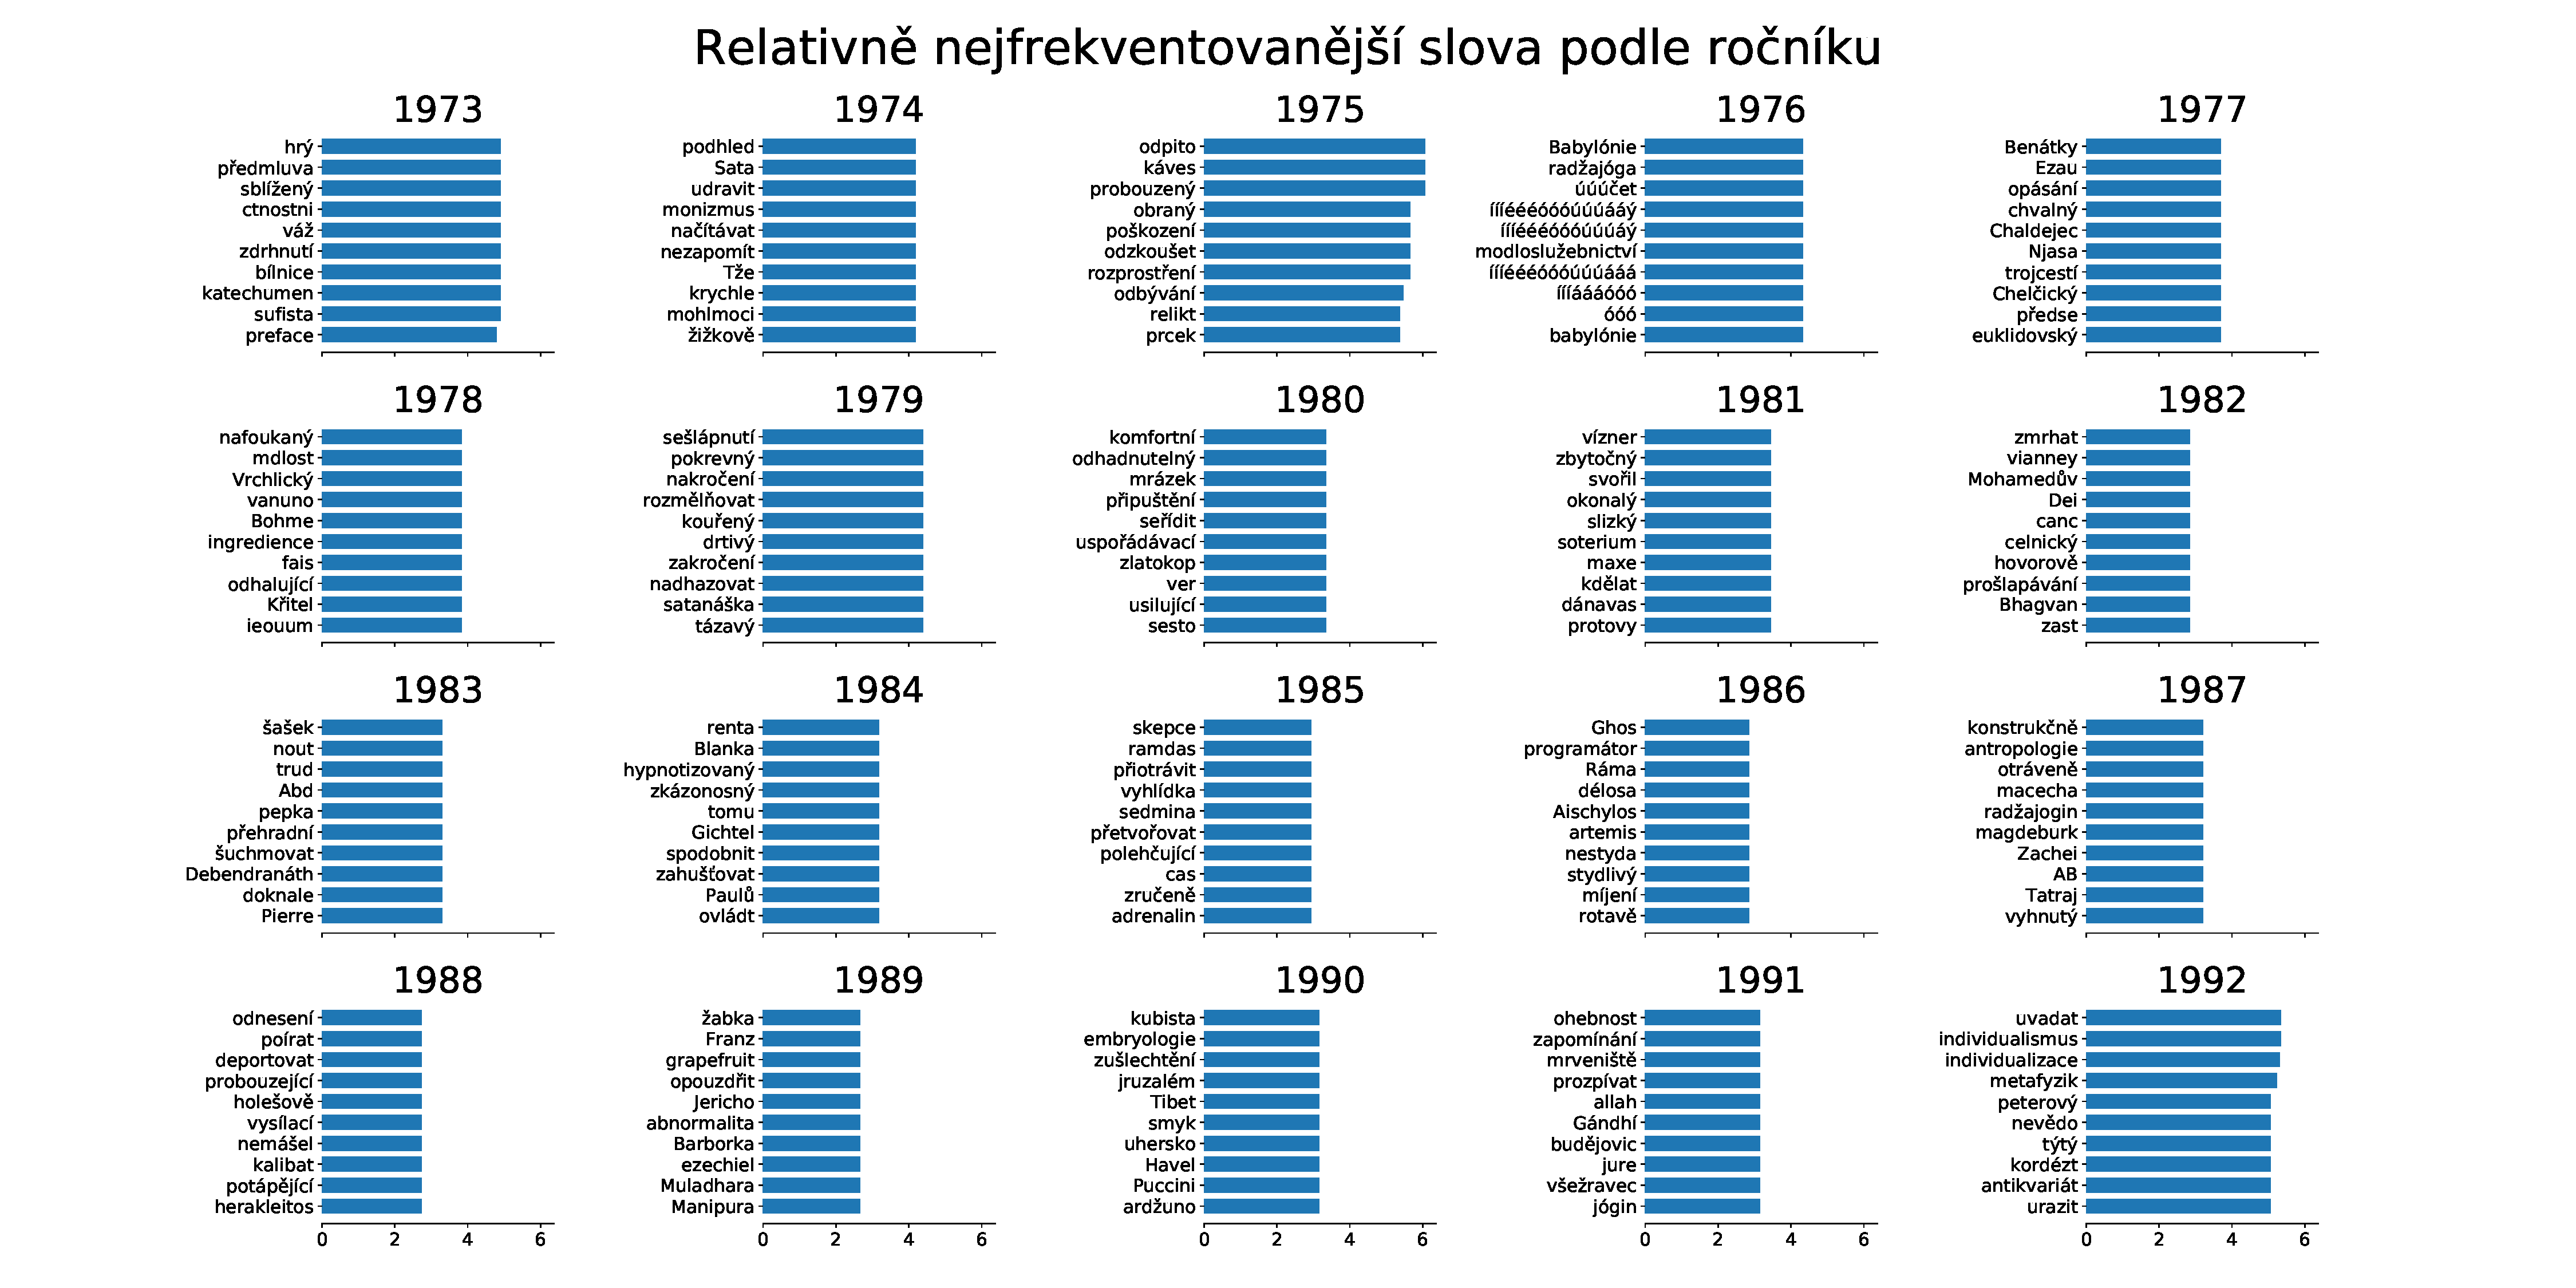
\includegraphics[scale=0.32, angle=90]{rc/topics-by-year-relfreq.pdf}
\caption{Slova s~nejvyšší relativní četností podle ročníku}
\label{fig:topic-by-year-relfreq}
\end{figure}

Naivní řešení je třeba konfrontovat s~řešením založeným za zavedených postupech.
V~oblasti extrakce klíčových slov z~textu je takovým zavedeným postupem
algoritmus \textit{TF-IDF}\cite{Beel2016-11Resea-32348}, anglická zkratka pro
,,term frequency -- inverse document frequency``, čili četnost pojmu -- inverzní
četnost dokumentů. Tento algoritmus upřednostňuje slova, která se vyskytují
často (term frequency) a upozaďuje slova, která se vyskytují často ve všech
dokumentech (inverse document frequency).

Adaptoval a použil jsem systém používající tf-idf jako váhu slov a
Kullbackovu-Leiblerovu divergenci jako míru pro porovnávání dokumentů.
Natrénoval jsem ho opět na celém korpusu Makoňových nahrávek a vyhodnotil pro
ročníky 1973 až 1992, opět po odfiltrování stop-slov a po lemmatizaci. Výsledek
je vidět na obrázku~\ref{fig:topic-by-year-kld}.

\begin{figure}[htpb]
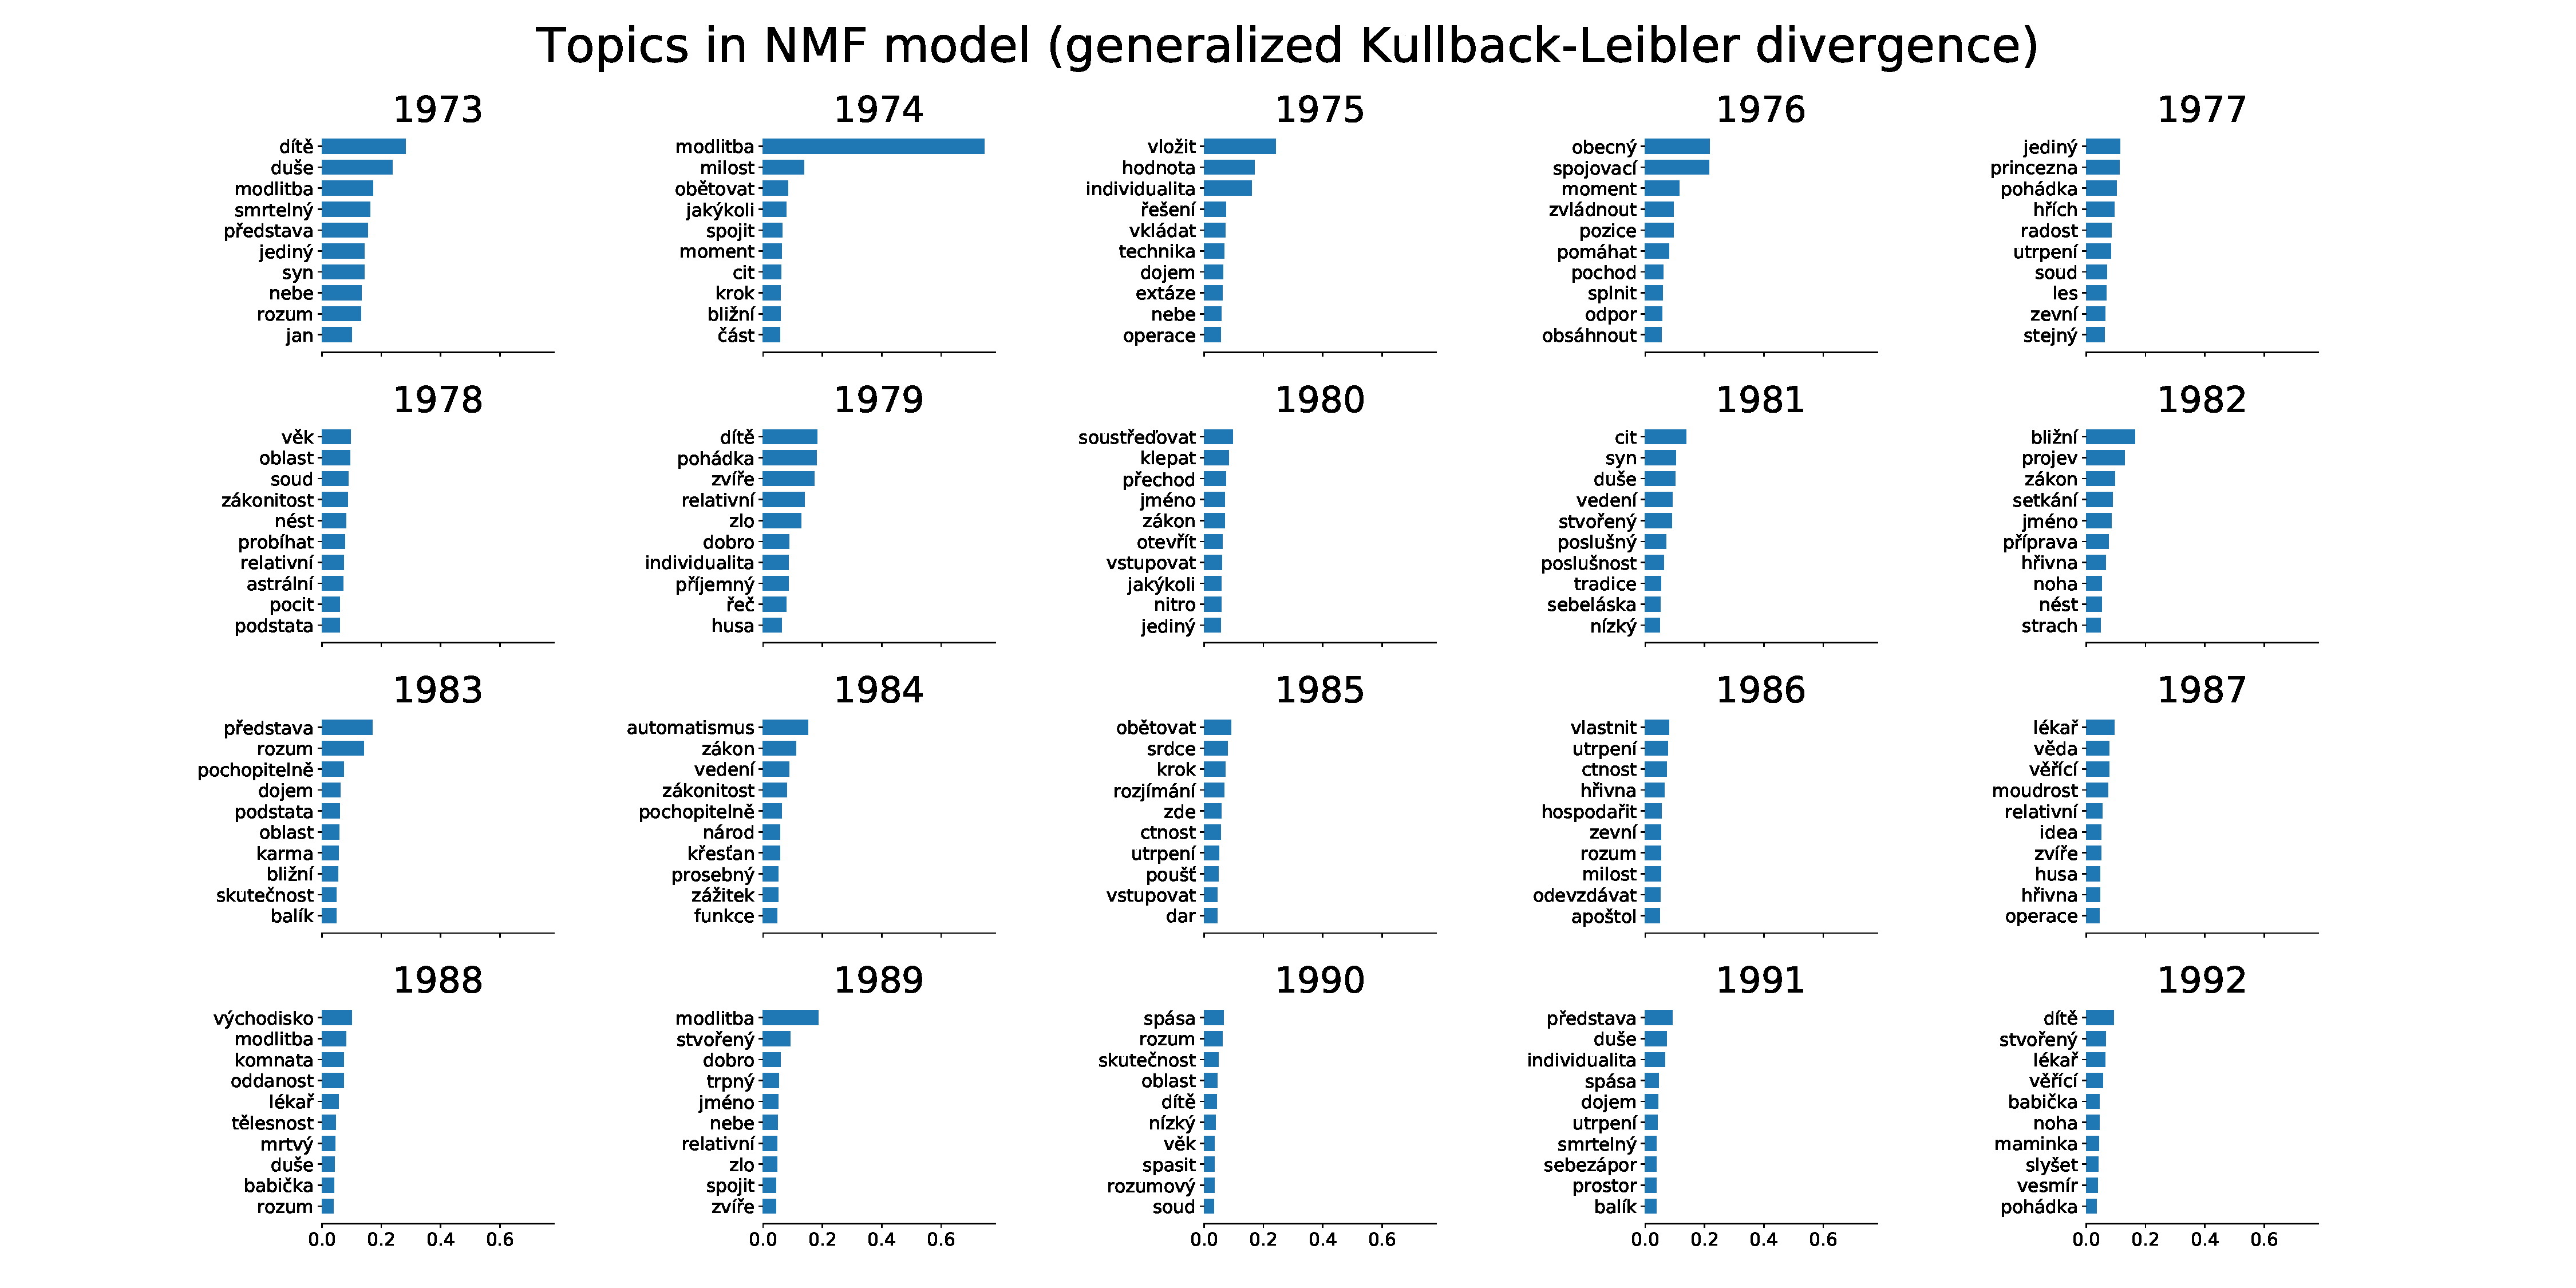
\includegraphics[scale=0.32, angle=90]{rc/topics-by-year-kld.pdf}
\caption{Slova s~nejvyšším skóre TF-IDF oproti Makoňovi podle ročníku}
\label{fig:topic-by-year-kld}
\end{figure}




%utrpení:
%rovnováha mezi vnitřním a vnějším životem;
%nevědomost;
%nutnost odevzdání

%karma

%dobro a zlo

%zákonitost milosti Boží

\chapter{Teologie Karla Makoně}
\label{kap:teologie}

V~kapitole~\ref{kap:temata} jsem se na Makoňovy nahrávky díval jako na zavřenou
krabici neznámého obsahu a pokoušel jsem se do ní z~různých úhlů vrhnout světlo,
aby se ukázalo, co se v~ní nachází. V~této kapitole se chci nadále pokoušet
odpovědět na otázku, co Karel Makoň říká, ovšem z~jiného východiska. Tentokrát
mi nejde o to, pokrýt věrně celý obsah pomyslné krabice, nýbrž si vzít sadu
konkrétních otázek a zjistit, jak na ně Makoň odpovídá.

Za tyto otázky vezmu tradiční body systematicko-teologické nauky:
\begin{enumerate}
    \item{%
        Nauka o Bohu
        \begin{enumerate}
            \item{O Bohu jediném (boží podstata a vlastnosti)}
            \item{Boží trojjedinost}
        \end{enumerate}
    }
    \item{%
        Kosmologie, nauka o stvoření, o Bohu stvořiteli
        \begin{enumerate}
            \item{Bůh stvořitel}
            \item{Boží prozřetelnost: svět je řízen}
        \end{enumerate}
    }
    \item{%
        Antropologie: K~čemu je člověk, jaký má smysl a jak ho porušil
    }
    \item{%
        Christologie
        \begin{enumerate}
            \item{Christologie: o osobě, podstatě, přirozenostech}
            \item{%
                Soteriologie: o Kristově díle; o ospravedlnění v Kristu; o posvěcení
            }
        \end{enumerate}
    }
    \item{%
        Ekleziologie: o církvi, jaká církev je pravá, viditelná / neviditelná církev
        \begin{enumerate}
            \item{%
                Sakramentologie: nauka o svátostech; otázka a Božího slova a svátostí
            }
        \end{enumerate}
    }
    \item{Eschatologie}
\end{enumerate}

\section{O Bohu}

\textit{%
,,Teď bych chtěl říci: Tam hrozilo a hrozí dosud, že když takhle někdo si čte ten
Starý zákon i Nový, tak z Boha udělá bytost. Bůh nikdy bytostí nebyl. Takhle se
nám taky dodneška v~křesťanství Bůh definuje. Je to nejdokonalejší bytost, že
ano, všemohoucí, vševědoucí a tak dále. Kdyby tomu takhle bylo, tak by vůbec
nebylo možno se jinak spojit s~tím Bohem než bytostně. A já, který jsem nechápal
Boha také jinak než bytostně, třebas ne jako starce, to jedno, tak jsem
narazil podle starých Židů a jiných předpisů třebas indických na bytostný
způsob dosahování. Existenční já tomu říkám. Takže moje zkušenosti jsou také
z~tohoto oboru jako bytostné, jsou existenční. Ale jaké v~tom je nebezpečí? Že
totiž ten člověk, který si předělá Boha na bytost, nikdy nepochopí, Bůh tedy je
také stavem. Nebo považuje to za vedlejší, že je stavem. Že je stavem vědomí,
stavem lásky, stavem existence, stavem poznání.``
%My totiž poznáváme takhle lidsky
%tím způsobem, že když to vidíme, cítíme nebo smyslem. Smysly nám to předkládají a
%my to rozumně zpracujeme, tak teprve to považujeme za poznané. To ještě poznané
%vůbec není. Tedy to je jenom porozumění věci, ale my to považujeme za poznané.
%Kdežto kdybychom správně mysleli, jak se myslet má, tak bychom věděli, že abychom
%mohli něco tímto způsobem poznávat, je k~tomu třeba mít
%obecnou schopnost poznávací. Takže když už něco
%konkrétně poznávám, tak to je jenom používání té obecné schopnosti poznávací. A je to
%tedy poměr jako projevu k~neprojevenému. Že my obecný způsob nebo obecnou
%schopnost poznávací nepoznáváme. My víme, že poznáváme, teprve když něco
%konkrétního poznáváme, nebo abstraktního, to už je jedno. Prostě poznáme něco, co
%se nám předkládá k~poznání. ale myslíme si, že kdyby by se nám nic
%nepředkládalo, že by prostě potom nezbylo vůbec nic z~toho, co je v oblasti
%poznání, to je omyl.
}

\textit{%
,,Co se myslí tím, že jdeme k~Bohu jako k ničemu jako k~,,nic``, že ten Duch je
nic? A my, co považujeme za něco, nic vlastně není a tamto nic, co považujeme
za nic, je fakticky všechno? No, něco na tom je. Já tomu nemohu odporovat, této
myšlence, ale já bych rád to ještě z~hlubšího hlediska vysvětlil. Ježíš Kristus
se o tom vyjádřil tak, že on je úhelným kamenem a že ho zavrhli a že potom
nemohou postavit budovu bez toho úhelného kamene, že se to všechno zřítí a že to
nemá základy a podobně. My jsme totiž postaveni svou existencí na tomhletom
,,nic``. To znamená na něčem, co bychom nemohli konkretizovat jako existenci. Pro
nás přeci Bůh neexistuje. To si musíme přiznat. Já aspoň jako beznaboh si to
můžu přiznat. Pro mě do těch sedmnácti let Bůh neexistoval, to jsem byl hotový
beznaboh. A svou silou jsem jím pořád. Jenom mocí Boží chápu to jinak. Ale ze
své schopnosti víry, kterou nemám, bych to nepochopil. Já vás obdivuju. No ale
jestliže tomu takhle je, že ten člověk jde k~něčemu, co neexistuje na žádné
úrovni, nýbrž co ty úrovně jenom řídí, a kdyby to existovalo na úrovni
kterékoliv, tak by to nemohlo řídit. Tak je to to pravé nic, ke kterému se jde.
Po každé úrovni si můžete kráčet, ať je to sebevyšší. Třetí nebe ať je to, tak
po ní můžete kráčet. Se tam procházím mezi... může mi tam být dobře. Ale pravé
Tao není cesta, po které se dá kráčet. To je, to je to pravé nic. Tam až
vstoupíte, do toho nic, tak si uvědomíte s~Lao'c-em, ,,Tao je při všem. Ale do
ničeho nezasahuje. A chceš-li se přiblížiti k tomu Tao, nerozlišuj mezi
příjemným a nepříjemným. Kdo rozlišuje mezi příjemným a nepříjemným, nemůže se
přiblížiti k~pravé moudrosti.`` No, ono se tomu lidově říká: ,,Slunce Boží svítí i na
špinavou kaluž,`` ne? Nerozlišuje. Nesvítí víc do té
čisté kaluže, než do té špinavé, že ano? A v~tom smyslu je to nic. Že je to
vrcholně milosrdné. Ale tak nerozlišeně milosrdné, že už to z~lidského hlediska
jako milosrdenství nemůžeme poznávat. To je tak totálně milující, že z~hlediska
lidského, z~hlediska člověka, který je zvyklý, že láska někam teče, konkrétně
nějakým korytem k~něčemu, k~něčemu se vzpíná, tato láska to není, takže my to
jako lásku poznávat nemůžeme. My i tu lásku Boží poznáváme, jakože neexistuje,
že to nic. A zrovna tak je to s~tím bytím a s~tím poznáním a se vším. Tak bych
to takhle chtěl rozpitvat, abyste viděli, co je to nic. To je všeobsažné.
Na pozadí všeho existující. Ale na \textbf{pozadí} všeho existující. To
znamená, když rozbijete atom na nejmenší ještě další částky a ty zase,
tak Boha nenajdete. Ten není v~něčem existujícím. Ten není
tím existujícím, lépe řečeno. Ale je na pozadí toho. On to všechno udržuje, on
to všechno udržuje při vědomí, při existenci, podle toho, na jaké úrovni se to
vyskytuje, ne? Tak k~tomuto nic jdeme, takže když potom se dostaneme do toho
nic, tak je to pro nás ohromující zkušenost, protože my víme: ,,Je to nic, ale
tím jenom proto, že je to nic, tak je to všecko.`` Já se nedivím, že někdo je
takový pantheista, řekne, tak Bůh je všechno. Je to nesprávný postoj, to já
uznávám, to je velice, velice zvrhlý postoj. On není všecko. Ale všecko je
ustavičně z~něho. Ale má-li být z~něčeho ustavičně něco, jenom z~toho má
pocházet, tak ono to nemůže být tím nebo oním, to nemůže být.% To by se, to by
%potom z toho něčeho potom vycházelo se a Z toho druhého, to druhé už by nemohlo,
%to je, má jinou povahu, z toho vycházet.
To musí být opravdu nic, aby z~toho
všechno mohlo vycházet. Já nevím, to asi nesrozumitelné. Je to srozumitelné? Je
to těžko srozumitelné, no ale je to tak. Protože Pán Bůh kdyby se měl starat o
věci, které řídí, takhle by dopadlo. Nemá ani ruce ani nohy, a tím, že všechno
řídí, tak to vypadá, jako by to neřídil. Jako by byl nic. Tím, že všechno
miluje, tak to vypadá jako by nic nemiloval, protože kdo miluje vraha i toho,
kdo je vražděn, tak prosím vás, co to je? Jaká je to láska? To je nelidská
láska. Jako by ta láska neexistovala. Jakto že tady toho vraha nezastavíš, jakto
že mu nezastavíš ruku, když on vraždí? Co je to za lásku?``
}

\textit{%
,,Já bych to řekl asi nějakým přirovnáním: Bůh je bytost, promiňte, že takhle
budu mluvit, která... nebo jsoucnost, která je schopna nejvyšší možné lásky. Nikdo
není schopen takové lásky jako on, takže my snad můžeme tu hlásku přirovnat
k~lidem, kteří se mají vzájemně rádi. Já to udělám, ovšem samo sebou, že to bude nebe
a dudy ne?``
}

\textit{%
,,Jak líčili ti proroci a ti zasvěcenci toho Boha? Jako krutého mstitele, který
mstí hříchy do třetího a čtvrtého pokolení Já nevím, jak to pokolení k~tomu
vůbec přijde. A krutý mstítel,
soudce a tak dále. Všechno si to můžete v~Starém zákoně přečíst. Ono stačí tahleta
charakteristika. Co to je za vtip, takhle líčit milosrdného Boha? To je úžasně
moudré.
Protože jestliže člověk nevidí, neví o tom, že když je v~této fázi, že je na úrovni
přírodní, kde platí oko za oko, zub za zub, kde silnější má právo a neprohřešuje
se tím,  zabíjet toho slabšího nebo toho nemocného, tak nevychází z~údivu a
myslí si,
že je Bohem opuštěn. Ne, ten bůh se jeví tomu králíku jako absolutně
neexistující,
nebo když existující, tak jako nemilosrdný soudce, protože když ho přepadne orel,
tak je odsouzen k~zániku a žádný pán Bůh mu nepomůže, ani prstem nehne. A na to
vás upozorňuju, že kdykoli upadneme do stavu přírodního člověka, to znamená na
tom světě jenom jíme, pijeme, spíme a máme se dobře jako zvíře, tak není pro nás
žadné milosrdenství Boží připraveno, je pro nás připravenn Bůh nemilosrdný,
soudce, který bude trestat naše hříchy do třetího a čtvrtého pokolení.``
}

\section{Trinitologie}

\textit{%
,,Bohu nelze rozumět. A to je to, čím bych chtěl začít. Proč mu nelze rozumět?
Proč se s~ním
nelze setkat? Proč ho nelze vidět? To bych chtěl dopovědět proto, že existuje
Bůh,
který je vlastně trojjediný. To vědí Indové, to vědí Evropané, to vědí křesťani,
tedy všichni na světě. Staří národové. To věděli Sumerové. Co to je ta
trojjedinost? My si řekneme otec, duch a syn a tím to
vyřídíme. Nic jsme tím nevysvětlili. Naopak jsme zatemnili věc. Jsou to, řek bych
školsky, rozdělené funkce jednoho a téhož Boha. Funkce, čili úkoly, které na sebe
vzal nebo ustavičně bere jeden a tentýž Bůh Ten totiž má úkol stvořitelský,
kterýž ustavičně tvoří, a tentýž Bůh má úkol spasitelský, že to stvořené k~sobě
táhne. Teď si už jenom představte, jak je těžké porozumět jednání takového Boha,
který zároveň ustavičně něco od sebe z~domova posílá do světa od sebe pryč a zároveň
z~toho světa to táhne k~sobě. Jak rozeznat jednoho od druhého? Jak to oddělit?
Z~toho byli věřící
v~koncentráku úplně vedle. Všichni věřící, se kterými jsem se tam setkal.
Všichno říkali: ,jak se
na tohleto zvěrstvo může dívat pán Bůh? Jak mě může nechat takhle na holičkách?
Já
jsem přeci byl vždycky zbožný člověk a já tady takhle trpím bez pomoci a takový
zvíře gestapácký má na mě všechna práva a Bůh ani prstem nehne pro mě.`` A kdykoliv
jsem s~nimi souhlasil a takhle myslel, vždycky [jsem] dostal nějaký kopanec od
toho gestapáka. Zrovna! Přesně! To je řízení od pána Boha, opravdu, abych věděl, že
pán Bůh s~tím absolutně souhlasí, že takhle se o člověka nestará. Ale vedle
tohoto,
vedle těchto dvou principů Božích -- stvořitele a spasitele, existuje třetí jeho princip a
to jest, oni říkají křesťani ,potěšitele`, ale lépe bylo řečeno osvětitele, že
opravdu ten člověk vlivem toho Božího působení v~něm může být čím dál
osvícenější. Že nemusí slepě jít ani od toho Boha pryč, ani k~tomu Bohu
nazpátek,
nýbrž může plně s~plným vědomím vědět, co dělá. Velice nutné, aby tento třetí
princip tam taky existoval u toho Boha.``
}

% 82-22 55:16
\textit{%
,,Otec, Syn a Duch svatý. My si totiž nedovedeme vůbec představit, jak je
to možný, že na jedné straně pán Bůh něco tvoří a ustavičně to tvoří -- kdyby to
ustavičně netvořil, tak my nejsme vůbec na světě, jo? Musí pořád do toho svoji
bytostnou, podstatnou část vkládat, aby mohl existovat tady kámen, čas a prostor
jako celek a taky tedy člověk, čili to je proud, který míří od něho do
časoprostoru. Kdybyste se, jako normální člověk je, spojili jenom s~tímto
proudem,
to znamená žili si jenom pro sebe, tedy z~toho, co od něho dostáváte, aniž si
uvědomíte, že z~toho žijete, tak promrháte všecko. Ne protože byste se nechytli
toho druhého proudu, kterým je spasitel a to je tentýž Bůh, ne nějaký druhý,
jenomže zároveň s~touto silou odstředivou působí síla dostředivá. Vzájemně se drží
v~šachu, ano? Protože když máte odstředivou sílu deset a dostředivou deset,
deset bez desíti je nula a to je Bůh. A jsou tam obě dvě tyto síly, rozumíte mi
dobře? I ta desítka kladná i ta desítka záporná a přesto je to nula, že jo? To je
to nic přirozenosti Boží. Nesmírně veliká moc tvůrčí, nesmírně veliká moc
spasitelská. A co je to, to třetí? Ten Bůh utěšitel nebo osvětitel, Duch svatý?
To je zase něco, a o to se hádali katolíci s~pravoslavnými, jestli Duch svatý působí
jenom přes Ježíše nebo taky... jestli taky přes Ježíše a nejenom z Otce.
Pravoslavní říkají, že jenom z~Otce pochází, a katolíci, že pochází také ze
Syna,
vychází taky ze Syna. A roku tisíc našeho letopočtu se rozešli a vznikla
Pravoslavná církev z toho, to byly ještě důvody nějaký politický, ale to nevadí.
Zkrátka pro takovou maličkost se rozešli a byl to zbytečný
rozchod. Dneska by se to už mělo uspořádat, protože ona je to síla, která
působí skrze obojí. Je to jenom další funkce Boží, která se nedá vysvětlit plus
deset a mínus deset, nýbrž by se musela vysvětlit úplně jiným obrazem. Já ho
tady nebudu předvádět, protože to by byl obraz na čtvrt hodiny, ale je to síla
poznání,
se kterou si vůbec křesťané zatím nevěděli rady, a to z~toho důvodu, že je třeba
napřed tu kladnou desítku s~tou zápornou desítkou vyrovnat a teprve potom může
nastoupit ten Duch svatý.``
}

% 79-01 01:06:10
\textit{%
,,Tady nemějte starost, že by na tomto předělu vám nekynula žádná pomoc. Ta pomoc
je vyššího druhu a není závislá už od vedení událostmi nebo od vedení stvořením,
stvořeným nebo naším já, nýbrž je závislá jenom čistě na tom Bohu, který je jiným
Bohem než který tvoří a o kterém se vyjádřil Eckhart, že nemá nic společného
s~Bohem, který je stvořitelem, ano? Je to tentýž Bůh, ale je to jiná jeho tvář, která
nemá nic společného s~tím Bohem, který je stvořitelem.``
}

% 76-03A-Kaly-5 23:22
\textit{%
,,My totiž pořád slavíme trojici Boží: Bůh Otec, Bůh Syn a Bůh Duch svatý, ne?
Ale to synovství Otcovo nemůže být ve stavu určité míry oddělenosti, jak se to
jevilo po ty tři roky, kdy on poslouchal, ale byl menší než Otec. Potom až se
znovu stane synem, až se mu vrátí synovství na jiné úrovni, tak už bude roven
tomu Otci. On bude mít právo poslat Ducha svatého. A takhle bude vládnout celým
Božstvím, celým obsahem jeho moci. A ta moc největší spočívá v~tom vedení Duchem
svatým všeho. Ten Duch svatý ve všem vládne, ve všem je pravou živou podstatou.
Ten Duch svatý totiž je podstatou všech těch samovolných sil. Ten se ocitá na
jejich podkladě. Ale zatímco ty síly samy o sobě jsou trpné, On je přitom
aktivní, víte? To je ta stránka aktivní těch samovolných sil.``
}

\section{Stvoření}

% 82-02 42:07
\textit{%
,,Můžeme se opřít o vědecké bádání: archeologické bádání, antropologické bádání,
o všechny možný druhy věd se můžeme opřít a víme tohleto: Že na tom světě se
vyvíjeli napřed jednodušší tvorové, ale vždycky současně zvířecí říše
s~rostlinnou. Tato symbióza mezi zvířetem a rostlinou existuje od začátku toho
života na tomto světě, víte? Takže nedegradujme rostlinu na úroveň pod zvíře. To
je směr jdoucí jinam, než kam jde zvířecí život. Tyto dva musí být vedle sebe se
specializovaným úkolem, aby to vůbec všechno mohlo fungovat. Bez zvířat by
nebyla rostlina a bez rostliny by nebylo zvíře, tak to asi zjednodušeně je. Já
to dělám všechno velice zjednodušeně, školsky. A bez těch dvou by nebyl zase
člověk, To je taková nadstavba nad tímhletím. Ovšem člověk je na straně těch
zvířat, nikoli na straně rostlin. A tak teďka především bych byl rád, kdybyste
věděli, že do této vývojové teorie nemá vůbec co mluvit povídání Geneze ze
Starého zákona, že za šest dní Bůh něco stvořil a sedmý den odpočíval. Vůbec o
tom se tam nemluví. I když je tam jasně řečeno: ,,Napřed bylo to, potom bylo
tamto.`` To vůbec nemá souvislost s~dnešním pochopením vědy a nic to nemluví
proti dnešnímu pochopení vědy. Rádo se to staví jedno proti druhému, ale je tam
je to líčení stavu a tady je to líčení situace, že?. Dnešní věda si zkoumá
situaci, vývoj situační. Kdežto tam se mluví o stavové situacei, stavovém stavu.
Já bych tamto řekl takhle: Jestliže by v~člověku neexistovalo na té úrovni, na
které on je, šest dní tvůrčích Božích a sedmý den odpočinku Božího, tak on jako
člověk by nemohl ani prstem hnout směrem ze své úrovně. On by nemohl zdvihnout
hlavu k~Bohu.``
}

% kotouc-D01-d 01:00:15
%\textit{%
%,,My si představujeme, že Ježíš Kristus to jednou odnes na tom kříži a že nás
%tím spasil, a takhle to je klamný dojem. To jsou všechno symboly toho,
%co se věčně děje. Zrovnatak dejme tomu stvoření světa je
%symbol toho, co se věčně děje, ustavičně probíhá v~tom vesmíru. První den stvoření
%světa, druhý, třetí, čtvrtý, pátý, šestý i to odpočívání. Všechno tam souběžně
%probíhá.
%Ono se to nedá znázornit nijak jinak než jako děj, ale ono to vlastně je
%permanentní situace, ustavičně se opakující. Takže ten Ježíš je ustavičně
%například křižován, ale také ustavičně vstává z~mrtvých. Teď je otázka, jestil my
%se s~ním dáme ukřižovat jenom a jestli my s~ním vstaneme z~mrtvých a nebo
%ne.``
%}

% kotouc-T01-metoda-d 01:24:55
\textit{%
,,Ježíš v~té době svého mládí trošičku viděl víc do té činnosti svého Otce než
my. Bylo to způsobeno tím, že prošel narozením v~Betlémě, což nebylo obyčejné
narození. To je symbol už velice vznešeného znovuzrození, velice vznešeného
znovuzrození a my jsme tím neprošli, tak proto takhle nevidíme do dílny Boží. A
kdybych tedy, pokud si to dovedu vůbec představit, měl říci, jakým způsobem asi
Ježíš Kristus viděl do ty dílny Boží a proto viděl, že musí být v~tom, co je jeho
Otce, tak bych to řekl asi takhle: On už dobře znal, že to, co je ve Starém zákoně
pověděno o šesti dnech práce Hospodina a sedmém dnu odpočinku, že to je symbol
toho, co se ustavičně děje. Co ustavičně probíhá. Že probíhá ustavičně činnost Boží
a ustavičně sedmý den odpočinku. Kdo tohleto zažil, tak ví, že stvoření potom má
zcela jinou povahu, než jak my podle symboliky, kterou si nedovedeme zatím
vysvětlit, mu
přičítáme. Že totiž to není nějaká akce, po ní zase následuje další akce, ta tvůrčí
činnost Boží, jako je to tam líčeno, nýbrž že je to soustavná činnost na různých
úrovních, jak je to tam líčeno, neboť nedokážeme to jinak vyjádřit než symbolem
času a prostoru a pak to musím líčit jedno za druhým, když to jednou dáme do času
a do prostoru. Ale když to obrátíme, když z~toho symbolu přejdeme do té
bezčasovosti,
ve které se to děje, ze které to prýští, tak tam se zároveň rodí svět a zároveň se
ničí, zároveň je Bůh v~klidu. A kdyby tomu tak nebylo, tak my nikdy nemůžeme být
činní, protože on je jediný činitel. Jak bychom my mohli být činni, kdyby on
činitelem nebyl? Naše činnost je odvozena od činnosti Boží. Uboze odvozena od
činnosti Boží.
On je jediný činitel. Ale bychom nikdy nemohli být v~klidu, kdyby on v~klidu
nebyl.
Nikdy ne. A protože on je neustále v~klidu, a náš klid je odvozen z~jeho klidu,
tak také můžeme v~klidu být.``
}

\section{Řízení světa}

% 83-05 17:00
\textit{%
,,Vidíme, že je tady nějaká hierarchie. Nějaký řádově vyšší a nižší způsob
života. Jenomže není nám dáno, abychom hleděli za hranice tohoto časoprostoru,
abychom věděli, jestli tento řád pokračuje dál. Jenže byli lidé a jsou lidé,
kteří rozšířili svoje vědomí a vědí, že to co se nám tady jeví jako nějaký řád
hodnot, jako nějaká podřízenost nadřízenost a tak dále i v myšlenkovém světě,
jako například je znázorněno v Otčenáši, tam je znázorněna ta podřízenost tím
seřazením těch modliteb, tak jestliže jsou tady lidé, kteří o tom to vědí a
jestliže jim můžeme věřit nebo se můžeme dokonce přesvědčit, že mají pravdu, tak
pak bychom neměli pochyb o tom, že Bůh má smysl. Že v~tomto řádu musí být nějaký
vrchol a musí být nějaký spodek. Jestliže toto všechno tady na světě je, při
pouhém pohledu na tento svět, tak můžeme klidně předpokládat, že toto platí za
hranicemi této zákonitosti. Že existujou jiné ohrady, širší, zákonitost vyšší,
svobodnější a za jiných okolností probíhající a tak to jde dál, až možná tam na
vršku je něco nad tím zákonem. A to je v pořádku, protože já když lidsky na tom
jenom tak jdu, tak si řeknu: ,Je-li tady nějaký zákon, tak to přeci předpokládá
nějakého zákonodárce. Takže smysl Boha, to je smysl zákonodárce.` Ovšem dívat se
na Boha jenom jako na zákonodárce, to je chabý pohled. Já se zatím na to omezím,
protože nechci... o Bohu by se dala přednáška udělat, přednáším o Bohu asi
padesát dva let a nemá to konce, takže já se omezím na tenhleten postoj a řeknu,
že tedy smysl Boží je, že něco musí být řízeno tak, musí být řízeno tak, aniž
víme proč, musí být řízeno tak, aby to nebylo vidět, že je to řízeno. Protože
kdyby všechno bylo řízeno tak, aby bylo vidět, že je to řízeno, tak by se to
nedalo vůbec řídit. To je ten hlavní důvod. Já ty ostatní důvody, těch je
stovky, nebudu jmenovat, ale víte, že mnoho věcí probíhá ve vaší duši, které
vědomě neřídíte, ve vašem těle zrovna tak. Já budu mluvit jako k lékařům. To je
automatismus ve vás živý: srdce, pohyb srdce, že ano, a nevíte, nestaráte se o
to, ne? Jenom že to přiživujete nějak a solidním způsobem žijete, tak to ono
funguje. Má to smysl o tom vědět? Nemá. A proto je nesmyslné vědět něco o Bohu,
který takhle samovolně řídí. Ten nepřemýšlí o tom řízení, vůbec ne. Samovolně
řídí shora, a to je naše pravlast, se všechno řídí tou mocí této samovolnosti.
To je obrovská moc. To je tak velká moc, viď, vy jako lékaři to nejlíp pochopíte
ze všech lidí. jaká je to obrovská moc toho automatismu, já mu říkám
[automatismus] jedna, který v~nás řídí všechen průběh vnitřních sekrecí a
klepání srdce a pohybu střev a to všechno dohromady a harmonizuje to dohromady,
ne? A my jsme k~tomu přišli jako slepí k houslím, ne?. Jak je to dobře, že my
jsme tomu takhle přišli. Ne že bychom o tom neměli nic vědět, ale že to tady je.
Atak je taky dobře, že je tady tenhleten Bůh, že to takhle samovolně všechno jde
až nahoru, tam my vůbec nedozírnem. Ale ono se to dá rozšířit a smysl právě toho
lidského života, který jde za hranice toho toho normálního vidění, spočívá v
tom, že člověk rozšiřuje svoje vědomí do těch oblastí, kde už vlivem své morální
vyspělosti je schopen zasáhnout jako pán Bůh. Řek bych bez protivenství vůči
Bohu, bez zásahu do vůle Boží. To znamená se zřeknutím se vlastní vůle a se
ctění nějaké vůle vyšší. Takže smysl toho celého je umět se podřídit vůli, která
je moudřejší.``
}

\textit{%
,,To si myslíte, že není vůbec možné. Že se od té doby zázraky nedějí, ale
je to z~toho důvodu, že mu nedovolujete, aby vstoupil do vašeho života.
Například tady že vstoupil tady doktor Elger zrovna v~okamžiku, než jsem to tam
chtěl začít vykládat, on považuje za režii. Já zase vím, že je to právo, které jsem
dal Ježíši, aby vstoupil do jeho života. Žádná režie. Já mám právo také dávat,
pokud se mi lidé dají, on se včera dal, právo, aby vstoupil on do jejich života,
víte? Protože nesmíte se cítit oddělenou bytostí, ne? A když mně ukáže, jako se
to stalo v~koncentráku poprvně: ,Těch pět mně přivedeš,` ne? tak to právo trvá,
ne? Žádná režie. To je právo. A ty máš taky právo -- každý má právo -- do života Ježíše
pozvat. To nebyla režie, to byla součást toho, že já jsem pozval do tvého
života Ježíše, rozumíš? Mně nejde o slovíčka. Mně by nemuselo vadit, že to
považujete za režii, ale já nechci ubírat tomu pánu Bohu na jeho cti. Nechci
ubírat na tom pochopení jeho úmyslu. On nechce váš zivot režírovat, nýbrž on
chce,
abyste mu patřili. On tebe teďka pozval k~tomu, aby ses naučil mu lépe patřit,
rozumíš? Jestli v~tom vidíš režii, já v~tom vidím pozvání.``
}

\section{Antropologie}

% 85-05A 05:14
\textit{%
,,Aby včelí rod byl zachován, ona nemůže mít lidský rozum, ona nemůže mít mozek.
To je veliká vymoženost, že nemá mozek. Centrálně by nedokázala to, co dokáže
včela decentrálním rozmístěním čidel, které nahrazují mozek, provést. Takže
včela může bezvadným, naprosto neomylným způsobem letět za květem, který je
vzdálen, který necítí a za kterým ona letí s naprostou bezpečností a přistane na
tom květu, který jí ukázala ta včela, která je tam... která ji tam navedla,
ráno. A to je spo- způsob, kterým- do kterýho nikdy nedorosteme. Protože místo
toho máme mozek. A ten nám toto neskýtá. A protože nám skýtá něco jiného. Nám
skýtá touhu přerůst přes svůj druh. Já chci být lepší, dokonalejší, rozumnější,
moudřejší, než byli moji rodiče. A proto mládež první chybu, kterou dělá, že se
staví na zadní nohy a říká: "Moje... moji předkové byli hloupí proti mně." To je
první š- špatný pohled, chybný pohled na rodiče a na předcházející generaci.
Voni mají za sebou tohle, to je ten pochod kupředu už totiž. A proto se jim
tamto s- zdá být zaostalé. To, co oni právě zažívají, není to pravda. Voni si
prošli tou fází, kterou ta mládež teprve prochází, aby dospěli do nějaké úrovně,
za kterou už se beztak nemůže jít. A to voni neví, že voni taky dospějou do té
fáze, za kterou už nebudou moct jít. Neboť člověk má taky omezené možnosti. No a
tohleto prostě u těch nižších tvorů také existuje. Jenže ta první fáze toho
mládí, až na slony a některé vyspělé ty savce, probíhá velice rychle. Například
mládí u takové třebas mouchy, probíhá v půl dny, co... co my musíme dělat
osmnáct let, tak ona za půl dne je s tím hotova a je hotovou mouchou lítající a
umí lítat z toho automatismu, který v ní je. Čili my ten automatismus opravdu,
co- který v sobě máme také a máme ho daleko složitější, máme ho dok-
dokonalejší, nemáš- než má třebas husa nebo včela. Ale my ho držíme v šachu. My
mu nedovolujeme, aby se rozrůstal tam, kam se rozrůstá třebas v oblasti prácem-
včely. To znamená, toto nechci přírodovědecky tady dál rozvádět, to by vás
strašně unavovalo. Ale já zůstanu u člověka. A řšš- teď to už chápete, že já
jsem se musel vzdát třebas přírodovědy ve svých patnácti letech. Jak je to
dobře, že jsem se toho musel vzdát, protože já bych z této strany do tý
přírodovědy byl nikdy nevnikl. Dneska do tý přírodovědy vnikám způsobem, kterým
málokterý přírodovědec do toho vniká. A závidí mně, když se s ním setkám, žes...
mám tento přístup k věcem. No, ale nechci se tím chlubit, to jsem já nezavinil,
to zavinili lékaři. Tak, teď chci říci: Jestliže člověk je jediný z tvorů, který
touží po tom, aby přerostl svého druha, aby byl lepší. Nebo dokonce horší, což
je taky svým způsobem jiný. Aby byl jiný, než byl ten vedlejší tvor. To je neb-
aby nebyl stádový. Tak je to známka toho, že dorůstá do pravé individuality,
která od všech relativností je oproštěna. To je ta věčná individualita, ze které
všechno jsme vzali a do které se zase nazpátek vracíme. Od Boha přicházíme a k
Bohu se vracíme.``
}

% 80-07A 36:16
\textit{%
,,Tam budete konvergovat k~Bohu. A teprve tady se občas snažíte, abyste se mu
přiblížili. Ale tam se mu budete věčně přibližovat. To je úděl bohužel člověka.
Budete věčně poznamenání jeho svořitel úkolem. A dobře nám tak. Jinak bychom
nemohli v~tom jeho stvořitelském úkolu fungovat na věky. A ono se od nás chce,
abychom navěky v~něm fungovali. On nás nepotřebuje jenom, abychom byli
spasitelé, on nás potřebuje, abychom byli spolustvořitelé. Spolustvořitelé.
Abychom v~jeho stvoření pokračovali. Jako jsme plodili tady děti, tím jsme se
stávali spolustvořitelé, tak potom chce, abychom zplodili duchovní bytosti.
Budeme dělat totéž. Budeme plodit, pořád budeme plodit, ale na jiné úrovni. Toto
plození na jiné úrovni, ale soustavné, už bez mezer, bude naše nebe.``
}

% kotouc-F01-b    13:00
\textit{%
,,Kámen je udržován v~existenci tím, že ustavičně svou existenci do něho Bůh
předává, ale to je kámen. U rostlin je to zase už lepší, tam se toho předává
víc, aby
mohla růst dokonce, a u člověka se předává největší míra těch vlastností Božích.
Tam se předává značná míra existenční, [proto] má velice složitý organismus proti
kameni, souhra buněk a to všecko a organický život je vůbec složitější než
anorganický, ale předává
se do něho také značná míra uvědomovací síly. On si uvědomuje tento svět do
takové míry, že z~něho si může analogicky vydedukovat život věčný. Může mít pojetí
o životu věčným. Dokud toto pojetí nemá, dokud se nedovede vmyslit, že
existuje věčný život, tak nemůže do něho vejít. A to zvíře si nedovede udělat
ještě. A člověk si může. Nemůžete zatoužit po něčem, o čem nic nevíte, co si
nedovedete
nějak představit, že to existuje, že ano? A člověk tuto představu může pojmout a
právě toto může za touto představou jít. On si vytvoří napřed představu a v~tom je
ztělesněno tolik síly od Boha, že pomocí představy která třeba ještě neodpovídá
zdaleka skutečnosti, jaká existuje za tou představou, se odebere do té skutečnosti
vyšší. Tak proto je život lidský připraven pro tyto vlastnosti, které má, katomu
přechodu do věčnosti. A žádný jiný život není připraven.``
}

\textit{%
,,Ten Ježíš tady není, neexistuje pro mou radost, nýbrž proto že beze mě by
nevyrostl do Jordánu. Lidský život má takovou nesmírnou cenu, že bez něho by se ve
vesmíru Bůh nevyvinul ve spasitele. To je závažný slovo. My máme tvůrčí úkol nebo ještě víc
než tvůrčí úkol, prostě transformační úkol. My jsme transformační stanice něčeho
časného na věčné a bez této transformační stanice ani Bůh nedokáže z~vesmíru
udělat zase sám sebe. Jedině pomocí těchto transformátorů to dokáže a proto nám
posílá spasitele a proto od nás chce abychom ho následovali a tak dále.``
}

\section{Christologie}

% 83-23A-K 39:42
%\textit{%
%,,Vy jste v~manželství s~tímto světem, o tom ani chvíli mě nenecháváme na
%pochybách. vás že tomu taky ale jiné manželství ten navázali když jste mu dokonale věrni a proto jakékoliv rady to je házení hrachu na stěnu. ježíš kristus navázal manželství jiné než mi to Já myslím, že když se narodil na tento svět, že mu nebylo jasno kým je. ale měl předpoklady pro to já vám řeknu které ne tím že byl avatarem aby brzo navázal nové řekl bych spojení nového uvozovkách spojení protože to manželství s bohem naše starší než ten náš původ od Otce je starší než jakýkoliv původ od čehokoliv jiného.``
%}

% 84-27B-p 20:00
\textit{%
,,Ježíšovo učení jestliže se chápe jenom podle toho, co řekl, tak se nikdy
pochopit správně nemůže. Ono se taky nepochopí ani s~tím, co se dělo.
Ale to, co se dělo vedle toho, co říkal je stejně důležité nebo ještě důležitější
možná než to, co říká. Já myslím, že to co říkal je komentář k~tomu, co udělal,
ano? A
tak si všimněme, co udělal do třicátýho roku, co udělal od třicátého roku do
třiatřicátého, a co udělal potom. Vysvětleme si to jenom těmito třemi
periodami. Do toho svého třicátého roku nebyl učitelem, ne? Oslňoval svou
moudrostí,
ale nebyl učitelem. Byl poddán své rodině. Kdyby byl ustrnul na této úrovni, kdyby byl
nešel do Jordánu, nedal se pokřtít, nedal se svádět Satanem -- svým já -- nevzepřel
se mu, protože on potřeboval nám ukázat, že musíme se odpoutat od svého já takovým
způsobem, že nám nemá co do toho našeho chtění co mluvit, jo? Ne, co si přeje
ten Satan, to je to liské já, které si něco přeje vzhledem k~situaci, ve které byl
Ježíš Kristus, měl obrovskou moc k~dispozici, si to jáčko mohlo zase více přát
než u nás obyčejných lidí si přeje. A ono si přálo, aby proměnil chleby nebo kameny
v~chleby, aby seskočil z~nějaké věže a tak dále, aby se mu klaněl a podobně. A on
říkal... jo a ten Satan mu taky říká: ,ale ono je to psáno ve svatém písmu. Když ty
jako to neuděláš, tak ti nikdo neuvěří, že jsi opravdovým spasitelem.` A on to přesto
neudělal z~toho principu, že jedině Bohu je se klanět. Takže teď bych k~tomu chtěl
dodat: Jestliže třebas Ježíš Kristus učí svoje učedníky, prochází světem tehdejším
a dělá nějaké zázraky, tak to je fáze, o které se vyjádřil, že je menší než
Otec, za
prvé a jenom o té fázi se tak vyjádřil, za druhé, že nemůže jim zvěstovat to,
co by ještě nepochopili, protože to jim může dát jenom Duch svatý -- pochopení. Čili
je v~tom vidět takový proces vzestupu ve veškerém jeho konání. Co udělal pro své
učedníky po zmrtvýchvstání, po seslání Ducha svatého, nemohl pro ně udělat v~tom
období učitelství, kdy byli jenom jeho učedníky, ano?``
}

% 77-05B-Praha 16:40
\textit{%
,,Takže tím jsem řekl, že Ježíš je projev Boha. Projev Boha živého a že to
není Bůh. Projev Boha živého, ovšem daleko vznešenější, než jsme my, ale menší
než Otec. A proto jestliže má přejít na pravici jeho, znamená má mu být
roven, jako on o sobě říká, že se to stane, tak on se musí vzdát toho synovství.
Ne že by o to nestál, ale že je to
málo. Že je to jenom prostředek, Ježíš je prostředkem k~tomu, abych se dostal
k~Otci, ne? On nikdy
nikomu neříkal, že vede k~sobě, nýbrž vede do Království Božího, k~Otci, do domu Otcova a
tak dále. Že on je prostředkem, ničím více než prostředkem. No, čili Kristus je
od věky Bohem.
Ježíš je dočasně daným prostředkem vývojově dokázaným, to znamená: Je tam
ukázáno,
jakými proměnami ten prostředek, který nám dává k~dispozici, musí projít, aby se
člověk pomocí téhož prostředku dostal až na to nebe, byl tam  vzat, jak se říká, a ono je
to tak, že opravdu ten prostředek, který ze začátku vypadá jako malý dítě,
nemluvně, se
nám později jeví jako někdo úplně jiný. Za chvilinku je tesařem a za chvilinku je
učitelem a opět za ještě menší chvíli umírá na kříži.``
}

% 83-23A-K 39:42 -- manželství se světem
\textit{%
,,Ježíš Kristus navázal manželství jiné než my. Já myslím, že když se narodil na
tento svět, že mu nebylo jasno kým je. Měl předpoklady pro to, já vám řeknu
které -- ne tím, že byl avatarem -- aby brzo navázal nové, řekl bych spojení
nového v~uvozovkách spojení, protože to manželství s~Bohem naše je starší než...
ten náš původ od Otce je starší než jakýkoliv původ od čehokoliv jiného, co
mezitím bylo původem, také ale už odvozeným.``
}

\section{Soteriologie}

\textit{%
,,Jestliže Ježíš Kristus řekl: ,Já jsem cesta, pravda a život,` řekl, jakou
funkci Boží on zastává jako spasitel.``
}

\textit{%
,,Současně probíhá odtvořování. To znamená, že Bůh také všechno miluje. Všechno
stvořené miluje a k~sobě táhne. A věci dospěly tak daleko, že bylo třeba jim to
názorně ukázat. Že [je] to názorná ukázka toho spasitelského úkolu Božího, který
od začátku stvoření tu jest. Čili neberte to utrpení Ježíše Krista za věc, která
se jenom stala, nýbrž za něco, co ustavičně jest, a to je rozdíl. Když my jsme
byli svědky jenom toho, přímo nebo nepřímo, co se stalo, to je málo. Teprve když
člověk vnikne do nesmrtelné podstaty Boží, poznává, co jest, a ví tedy, že také
jest ta láska Boží, která tvoří a odtvořuje a samozřejmě osvěcuje. [...] A potom
samosebou se celé to utrpení Ježíše Krista dostává do nového světla. Ne že by
byl on nepotřeboval, proto že jenom to ukazoval, trpět méně. Kdepak? On
soustředěně na sebe bral v~té chvíli utrpení všeho stvořeného a soustředěněji
trpěl, než jak trpí člověk, který trpí jenom za sebe. On za sebe vůbec netrpěl.
On to nedělal, ani toto nedělal pro sebe! I tady platí jeho slova: ,Kdybych něco
dělal pro sebe, nevěřte mně.` On ani toto utrpení nedělal pro sebe. Všechno pro
nás. Bylo třeba... prostě věci dospěly tak daleko, že musel nám to ukázat. Ale
nic nového se nestalo. To všechno jest a trvá. To tehdy ukázal. Čili ještě
jednou jinými slovy: To, co Ježíš ukazuje, to je lidové podání pro lidi určené,
lidové podání zákona, věčného zákona, který funguje ve veškerém stvořeném. A ten
zákon zní: Kdyby Bůh nemiloval stvořené, vůbec by ho byl nestvořil. Protože ho
miluje, tak ho zároveň k~sobě táhne.  ,A tady vám ukazujeme,` říká pán Bůh, ,jak
to děláme, a kdokoliv z~vás se chce připojit vlivem tohoto zákona, který
existuje, k~tomu nestvořenému, tak to musí dělat tak jako to udělal Ježíš
Kristus. Nesmí z~toho nic vynechat. Musí také na ten kříž, musí také vstát
z~mrtvých a to musí udělat během toho pozemském života, tedy v rámci toho
stvořeného. Nikoliv někdy za zády stvořeného. Tady to musí udělat.``
}

% 83-11A 43:14
\textit{%
,,Ve mši svaté se modlíme: ,Vzal na sebe Ježíš veškeré naše hříchy, abychom byli
spaseni,` a to říkám ve zkratce. Jak je možný, aby jeden jediný tvor na sebe
vzal všechny hříchy všech lidí tak, aby je spasil? No tak na to právě není
rozumová odpověď, ale budete tomu přesto rozumět. Já se budu snažit z~obalu to
vysvětlit. Z~obalu, to znamená z~periferie. A to tímto způsobem: Jestliže třeba
dejme tomu už po těch sedmnácti letech, jak jsem získal vidění Boha... Vidění
v~uvozovkách, protože jsem žádnýho Boha neviděl, ale vědění o tom že moje
podstata je nesmrtelná a že jsem ji povinován především -- vším, celým svým
životem jsem poddán této nesmrtelné podstatě... Tak od tohoto okamžiku jsem měl
také sílu k~tomu, abych za touto podstatou šel, abych všechno ostatní opomíjel a
za tímhletím šel. A jestliže se člověk připojí k~Ježíši Kristu, k~jeho oběti na
kříži, to znamená když se nespolíhá, že by vlastní silou mohl to dosáhnout, to
spojení s~Bohem, nýbrž přes Ježíše Krista, tak se mu dostane síla k~tomu, aby to
uskutečnil. To jsme viděli u svaté Terezie, která se napřed vlastní silou
snažila dosáhnout vědomého spojení s~Bohem. A ono jí to nešlo. Až Ježíš Kristus
ji upozornil, že se musí připojit k~jeho oběti. To znamená, že se musí připojit
k~jeho svatosti. Že se musí připojit k~vůli Boží. Svatost spočívá v~připojení se
k~vůli Boží. A vůle Boží je, abychom byli s~ním nakonec úplně spojeni, že? A jak
ona se s~touto vůlí spojila, tak pochopitelně musela být spasena a musela mít
trvalé spojení s~Bohem. A potom když někdo, kdo je trvale spojen s~Bohem, vás
přivezeme k~sobě, tak jste spaseni. Ovšem ne tak, jak to bere církev. Vy se
musíte k~tomu aktu pasení přidat. Dobrovolně, ne? A nejlépe po nějaké přípravce.
Protože když se tam bez té přípravky dostanete, tak se dostanete maximálně do
ráje a z~toho zase spadnete. To není nic. To svatá Terezie měla velikou jogickou
přípravu, abych tak řekl, indickým stylem řečeno. A proto se mohla trvale stát
nositelkou poznání Božího a tak dále. Tak je možno, aby jeden člověk nebo jeden
člověk, ovšem spojený s Bohem, spasil... byl spasitelem celého světa, ovšem jen
těch z~toho světa, kdo se k~němu přidají. Dobrovolně k~němu přidají. Bez jejich
vůle, [které] oni se tou chvílí vzdávají, to není možné. Ta vůle stojí mezi nimi
a Bohem a [je] nepřekonatelná i pro Boha. Když tedy číňani dávno před Kristem
Indům vyčítali, že když chce někdo spasit sám sebe, že to není pravá spása, že
si něco nalhávají, protože porušují základní pravidlo, do kterého by se už byli
měli svým vývojem dostat, že se nelze oddělit od celku, nelze, že když se člověk
nevyrovná aspoň s~tím, že nepovytáhne svoje okolí, tak nemá sám právo. Nemá
[zkrátka] tam vstoupit. On musí organicky navázat na své okolí a šplhat se
s~ním, jo? Asi tak. A to ostatní, o to se starat nemusí, protože je to [ve]
vzájemné spojitosti všecko nemusí se starat, aby spasil celý svět.``
}

\section{Ekleziologie}

% 82-06 01:32:25
\textit{%
,,Jestli si třebas dejme tomu, co jste ještě vy jako církev neexistovali, to si
myslím, to je proti nějakým evangelíkům, ale když třebas se hádali v sedmém až
devátém století koncily, jestli jsou andělé mužskýho nebo ženského rodu. A když
se hádaly potom dvě století, jestli žena má duši a jestli to není věc. Prosím
vás, co to bylo za teology, co to bylo za úroveň duchovní. A koneckonců když
nikdy neměl právo mluvit ten, kdo byl duchovně na výši, nýbrž ten, kdo měl v
ruce moc, tak je tady zpráva, tak tímhletím jednáním církev na sobě prozradila,
že zavrhla Ježíše Krista. A zavrhla ho fakticky roku tři sta dvacet čtyři, když
dovolila vraždit a dovolila vlastnit. Těm tam končí křesťanství. A pracně to ti
prosťáčci partyzánsky dávali a kroutili dohromady. Takový svatý František
nevlastnil, že ano? A následkem toho si mohl vůbec troufat tomu Bohu se
přiblížit.``
}

% 83-13    27:31
\textit{%
,,Petr to tu v~ten moment poznával a tady nám Ježíš Kristus ukazuje, že celé
náboženství má svůj pravý základ v~tomto zjevení, které není z~rozumu. To je
z~něčeho vyššího. Proto mu říká: ,Ty jsi skála a na té skále postavím církev
svou.` Pro tyhlety závany zjevení nad rozumem ho právem ustanovil nástupcem. I
když ten Jan ho měl raději než třebas ten Petr, byl mu věrnější, to bylo vidět
pod tím křížem, když všichni utekli a on tam za ním šel, nebyl nástupcem.
Protože on potřeboval pro ten stav lidstva který bude následovat po jeho smrti,
aby v~čele té církve stál někdo, kdo je vrcholně chybující. To je to zlo, které
nesmí být vymýceno, a přitom přístupný zjevení. A to byl ten Petr: vrcholně
chybující. Nikdo se tolik (kromě Jidáše, to byl ale zrádce... toto zrádce
nebyl...) neproviňuje jako svatý Petr, že zapřel Ježíše třikrát, než jednou
kohout zakokrhal. To je vzor toho, ukázky toho, koho si to ten Ježíš Kristus
vyvolil. A my dneska se pozastavujeme třebas nad karamboly, který se staly
v~církvi během staletí a tisíciletí. I ta nevědomost, která tam vládla a třeba i
vládne, to by nás nemělo zastrašovat. To je nějakým způsobem v~plánu. Podívej,
tak například nezanevře na špatné následovníky dobrých příkladů, nýbrž bude si
vědom toho, že jsme křehké nádoby zhora až dolů a že je to v~záměru Božím,
abychom ten svůj koukol si z~milosti Boží podrželi do skonání věků. Protože
bychom jinak nevyužili správně dualismus.``
}

\section{Sakramentologie}

% 83-09    45:09
\textit{%
,,Samozřejmě tam ještě něco při té modlitbě, které my říkáme [u] mše svaté,
existuje něco, co my normálními smysly nemůžeme chápat. Ale co existuje
objektivně bez ohledu na nás. Já jsem jednou šel s~panem Válkem okolo kostela
v~Gottwaldově. A on nesledoval vůbec kudy jdeme. Protože já jsem ho vedl za
ruku, on se mě totiž držel pod paží, takže vůbec přestal sledovat, kde jsme. Ani
si neuvědomoval, že jsme před kostelem a on najednou říkal: ,Tadyhle vpravo se
něco děje, kde to jsme, Karle?` Já jsem říkal: ,Před kostelem.` A on říkal: ,A
počkáme chvíli. Mě to tak tady tahne doprava.` A ono tam zrovna bylo
pozdvihování a proměňování, ano? A slyšeli jsme za chvilinku ty zvonky, které
tehdy zněly přitom a on to proměňování cítil na vzdálenost třiceti metrů asi tak
přibližně. Tak to je něco objektivního, ta transsubstanciace se tam děje bez
ohledu na to, že ten kněz to dělá mechanickým způsobem. Prostě to jim bylo
vštípeno tím dědictvím po svatém Petru a tak dále.``
}

% 91-29B#ts=2290.23 38:10
\textit{%
,,Většina třebas katolíků, já budu mluvit jenom za ně, že mezi ně patřím, že jo?
svým narozením a svým křtem, jsou pověrčiví: Že si myslí, že konání obřadů všech
-- chodění na mši svatou, ke svátostem, takzvaný svátostný život [...] a tak
jestliže bych já považoval například ty svátosti za dostatečný prostředek
k~tomu, abych uskutečnil to, co se dá uskutečnit jenom vírou, tak bych se
dopouštěl nesmírné chyby. Protože bych zastupoval víru pověrou. Co je v~tom
pověrčivého, v těch svátostech? Že totiž svátost, i ta nejlepší, je jenom
obřadem a v~tom není poznání. I když může být v~tom nějaké požehnání, to může
být. Ale poznání samo o sobě v~tom není. Takže kdo plní všechny možné obřady, je
to v~pořádku, ale pokud se nedostavuje poznání spojení, málokdy se to dostaví,
to téměř nikdy ne, tak to byla pověra, kterou jsme neuspěli.``
}

% http://radio.makon.cz/zaznam/87-14A#ts=2047.82 34:07
\textit{%
,,Pro mě když já mluvím třeba s~katolickým knězem a říka mně: ,Tak co, ty si
proti těm svátostem?` A já jsem říkal: ,Vůbec ne, je to ale příliš formální.
Duch se z toho ztratil, vy musíte toho ducha do toho vložit, jinak po vás
všichni budou plivat a budou vás vraždit a budou vás shazovat z~toho oltáře.`
[...] % A víte, že už se přihlásili ke mně knězi, říkali: my se divíme, že ještě
%u toho oltářes měl být, když jsme četli tvoje spisy. Třebas e... to Sladké jho,
%to jim v hlavě zatopilo. Ale až do konce ho četli. Taky já nemám než první dva
%díly, a druhý... další tři nemám, protože to je všechno u kněží, tam uvízlo to,
%koluje mezi kněžstvem katolickým, protože oni se chytají za nos a vědí, že tam
%je třeba do toho dodat ducha.
Není to špatné, ale není v~tom duch, duch z toho vyprchal. Žádnou formou já se
nemohu například stát pokřtěným, k~tomu musím dorůst. Já mohu zahájit tím
formálním křtem, ale já musím to dodělat. Já jsem ten křest dodělal teprve
v~sedmnácti letech. A tak to musí jít se vším, co je v~té katolické, se všemi
svátostmi já musím dojít k~sobě a tam se s~nimi musím vypořádat.``
}

\section{Eschatologie}

% 90-05A 12:41
\textit{%
,,``
}

%\chapter{Nauka Karla Makoně}

Z~toho mála, co o Karlu Makoňovi bylo napsáno a publikováno, se většina týká
nevšedních epizod jeho života, popřípadě zhodnocení jeho díla či nástin některé
jednotlivosti jeho obsáhlé nauky. Moje disertační práce z~tohoto vybočuje tím,
že se snaží aspoň nástínit seznam témat, kterým se Makoňovo dílo věnuje. Toto
úsilí bych rád rozvedl v~této kapitole a rád bych, aby pokus o zmapování
hlavních prvků Makoňova poselství bylo hlavním přínosem této diplomové práce.

Vzhledem k~samotné kvantitě Makoňova díla je tento můj záměr téměř bláhový. Za 

libovolný systém koncentrace, např. písmenová cvičení

libovolný systém sebezáporu, např. judaismus nebo křesťanská morálka

dharmou každého je vědomá věčnost

ježíšův život je dokonalý návod do všech podrobností

katolická tradice je nedoceněná pomůcka, ale potřebuje korekci

Otčenáš je řád hodnot

automatismus II

\chapter{Závěr}

\section{Esence Makoňova poselství}

Nemělo by být překvapením, že po napsání této práce docházím ke shrnutí Makoňova
poselství v~tomto smyslu:
\begin{quote}
,,Smyslem lidského života je vědomé spojení s~Bohem,
což se rovná vědomému prožívání vlastní věčné podstaty. Vše má sloužit jako
prostředek k~tomuto cíli.``
\end{quote}
Elegantněji by věc šla vyjádřit slovy starověkého citátu:
\begin{quote}
,,Tento život je mostem do věčnosti.``
\end{quote}
Jakkoliv se může zpochybňovat jeho historická vazba na rané
křesťanství,\cite{dus2001neznama} jeho pravdivost byla pro Makoně natolik
strhující, že se stal jádrem jeho nauky.

Tento závěr je každopádně subjektivní, jakkoliv je podložen četnými ukázkami.
Abych si ověřil validitu svého závěru, poprosil jsem další příznivce Makoňovy
nauky, aby mi sdělili v~jedné či několika málo větách, co oni považují za esenci
Makoňova poselství. Každý z~dotázaných na rozdíl ode mne Makoně osobně zažil a
byli jím formováni po mnoho let svých životů. Zde jsou jejich odpovědi:

\begin{itemize}
  \item{\textit{,,Cíl vždycky nejvyšší.``}}
  \item{\textit{,,Nelpěte na událostech, aby dopadaly podle vašich představ. Nechte věci, ať
    se dějí.``}}
\item{\textit{,,Zapomínat na sebe. Jsme povinováni láskou ke všemu a ke všem. Nenávist
  není přípustná. I ten, kdo nejde cestou lásky, musí zapomínat sám na sebe, aby
    vystoupil ze svého já.``}}
  \item{\textit{,,Nepřekážejte Bohu.``}}
  \item{\textit{,,V~každém živém tvoru musí být Bůh neustále přítomen: ,Bohové jste.`
    Největší překážkou na cestě k~Bohu je vlastnění všeho druhu.``}}
\end{itemize}

Je vidět, že rozmanitost jednotlivých shrnutí vysoko převyšuje jejich
příbuznost. Je to zajímavá ukázka toho, jak je každý prakticky tímtéž ovlivněn
rozdílně dle svého založení. Každopádně lze s~radostí konstatovat, že jednotlivé
varianty si snad neodporují.

\section{Karel Makoň jako náboženská autorita}

Z~církevního hlediska se Karel Makoň může jevit jako kacíř -- a je-li kacířství odchýlení se od
církevní
nauky,\footnote{\href{https://www.oxfordreference.com/view/10.1093/oi/authority.20110803095932433}{oxfordreference.com/view/10.1093/oi/authority.20110803095932433}}
pak je kacířem zcela přiznaně a otevřeně. Sám tvrdí, že definicí
kacířství je vydávání části učení za celek, proto sebe za kacíře nepovažuje. Je
důležité vzít v~potaz, že Makoň se vůbec nesnaží zaštiťovat autoritou nějaké
církve. Nemluví jako křesťan, ale jako člověk, který čerpá z~vlastního vhledu.
Církev vidí často zkresleně, nebo aspoň dnešní církve neodpovídají tomu, jak o
nich Makoň mluví, což staví jejich vývoj za poslední dekády do velmi dobrého
světla. Makoň vidí v~katolické tradici nedoceněný a nesmírně propracovaný
prostředek na cestě k~vědomému spojení s~Bohem. Ostatně všechno na světě, i
Ježíše samotného a celý lidský život považuje za prostředek na cestě ke spojení
s~Bohem. Biblický text a katolickou tradici ale hodnotí jako obzvláštní
prostředky, protože nejsou tak kontextově závislé jako ostatní. Může se jimi
řídit každý a v~každé fázi.\rref{76-01-Kaly}{01:20:53} Biblickému textu je potřeba správně rozumět a
katolickou tradici je třeba náležitě opravit.

Z~katolického hlediska je tedy kacířem zcela jasně. Z~hlediska reformovaného
možná také. Ovšem zda má Makoň pravdu, to je zcela jiná otázka. Každopádně
slibuje něco, co církev neslibuje. Nejde mu o spásu po smrti, ani o víru v~to,
že už jsme spaseni. Jde mu o spásu reálnou, zcela jasně rozlišenou, u které
absolutně není pochyb, zda nastane či nastala. A celý život zasvěcuje tomu, aby
jí došli pokud možno všichni lidé. Věří, že to lze. Sám ji zažívá, spatřuje v~ní
jedinou skutečnou hodnotu a navádí k~ní s~nadlidskou vytrvalostí, přesvědčivostí
a mnohdy i zázračně.\footnote{Viz např. Mozaika mystického života Karla Makoně
str. 29 - 48.}

Mohl by se nám jevit jako egocentrik. Mluví sám o sobě a svých zážitcích častěji
než kdo jiný. Svoje zážitky bere jako model pro ostatní. Na některých místech je
patrno, že si je vědom svojí převahy. Vidět ho ale jako egoistu by byl
fatální omyl. Svoji výjimečnost zapřahá nekompromisně do svého poslání přimět
svoje posluchače, aby se stali dokonalými následovníky Kristovými. Říká, že
Satan je jáčko a radí ho přemoct tím, že ho zapojíme do spasitelského úkolu. Ať
má sám jáčko velké jakkoliv (a po pravdě, vzhledem k~jeho objektivním kvalitám,
se mně osobně zdá příkladně skromným), aplikuje na sobě tuto svoji poučku
nekompromisně.

Mohl by se jevit jako jakýsi \textit{,,hyperpelagianista``}. Vždyť neguje prvek
Božího výběru a Boží svobody v~lidské spáse. Predestinaci unifikuje na
univerzální predestinaci ke spasení a jediné, na čem záleží, je lidský prvek.
Zde je však nutné vzít v~potaz, že to jediné, co člověk může udělat, aby se
disponoval spáse, je podle Makoně odstoupení od sebe. Mnohokrát zdůrazňuje, že
vlastní silou se člověk nikdy nemůže dostat dál než k~extázi, kterou zavrhuje
jako překonaný fenomén.\rref{78-05A-Kaly}{07:12} I pro Makoně vše záleží na Bohu, který nám však dal
svobodu bránit se spáse.

Mohli bychom ho obvinit z~ezoterismu. Vždyť hovoří o rozmlouvání se záhrobním
světem,\rref{kotouc-D01-d}{08:10} o vílách\rref{80-07B}{24:46} a o
magii.\rref{80-12}{00:00} Nikdy však obcování s~\textit{,,vyššími sférami``}
nemá za cíl a nevede k~nim. Hovoří o nich buď pro odlehčení nebo častěji pro
dokreslení kontextu, vždy s~jasným cílem pomoci člověku co nejvíce na cestě do
Království Božího.

Jeho práce s~Biblí je velmi svérázná a podle mě ji nelze napodobit či z~ní
učinit metodu, ačkoliv se jeví, že Makoň po svých posluchačích právě toto
chtěl.\footnote{\rid{kotouc-77-brezen01-d}{01:25:56}, \rid{82-07}{01:01:00}}
Vychází někdy z~pochybných či zcela mylných stanovisek. Například že Máří
Magdaléna je totožná s~prostitutkou odsouzenou k~ukamenování (J 8, 3-11),\rref{83-22B}{29:46} nebo že jsme
všichni potomci Kainovi,\rref{83-27}{31:09} nebo že \textit{,,Bůh tak svět miloval, že dal svého jediného
Syna, aby žádný, kdo v~něho věří, nezahynul, ale měl věčný život,``} (J 3, 16) jsou slova
svatého Pavla.\rref{80-01B}{12:24} Několikrát tvrdí, že dokáže vyložit jakékoliv
podobenství,\rref{86-25A}{27:20} ovšem
prakticky se omezuje jen na hrstku z~nich. Radí vidět Bibli jako dokonalý návod
na cestu do Království Božího rozvedený do všech detailů, ovšem při svých
exegezích vrhá příběhy do jiného světla, než v~jakém jsou v~samotné
Bibli.\rref{85-06B}{24:43}

Zajisté to má souvislost s~tím, že dostal filozofické a ekonomické vzdělání a
nikoliv teologické a biblistické. Makoň křesťanství zná z~výchovy v~tradičním
římskokatolickém prostředí a detaily dostudovával později z~dostupných zdrojů na
vlastní pěst. Znalosti má rozsáhlé, ale zcela pochopitelně mu schází moderní
poznatky v~biblistice.

Pro mne osobně toto bylo asi největším rozčarováním, neboť jsem dlouho Makoňova
slova měl za ryzí pravdu a cestu, kterou lze doslova následovat a splnit tak
výzvu, kterou před nás předkládá: Vejít v~rámci tohoto života do vědomého
spojení s~Věčností, do Království Božího. Stále tuto jeho výzvu chci přijmout,
ovšem už si nemyslím, že by stačilo se řídit Makoňovou naukou coby jediným
vodítkem. Makoňovu práci s~Biblí převzít nedokážu a ani nechci. Stěžejní přístup
ale ano, a nemohu se tak vzdát svého vlastního přínosu, svojí vlastní cesty,
která se nutně od té Makoňovy musí lišit. Budiž proto Bohu vzdána čest a dík za
to, že Makoňova nauka má i své nedostatky. Ty jsou však vůči hodnotě, kterou
Makoňovo dílo má, naprosto nicotné.

Karel Makoň nám odkázal něco, co palčivě chybí: Životní program s~nejvyšším
možným cílem, strhávající celé naše mnohovrstevnaté a roztěkané osobnosti, a využívající
všechno, co svět nabízí. Nezavrhuje nic. Tradici, vědu, technologii, utrpení,
požitky, zkrátka všechno je pro něho prostředkem na cestě k Bohu, a žádného
prostředku se na této cestě nemáme štítit.

Přidávám se k~autorům Mozaiky mystického života Karla Makoně v~hluboké vděčnosti
za to, že jsem se s~jeho odkazem mohl setkat. Kéž tento skvost prospěje mnohým
dalším.


%%% Seznam použité literatury
%%% Seznam použité literatury (bibliografie)
%%%
%%% Pro vytváření bibliografie používáme bibTeX. Ten zpracovává
%%% citace v textu (např. makro \cite{...}) a vyhledává k nim literaturu
%%% v souboru literatura.bib.
%%%
%%% Příkaz \bibliographystyle určuje, jakým stylem budou citovány odkazy
%%% v textu. V závorce je název zvoleného souboru .bst. Styly plainnat
%%% a unsrt jsou standardní součástí latexových distribucí. Styl czplainnat
%%% je dodáván s touto šablonou a bibTeX ho hledá v aktuálním adresáři.

\bibliographystyle{czplainnat}    %% Autor (rok) s českými spojkami
% \bibliographystyle{plainnat}    %% Autor (rok) s anglickými spojkami
% \bibliographystyle{unsrt}       %% [číslo]

\renewcommand{\bibname}{Seznam použité literatury}

%%% Vytvoření seznamu literatury. Pozor, pokud jste necitovali ani jednu
%%% položku, seznam se automaticky vynechá.

\bibliography{citace}

%%% Kdybyste chtěli bibliografii vytvářet ručně (bez bibTeXu), lze to udělat
%%% následovně. V takovém případě se řiďte normou ISO 690 a zvyklostmi v oboru.

% \begin{thebibliography}{99}
%
% \bibitem{lamport94}
%   {\sc Lamport,} Leslie.
%   \emph{\LaTeX: A Document Preparation System}.
%   2. vydání.
%   Massachusetts: Addison Wesley, 1994.
%   ISBN 0-201-52983-1.
%
% \end{thebibliography}


%%% Obrázky v disertační práci
%%% (pokud jich je malé množství, obvykle není třeba seznam uvádět)
%\listoffigures

%%% Tabulky v disertační práci (opět nemusí být nutné uvádět)
%%% U matematických prací může být lepší přemístit seznam tabulek na začátek práce.
%\listoftables

%%% Použité zkratky v disertační práci (opět nemusí být nutné uvádět)
%%% U matematických prací může být lepší přemístit seznam zkratek na začátek práce.
%\chapwithtoc{Seznam použitých zkratek}

%%% Součástí doktorských prací musí být seznam vlastních publikací
%\input{publikace.tex}

%%% Přílohy k disertační práci, existují-li. Každá příloha musí být alespoň jednou
%%% odkazována z vlastního textu práce. Přílohy se číslují.
%%%
%%% Do tištěné verze se spíše hodí přílohy, které lze číst a prohlížet (dodatečné
%%% tabulky a grafy, různé textové doplňky, ukázky výstupů z počítačových programů,
%%% apod.). Do elektronické verze se hodí přílohy, které budou spíše používány
%%% v elektronické podobě než čteny (zdrojové kódy programů, datové soubory,
%%% interaktivní grafy apod.). Elektronické přílohy se nahrávají do SISu a lze
%%% je také do práce vložit na CD/DVD. Povolené formáty souborů specifikuje
%%% opatření rektora č. 72/2017.
\appendix
\chapter{Přílohy}

\section{Almanach Střední ekonomické školy v~Plzni}
\label{apx:almanach}

Tento almanach Střední ekonomické školy Klementa Gottwalda v~Plzni dokládá
působení Karla Makoně na této škole coby učitele.

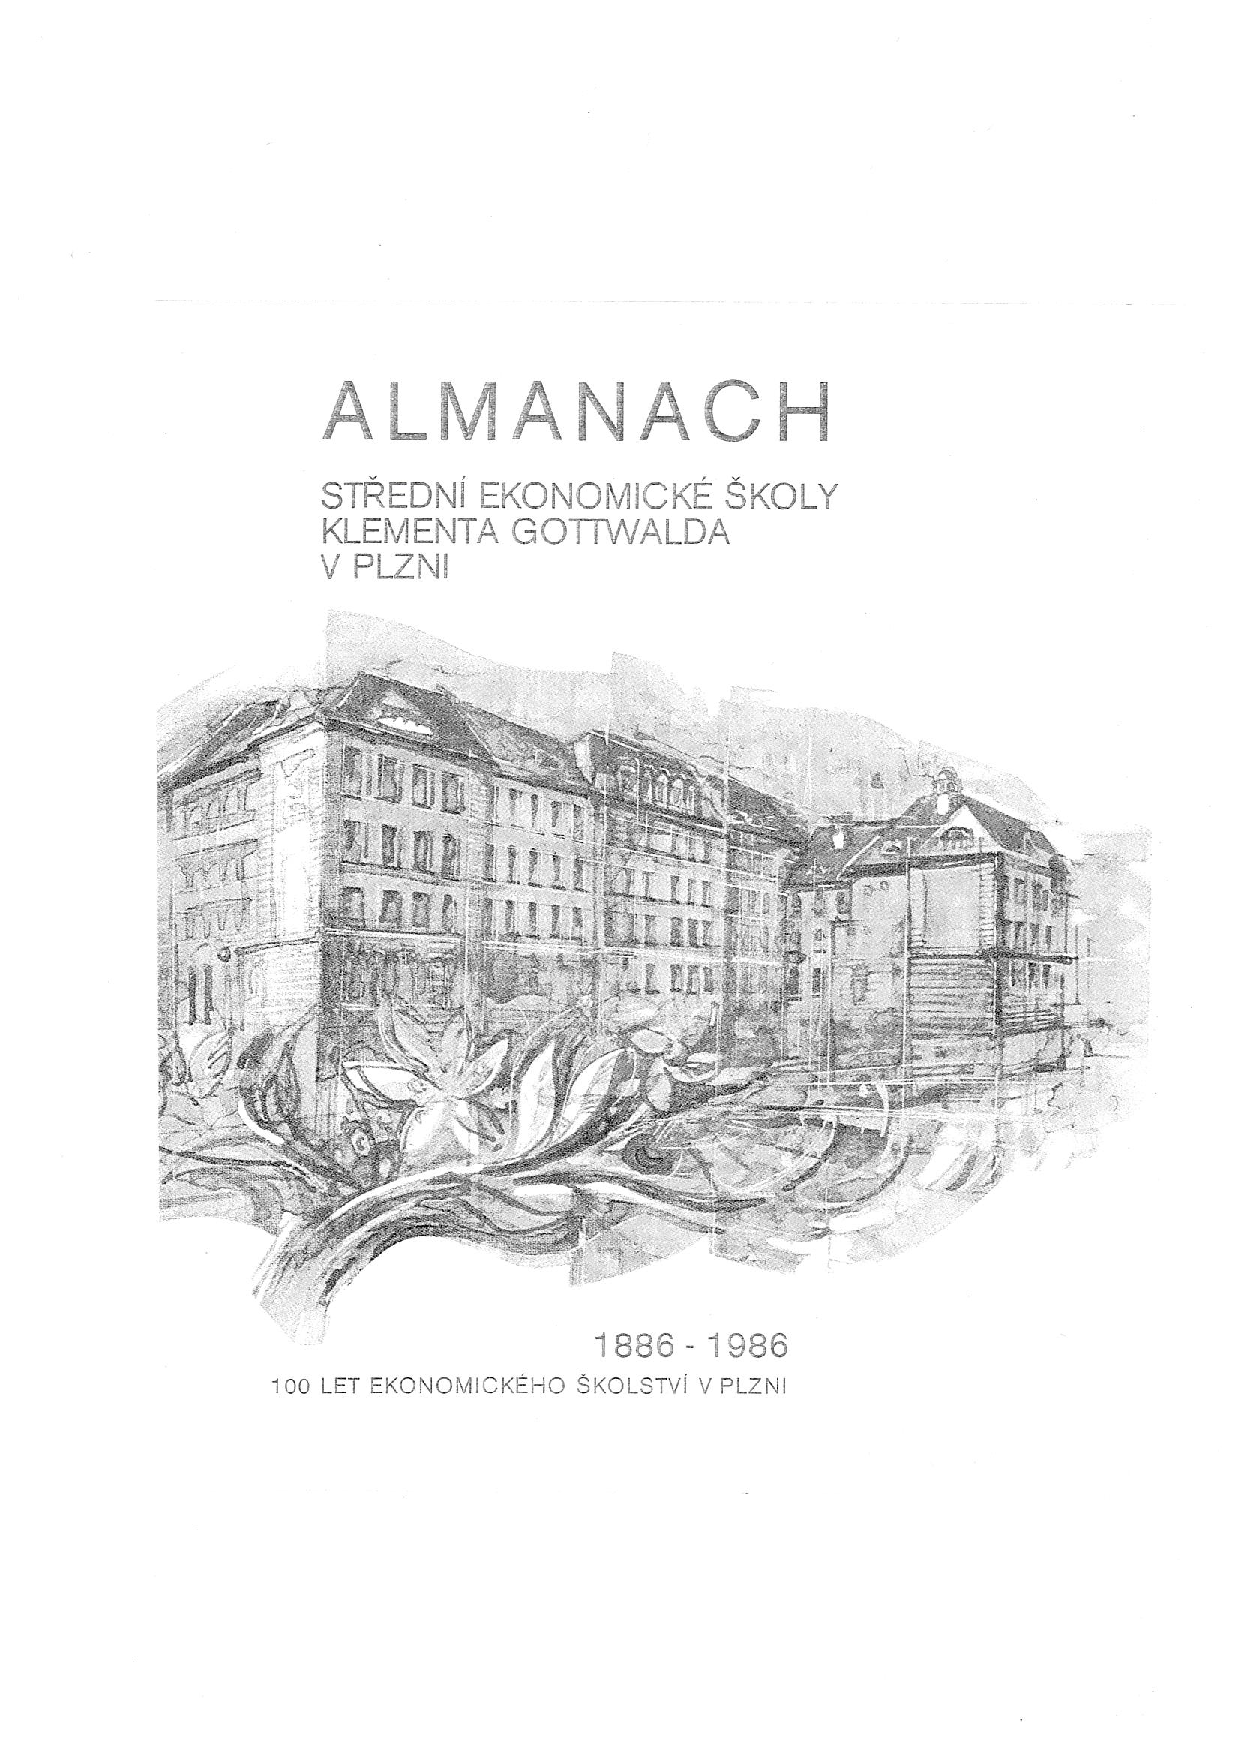
\includepdf[pages=-]{rc/almanach.pdf}

\openright
\end{document}
